\documentclass[twoside,openright,titlepage,numbers=noenddot,headinclude,%
               footinclude=true,cleardoublepage=empty,abstractoff,BCOR=5mm,%
               paper=a4,fontsize=11pt,english,dvipsnames]{scrreprt}

% Custom config ===============================================================

% Code snippets
\usepackage{minted}
\definecolor{rulecolor}{rgb}{0.80,0.80,0.80}
\definecolor{bgcolor}{rgb}{1.0,1.0,1.0}
\newminted{python}{bgcolor=bgcolor}
% Classic thesis
\usepackage{amssymb}
% ****************************************************************************************************
% classicthesis-config.tex
% formerly known as loadpackages.sty, classicthesis-ldpkg.sty, and classicthesis-preamble.sty
% Use it at the beginning of your ClassicThesis.tex, or as a LaTeX Preamble
% in your ClassicThesis.{tex,lyx} with % ****************************************************************************************************
% classicthesis-config.tex
% formerly known as loadpackages.sty, classicthesis-ldpkg.sty, and classicthesis-preamble.sty
% Use it at the beginning of your ClassicThesis.tex, or as a LaTeX Preamble
% in your ClassicThesis.{tex,lyx} with % ****************************************************************************************************
% classicthesis-config.tex
% formerly known as loadpackages.sty, classicthesis-ldpkg.sty, and classicthesis-preamble.sty
% Use it at the beginning of your ClassicThesis.tex, or as a LaTeX Preamble
% in your ClassicThesis.{tex,lyx} with \input{classicthesis-config}
% ****************************************************************************************************
% If you like the classicthesis, then I would appreciate a postcard.
% My address can be found in the file ClassicThesis.pdf. A collection
% of the postcards I received so far is available online at
% http://postcards.miede.de
% ****************************************************************************************************

% ****************************************************************************************************
% 1. Configure classicthesis for your needs here, e.g., remove "drafting" below
% in order to deactivate the time-stamp on the pages
% ****************************************************************************************************
\PassOptionsToPackage{eulerchapternumbers,listings,%drafting,%
				 pdfspacing,%floatperchapter,%linedheaders,%subfig,
				 parts,dottedtoc}{classicthesis}
% ********************************************************************
% Available options for classicthesis.sty
% (see ClassicThesis.pdf for more information):
% drafting
% parts nochapters linedheaders
% eulerchapternumbers beramono eulermath pdfspacing minionprospacing
% tocaligned dottedtoc manychapters
% listings floatperchapter subfig
% ********************************************************************

% ********************************************************************
% Triggers for this config
% ********************************************************************
\usepackage{ifthen}
\newboolean{enable-backrefs} % enable backrefs in the bibliography
\setboolean{enable-backrefs}{false} % true false
% ****************************************************************************************************


% ****************************************************************************************************
% 2. Personal data and user ad-hoc commands
% ****************************************************************************************************
\newcommand{\myTitle}{Multi-agent Reinforcement Learning\xspace}
% \newcommand{\mySubtitle}{Deep Neural Netwoks and Hybrid Approaches}
\newcommand{\myDegree}{Doktor-Ingenieur (Dr.-Ing.)\xspace}
\newcommand{\myName}{Pascal Leroy\xspace}
\newcommand{\myProf}{Put name here\xspace}
\newcommand{\myOtherProf}{Put name here\xspace}
\newcommand{\mySupervisor}{Damien Ernst\xspace}
\newcommand{\myFaculty}{Faculty of Applied Sciences\xspace}
\newcommand{\myDepartment}{Department of EE and CS\xspace}
\newcommand{\myUni}{University of Liege\xspace}
\newcommand{\myLocation}{Liege, Belgium\xspace}
\newcommand{\myTime}{July 2023\xspace}
\newcommand{\myVersion}{version 1.0\xspace}

% ********************************************************************
% Setup, finetuning, and useful commands
% ********************************************************************
\newcounter{dummy} % necessary for correct hyperlinks (to index, bib, etc.)
\newlength{\abcd} % for ab..z string length calculation
\providecommand{\mLyX}{L\kern-.1667em\lower.25em\hbox{Y}\kern-.125emX\@}
\newcommand{\ie}{i.\,e.}
\newcommand{\Ie}{I.\,e.}
\newcommand{\eg}{e.\,g.}
\newcommand{\Eg}{E.\,g.}
% ****************************************************************************************************


% ****************************************************************************************************
% 3. Loading some handy packages
% ****************************************************************************************************
% ********************************************************************
% Packages with options that might require adjustments
% ********************************************************************
\PassOptionsToPackage{latin9}{inputenc}	% latin9 (ISO-8859-9) = latin1+"Euro sign"
 \usepackage{inputenc}

\PassOptionsToPackage{american}{babel}   % change this to your language(s)
% Spanish languages need extra options in order to work with this template
%\PassOptionsToPackage{spanish,es-lcroman}{babel}
 \usepackage{babel}

\PassOptionsToPackage{square,authoryear}{natbib}
 \usepackage{natbib}

\PassOptionsToPackage{fleqn}{amsmath}		% math environments and more by the AMS
\usepackage{amsmath}
\usepackage{amstext}
\usepackage{amsfonts}
\usepackage{amssymb}

% ********************************************************************
% General useful packages
% ********************************************************************
\PassOptionsToPackage{T1}{fontenc} % T2A for cyrillics
\usepackage{fontenc}
\usepackage{lipsum}
\usepackage{textcomp} % fix warning with missing font shapes
%\usepackage{scrhack} % fix warnings when using KOMA with listings package
\usepackage{xspace} % to get the spacing after macros right
\usepackage{mparhack} % get marginpar right
\usepackage{fixltx2e} % fixes some LaTeX stuff
\PassOptionsToPackage{printonlyused,smaller}{acronym}
	\usepackage{acronym} % nice macros for handling all acronyms in the thesis
%\renewcommand*{\acsfont}[1]{\textssc{#1}} % for MinionPro
\renewcommand{\aclabelfont}[1]{{#1}\hfill} % fix the list of acronyms
% ****************************************************************************************************


% ****************************************************************************************************
% 4. Setup floats: tables, (sub)figures, and captions
% ****************************************************************************************************
\usepackage{tabularx} % better tables
\setlength{\extrarowheight}{3pt} % increase table row height
\newcommand{\tableheadline}[1]{\multicolumn{1}{c}{\spacedlowsmallcaps{#1}}}
\newcommand{\myfloatalign}{\centering} % to be used with each float for alignment
\usepackage{caption}
%\usepackage{subfig}
%\captionsetup{format=hang,font=small}
\captionsetup{format=plain, font=small, compatibility=false}
\usepackage{graphicx}
\usepackage{subcaption}
% ****************************************************************************************************


% ****************************************************************************************************
% 5. Setup code listings
% ****************************************************************************************************
\usepackage{listings}
%\lstset{emph={trueIndex,root},emphstyle=\color{BlueViolet}}%\underbar} % for special keywords
\lstset{language=[LaTeX]Tex,%C++,
    keywordstyle=\color{RoyalBlue},%\bfseries,
    basicstyle=\small\ttfamily,
    %identifierstyle=\color{NavyBlue},
    commentstyle=\color{Green}\ttfamily,
    stringstyle=\rmfamily,
    numbers=none,%left,%
    numberstyle=\scriptsize,%\tiny
    stepnumber=5,
    numbersep=8pt,
    showstringspaces=false,
    breaklines=true,
    frameround=ftff,
    frame=single,
    belowcaptionskip=.75\baselineskip
    %frame=L
}
% ****************************************************************************************************


% ****************************************************************************************************
% 6. PDFLaTeX, hyperreferences and citation backreferences
% ****************************************************************************************************
% ********************************************************************
% Using PDFLaTeX
% ********************************************************************
\PassOptionsToPackage{pdftex,hyperfootnotes=true,pdfpagelabels}{hyperref}
	\usepackage{hyperref}  % backref linktocpage pagebackref
\pdfcompresslevel=9
\pdfadjustspacing=1
\PassOptionsToPackage{pdftex}{graphicx}

% ********************************************************************
% Setup the style of the backrefs from the bibliography
% (translate the options to any language you use)
% ********************************************************************
\newcommand{\backrefnotcitedstring}{\relax}%(Not cited.)
\newcommand{\backrefcitedsinglestring}[1]{(Cited on page~#1.)}
\newcommand{\backrefcitedmultistring}[1]{(Cited on pages~#1.)}
\ifthenelse{\boolean{enable-backrefs}}%
{%
		\PassOptionsToPackage{hyperpageref}{backref}
		\usepackage{backref} % to be loaded after hyperref package
		   \renewcommand{\backreftwosep}{ and~} % separate 2 pages
		   \renewcommand{\backreflastsep}{, and~} % separate last of longer list
		   \renewcommand*{\backref}[1]{}  % disable standard
		   \renewcommand*{\backrefalt}[4]{% detailed backref
		      \ifcase #1 %
		         \backrefnotcitedstring%
		      \or%
		         \backrefcitedsinglestring{#2}%
		      \else%
		         \backrefcitedmultistring{#2}%
		      \fi}%
}{\relax}
\usepackage{ragged2e}

% ********************************************************************
% Hyperreferences
% ********************************************************************
\hypersetup{%
    %draft,	% = no hyperlinking at all (useful in b/w printouts)
    colorlinks=true, linktocpage=true, pdfstartpage=3, pdfstartview=FitV,%
    % uncomment the following line if you want to have black links (e.g., for printing)
    %colorlinks=false, linktocpage=false, pdfborder={0 0 0}, pdfstartpage=3, pdfstartview=FitV,%
    breaklinks=true, pdfpagemode=UseNone, pageanchor=true, pdfpagemode=UseOutlines,%
    plainpages=false, bookmarksnumbered, bookmarksopen=true, bookmarksopenlevel=1,%
    hypertexnames=true, pdfhighlight=/O,%nesting=true,%frenchlinks,%
    urlcolor=webbrown, linkcolor=RoyalBlue, citecolor=webgreen, %pagecolor=RoyalBlue,%
    %urlcolor=Black, linkcolor=Black, citecolor=Black, %pagecolor=Black,%
    pdftitle={\myTitle},%
    pdfauthor={\textcopyright\ \myName, \myUni, \myFaculty},%
    pdfsubject={},%
    pdfkeywords={},%
    pdfcreator={pdfLaTeX},%
    pdfproducer={LaTeX with hyperref and classicthesis}%
}

% ********************************************************************
% Setup autoreferences
% ********************************************************************
% There are some issues regarding autorefnames
% http://www.ureader.de/msg/136221647.aspx
% http://www.tex.ac.uk/cgi-bin/texfaq2html?label=latexwords
% you have to redefine the makros for the
% language you use, e.g., american, ngerman
% (as chosen when loading babel/AtBeginDocument)
% ********************************************************************
\makeatletter
\@ifpackageloaded{babel}%
    {%
       \addto\extrasamerican{%
					\renewcommand*{\figureautorefname}{Figure}%
					\renewcommand*{\tableautorefname}{Table}%
					\renewcommand*{\partautorefname}{Part}%
					\renewcommand*{\chapterautorefname}{Chapter}%
					\renewcommand*{\sectionautorefname}{Section}%
					\renewcommand*{\subsectionautorefname}{Section}%
					\renewcommand*{\subsubsectionautorefname}{Section}%
				}%
       \addto\extrasngerman{%
					\renewcommand*{\paragraphautorefname}{Absatz}%
					\renewcommand*{\subparagraphautorefname}{Unterabsatz}%
					\renewcommand*{\footnoteautorefname}{Fu\"snote}%
					\renewcommand*{\FancyVerbLineautorefname}{Zeile}%
					\renewcommand*{\theoremautorefname}{Theorem}%
					\renewcommand*{\appendixautorefname}{Anhang}%
					\renewcommand*{\equationautorefname}{Gleichung}%
					\renewcommand*{\itemautorefname}{Punkt}%
				}%
			% Fix to getting autorefs for subfigures right (thanks to Belinda Vogt for changing the definition)
			\providecommand{\subfigureautorefname}{\figureautorefname}%
    }{\relax}
\makeatother


% ****************************************************************************************************
% 7. Last calls before the bar closes
% ****************************************************************************************************
% ********************************************************************
% Development Stuff
% ********************************************************************
\listfiles
%\PassOptionsToPackage{l2tabu,orthodox,abort}{nag}
%	\usepackage{nag}
%\PassOptionsToPackage{warning, all}{onlyamsmath}
%	\usepackage{onlyamsmath}

% ********************************************************************
% Last, but not least...
% ********************************************************************
\usepackage{classicthesis}
% ****************************************************************************************************


% ****************************************************************************************************
% 8. Further adjustments (experimental)
% ****************************************************************************************************
% ********************************************************************
% Changing the text area
% ********************************************************************
%\linespread{1.05} % a bit more for Palatino
%\areaset[current]{312pt}{761pt} % 686 (factor 2.2) + 33 head + 42 head \the\footskip
%\setlength{\marginparwidth}{7em}%
%\setlength{\marginparsep}{2em}%

% ********************************************************************
% Using different fonts
% ********************************************************************
%\usepackage[oldstylenums]{kpfonts} % oldstyle notextcomp
%\usepackage[osf]{libertine}
%\usepackage{hfoldsty} % Computer Modern with osf
%\usepackage[light,condensed,math]{iwona}
%\renewcommand{\sfdefault}{iwona}
%\usepackage{lmodern} % <-- no osf support :-(
% \usepackage[T1]{fontenc}
% \usepackage{textcomp}
%\usepackage[urw-garamond]{mathdesign} <-- no osf support :-(
\usepackage{cleveref}
\newcommand{\figref}[1]{Fig.~\ref{#1}}
\usepackage{bm}
\renewcommand*{\mathbf}[1]{\ifmmode\bm{#1}\else\textbf{#1}\fi}
\usepackage{array,multirow}
\newcommand\appref{Appendix~\ref}
%\newcommand\hypref{A\ref}
\newcommand\secref{Section~\ref}



% Math new operators
\DeclareMathOperator*{\trace}{trace}
\DeclareMathOperator*{\tr}{tr}
\DeclareMathOperator*{\diag}{diag}
\DeclareMathOperator{\dt}{\, \mathrm{d}\mathit{t}}
\newcommand{\abs}[1]{\left\lvert #1 \right\rvert}

% Math braces
\newcommand{\brac}[1]{\left({#1}\right)}
\newcommand{\sbrac}[1]{\left[{#1}\right]}
\newcommand{\cbrac}[1]{\left\{{#1}\right\}}
\usepackage{mathtools}
\DeclarePairedDelimiter{\ceil}{\lceil}{\rceil}
\DeclarePairedDelimiter{\floor}{\lfloor}{\rfloor}

% TikZ
\usepackage{tikz}
\usetikzlibrary{positioning,fit,calc,decorations.pathreplacing,arrows,backgrounds,shapes}
\usetikzlibrary{automata,arrows}

% UMNN paper
\usepackage{xparse}
\usepackage[nomessages]{fp}% http://ctan.org/pkg/fp
\ExplSyntaxOn%% allow _ : as a letter
\newcommand\UMNNParam[6]{ \fp_to_decimal:n {round(#1*(#2*#4 + #3*#4^2 + #4*30*#2+31*#6 + #5*#6^2 + #6), 0)}}
\newcommand\BNAFParam[1]{ \fp_to_decimal:n {round(5*(80*#1^2 + 2*(40^2)*#1^2), 0)}}
\newcommand\mean[3]{\fp_to_decimal:n {round((#1 + #2 + #3)/3, 2)}}
\newcommand\std[3]{\fp_to_decimal:n {round(sqrt((#1^2 + #2^2 + #3^2)/3 - ((#1 + #2 + #3)/3)^2 ), 2)}}
\ExplSyntaxOff
\usepackage{arrayjobx}
\newarray\UMNNData
\readarray{UMNNData}{ \UMNNParam{5}{6}{2}{100}{4}{150} & \UMNNParam{10}{8}{2}{100}{3}{200}
                    & \UMNNParam{5}{21}{2}{512}{4}{50} & \UMNNParam{5}{43}{1}{512}{3}{50}
                    & \UMNNParam{5}{63}{2}{1024}{4}{150}}
\newarray\TrueUMNNData
\readarray{TrueUMNNData}{509465 & 814865 & 3621765 & 3455675 & 15627065}
\newarray\BNAFData
\readarray{BNAFData}{\BNAFParam{6} & \BNAFParam{8} & \BNAFParam{21} & \BNAFParam{43} & \BNAFParam{63}}
\newarray\TrueBNAFData
%\readarray{TrueBNAFData}{307264 & 544084 & 3721414 & 15566434 & 33390634}
\readarray{TrueBNAFData}{307264 & 544084 & 3721414 & 4085434 & 8757634}
\newarray\TrueNAFData
\readarray{TrueNAFData}{414213 & 401741 & 9272743 & 7487321 & 36759591}

\usepackage{siunitx}
\sisetup{output-exponent-marker = e,round-mode = figures, round-precision = 3,
  scientific-notation = true}
\newcommand\meanstd[3]{$\mean{#1}{#2}{#3}_{\pm \std{#1}{#2}{#3}}$}

\usepackage{amsthm}

\newtheorem*{assumption*}{\assumptionnumber}
\providecommand{\assumptionnumber}{}
\makeatletter
\newenvironment{assumption}[2]
 {%
  \renewcommand{\assumptionnumber}{Assumption #1-$\mathcal{#2}$}%
  \begin{assumption*}%
  \protected@edef\@currentlabel{#1-$\mathcal{#2}$}%
 }
 {%
  \end{assumption*}
 }
\makeatother

\newcommand{\hypref}[2]{\ref{#1}}

\newcommand{\bestresult}[2]{\FPeval{\m}{round(#1, 2)}\FPeval{\s}{round(#2, 2)} \StrGobbleLeft{\s}{1}[\s]${\scriptstyle \mathbf{\m_{{\pm \s}}}}$}
\newcommand{\result}[2]{\FPeval{\m}{round(#1, 2)}\FPeval{\s}{round(#2, 2)} \StrGobbleLeft{\s}{1}[\s]${\scriptstyle \m_{\scriptstyle \pm \s}}$}


%%%%%%%%%%%%%%%% New Commands %%%%%%%%%%%%%%%%%
\newcommand{\chapref}[1]{Chapter~\ref{ch:#1}}
\newcommand{\chaprefp}[1]{\lbrack Chapter~\ref{ch:#1} \rbrack}


\usepackage[many]{tcolorbox}
\definecolor{mypink1}{rgb}{0.858, 0.188, 0.478}

% Dark orange and Dark Red rgb
\definecolor{title_color}{rgb}{0.858, 0.188, 0.478}
\definecolor{chapter_outlinebordercolor}{RGB}{0, 0, 0}
\definecolor{chapter_outlinebackgroundcolor}{RGB}{0, 0, 0}
\definecolor{LightMaroon_dark}{HTML}{0C5D6B}
\colorlet{LightMaroon}{White!57!LightMaroon_dark}
\colorlet{LightBlue}{White!98!Maroon}
\colorlet{LightBluebis}{White!100!Maroon}

\newenvironment{side_note}[1]
{\centering
	\begin{tcolorbox}[float,width=.9\textwidth,title={\textit{#1}}
	    ,enhanced jigsaw, pad at break*=1mm, breakable,
	    left=3mm, right=5mm, top=1mm, bottom=1mm,
	    colback=LightBlue, boxrule=0pt, frame hidden,
	    borderline west={0.5mm}{0mm}{Maroon},
	    % borderline east={0.1mm}{0mm}{Maroon},
	    % borderline south={0.1mm}{0mm}{Maroon},
			arc=0.mm, coltitle=Maroon, colbacktitle=LightBlue]
	\small
}
{
\end{tcolorbox}

}

\newenvironment{chapter_outline}[1]
{
\begin{tcolorbox}[breakable,width=.9\textwidth
		,enhanced jigsaw, pad at break*=1mm, breakable,
    left=4mm, right=4mm, top=4mm, bottom=1mm, boxrule=0pt, frame hidden,
		% borderline south={0.5mm}{0mm}{Maroon},
		% borderline east={0.5mm}{0mm}{Maroon},
    borderline west={0.5mm}{0mm}{Maroon},
		arc=.5mm,
		title={\Large \textbf{Outline}}, coltitle=Maroon,
		colback=LightBluebis, colbacktitle=LightBluebis
		% colbacktitle=Maroon
		]
}
{
\end{tcolorbox}

}

\newcommand{\indep}{\perp}

\usepackage{diagbox}
\usepackage{geometry}% http://ctan.org/pkg/geometry
\usepackage{pdfpages}
\usepackage[chapter]{algorithm}
\usepackage{algpseudocode}


% ****************************************************************************************************

% ****************************************************************************************************
% If you like the classicthesis, then I would appreciate a postcard.
% My address can be found in the file ClassicThesis.pdf. A collection
% of the postcards I received so far is available online at
% http://postcards.miede.de
% ****************************************************************************************************

% ****************************************************************************************************
% 1. Configure classicthesis for your needs here, e.g., remove "drafting" below
% in order to deactivate the time-stamp on the pages
% ****************************************************************************************************
\PassOptionsToPackage{eulerchapternumbers,listings,%drafting,%
				 pdfspacing,%floatperchapter,%linedheaders,%subfig,
				 parts,dottedtoc}{classicthesis}
% ********************************************************************
% Available options for classicthesis.sty
% (see ClassicThesis.pdf for more information):
% drafting
% parts nochapters linedheaders
% eulerchapternumbers beramono eulermath pdfspacing minionprospacing
% tocaligned dottedtoc manychapters
% listings floatperchapter subfig
% ********************************************************************

% ********************************************************************
% Triggers for this config
% ********************************************************************
\usepackage{ifthen}
\newboolean{enable-backrefs} % enable backrefs in the bibliography
\setboolean{enable-backrefs}{false} % true false
% ****************************************************************************************************


% ****************************************************************************************************
% 2. Personal data and user ad-hoc commands
% ****************************************************************************************************
\newcommand{\myTitle}{Multi-agent Reinforcement Learning\xspace}
% \newcommand{\mySubtitle}{Deep Neural Netwoks and Hybrid Approaches}
\newcommand{\myDegree}{Doktor-Ingenieur (Dr.-Ing.)\xspace}
\newcommand{\myName}{Pascal Leroy\xspace}
\newcommand{\myProf}{Put name here\xspace}
\newcommand{\myOtherProf}{Put name here\xspace}
\newcommand{\mySupervisor}{Damien Ernst\xspace}
\newcommand{\myFaculty}{Faculty of Applied Sciences\xspace}
\newcommand{\myDepartment}{Department of EE and CS\xspace}
\newcommand{\myUni}{University of Liege\xspace}
\newcommand{\myLocation}{Liege, Belgium\xspace}
\newcommand{\myTime}{July 2023\xspace}
\newcommand{\myVersion}{version 1.0\xspace}

% ********************************************************************
% Setup, finetuning, and useful commands
% ********************************************************************
\newcounter{dummy} % necessary for correct hyperlinks (to index, bib, etc.)
\newlength{\abcd} % for ab..z string length calculation
\providecommand{\mLyX}{L\kern-.1667em\lower.25em\hbox{Y}\kern-.125emX\@}
\newcommand{\ie}{i.\,e.}
\newcommand{\Ie}{I.\,e.}
\newcommand{\eg}{e.\,g.}
\newcommand{\Eg}{E.\,g.}
% ****************************************************************************************************


% ****************************************************************************************************
% 3. Loading some handy packages
% ****************************************************************************************************
% ********************************************************************
% Packages with options that might require adjustments
% ********************************************************************
\PassOptionsToPackage{latin9}{inputenc}	% latin9 (ISO-8859-9) = latin1+"Euro sign"
 \usepackage{inputenc}

\PassOptionsToPackage{american}{babel}   % change this to your language(s)
% Spanish languages need extra options in order to work with this template
%\PassOptionsToPackage{spanish,es-lcroman}{babel}
 \usepackage{babel}

\PassOptionsToPackage{square,authoryear}{natbib}
 \usepackage{natbib}

\PassOptionsToPackage{fleqn}{amsmath}		% math environments and more by the AMS
\usepackage{amsmath}
\usepackage{amstext}
\usepackage{amsfonts}
\usepackage{amssymb}

% ********************************************************************
% General useful packages
% ********************************************************************
\PassOptionsToPackage{T1}{fontenc} % T2A for cyrillics
\usepackage{fontenc}
\usepackage{lipsum}
\usepackage{textcomp} % fix warning with missing font shapes
%\usepackage{scrhack} % fix warnings when using KOMA with listings package
\usepackage{xspace} % to get the spacing after macros right
\usepackage{mparhack} % get marginpar right
\usepackage{fixltx2e} % fixes some LaTeX stuff
\PassOptionsToPackage{printonlyused,smaller}{acronym}
	\usepackage{acronym} % nice macros for handling all acronyms in the thesis
%\renewcommand*{\acsfont}[1]{\textssc{#1}} % for MinionPro
\renewcommand{\aclabelfont}[1]{{#1}\hfill} % fix the list of acronyms
% ****************************************************************************************************


% ****************************************************************************************************
% 4. Setup floats: tables, (sub)figures, and captions
% ****************************************************************************************************
\usepackage{tabularx} % better tables
\setlength{\extrarowheight}{3pt} % increase table row height
\newcommand{\tableheadline}[1]{\multicolumn{1}{c}{\spacedlowsmallcaps{#1}}}
\newcommand{\myfloatalign}{\centering} % to be used with each float for alignment
\usepackage{caption}
%\usepackage{subfig}
%\captionsetup{format=hang,font=small}
\captionsetup{format=plain, font=small, compatibility=false}
\usepackage{graphicx}
\usepackage{subcaption}
% ****************************************************************************************************


% ****************************************************************************************************
% 5. Setup code listings
% ****************************************************************************************************
\usepackage{listings}
%\lstset{emph={trueIndex,root},emphstyle=\color{BlueViolet}}%\underbar} % for special keywords
\lstset{language=[LaTeX]Tex,%C++,
    keywordstyle=\color{RoyalBlue},%\bfseries,
    basicstyle=\small\ttfamily,
    %identifierstyle=\color{NavyBlue},
    commentstyle=\color{Green}\ttfamily,
    stringstyle=\rmfamily,
    numbers=none,%left,%
    numberstyle=\scriptsize,%\tiny
    stepnumber=5,
    numbersep=8pt,
    showstringspaces=false,
    breaklines=true,
    frameround=ftff,
    frame=single,
    belowcaptionskip=.75\baselineskip
    %frame=L
}
% ****************************************************************************************************


% ****************************************************************************************************
% 6. PDFLaTeX, hyperreferences and citation backreferences
% ****************************************************************************************************
% ********************************************************************
% Using PDFLaTeX
% ********************************************************************
\PassOptionsToPackage{pdftex,hyperfootnotes=true,pdfpagelabels}{hyperref}
	\usepackage{hyperref}  % backref linktocpage pagebackref
\pdfcompresslevel=9
\pdfadjustspacing=1
\PassOptionsToPackage{pdftex}{graphicx}

% ********************************************************************
% Setup the style of the backrefs from the bibliography
% (translate the options to any language you use)
% ********************************************************************
\newcommand{\backrefnotcitedstring}{\relax}%(Not cited.)
\newcommand{\backrefcitedsinglestring}[1]{(Cited on page~#1.)}
\newcommand{\backrefcitedmultistring}[1]{(Cited on pages~#1.)}
\ifthenelse{\boolean{enable-backrefs}}%
{%
		\PassOptionsToPackage{hyperpageref}{backref}
		\usepackage{backref} % to be loaded after hyperref package
		   \renewcommand{\backreftwosep}{ and~} % separate 2 pages
		   \renewcommand{\backreflastsep}{, and~} % separate last of longer list
		   \renewcommand*{\backref}[1]{}  % disable standard
		   \renewcommand*{\backrefalt}[4]{% detailed backref
		      \ifcase #1 %
		         \backrefnotcitedstring%
		      \or%
		         \backrefcitedsinglestring{#2}%
		      \else%
		         \backrefcitedmultistring{#2}%
		      \fi}%
}{\relax}
\usepackage{ragged2e}

% ********************************************************************
% Hyperreferences
% ********************************************************************
\hypersetup{%
    %draft,	% = no hyperlinking at all (useful in b/w printouts)
    colorlinks=true, linktocpage=true, pdfstartpage=3, pdfstartview=FitV,%
    % uncomment the following line if you want to have black links (e.g., for printing)
    %colorlinks=false, linktocpage=false, pdfborder={0 0 0}, pdfstartpage=3, pdfstartview=FitV,%
    breaklinks=true, pdfpagemode=UseNone, pageanchor=true, pdfpagemode=UseOutlines,%
    plainpages=false, bookmarksnumbered, bookmarksopen=true, bookmarksopenlevel=1,%
    hypertexnames=true, pdfhighlight=/O,%nesting=true,%frenchlinks,%
    urlcolor=webbrown, linkcolor=RoyalBlue, citecolor=webgreen, %pagecolor=RoyalBlue,%
    %urlcolor=Black, linkcolor=Black, citecolor=Black, %pagecolor=Black,%
    pdftitle={\myTitle},%
    pdfauthor={\textcopyright\ \myName, \myUni, \myFaculty},%
    pdfsubject={},%
    pdfkeywords={},%
    pdfcreator={pdfLaTeX},%
    pdfproducer={LaTeX with hyperref and classicthesis}%
}

% ********************************************************************
% Setup autoreferences
% ********************************************************************
% There are some issues regarding autorefnames
% http://www.ureader.de/msg/136221647.aspx
% http://www.tex.ac.uk/cgi-bin/texfaq2html?label=latexwords
% you have to redefine the makros for the
% language you use, e.g., american, ngerman
% (as chosen when loading babel/AtBeginDocument)
% ********************************************************************
\makeatletter
\@ifpackageloaded{babel}%
    {%
       \addto\extrasamerican{%
					\renewcommand*{\figureautorefname}{Figure}%
					\renewcommand*{\tableautorefname}{Table}%
					\renewcommand*{\partautorefname}{Part}%
					\renewcommand*{\chapterautorefname}{Chapter}%
					\renewcommand*{\sectionautorefname}{Section}%
					\renewcommand*{\subsectionautorefname}{Section}%
					\renewcommand*{\subsubsectionautorefname}{Section}%
				}%
       \addto\extrasngerman{%
					\renewcommand*{\paragraphautorefname}{Absatz}%
					\renewcommand*{\subparagraphautorefname}{Unterabsatz}%
					\renewcommand*{\footnoteautorefname}{Fu\"snote}%
					\renewcommand*{\FancyVerbLineautorefname}{Zeile}%
					\renewcommand*{\theoremautorefname}{Theorem}%
					\renewcommand*{\appendixautorefname}{Anhang}%
					\renewcommand*{\equationautorefname}{Gleichung}%
					\renewcommand*{\itemautorefname}{Punkt}%
				}%
			% Fix to getting autorefs for subfigures right (thanks to Belinda Vogt for changing the definition)
			\providecommand{\subfigureautorefname}{\figureautorefname}%
    }{\relax}
\makeatother


% ****************************************************************************************************
% 7. Last calls before the bar closes
% ****************************************************************************************************
% ********************************************************************
% Development Stuff
% ********************************************************************
\listfiles
%\PassOptionsToPackage{l2tabu,orthodox,abort}{nag}
%	\usepackage{nag}
%\PassOptionsToPackage{warning, all}{onlyamsmath}
%	\usepackage{onlyamsmath}

% ********************************************************************
% Last, but not least...
% ********************************************************************
\usepackage{classicthesis}
% ****************************************************************************************************


% ****************************************************************************************************
% 8. Further adjustments (experimental)
% ****************************************************************************************************
% ********************************************************************
% Changing the text area
% ********************************************************************
%\linespread{1.05} % a bit more for Palatino
%\areaset[current]{312pt}{761pt} % 686 (factor 2.2) + 33 head + 42 head \the\footskip
%\setlength{\marginparwidth}{7em}%
%\setlength{\marginparsep}{2em}%

% ********************************************************************
% Using different fonts
% ********************************************************************
%\usepackage[oldstylenums]{kpfonts} % oldstyle notextcomp
%\usepackage[osf]{libertine}
%\usepackage{hfoldsty} % Computer Modern with osf
%\usepackage[light,condensed,math]{iwona}
%\renewcommand{\sfdefault}{iwona}
%\usepackage{lmodern} % <-- no osf support :-(
% \usepackage[T1]{fontenc}
% \usepackage{textcomp}
%\usepackage[urw-garamond]{mathdesign} <-- no osf support :-(
\usepackage{cleveref}
\newcommand{\figref}[1]{Fig.~\ref{#1}}
\usepackage{bm}
\renewcommand*{\mathbf}[1]{\ifmmode\bm{#1}\else\textbf{#1}\fi}
\usepackage{array,multirow}
\newcommand\appref{Appendix~\ref}
%\newcommand\hypref{A\ref}
\newcommand\secref{Section~\ref}



% Math new operators
\DeclareMathOperator*{\trace}{trace}
\DeclareMathOperator*{\tr}{tr}
\DeclareMathOperator*{\diag}{diag}
\DeclareMathOperator{\dt}{\, \mathrm{d}\mathit{t}}
\newcommand{\abs}[1]{\left\lvert #1 \right\rvert}

% Math braces
\newcommand{\brac}[1]{\left({#1}\right)}
\newcommand{\sbrac}[1]{\left[{#1}\right]}
\newcommand{\cbrac}[1]{\left\{{#1}\right\}}
\usepackage{mathtools}
\DeclarePairedDelimiter{\ceil}{\lceil}{\rceil}
\DeclarePairedDelimiter{\floor}{\lfloor}{\rfloor}

% TikZ
\usepackage{tikz}
\usetikzlibrary{positioning,fit,calc,decorations.pathreplacing,arrows,backgrounds,shapes}
\usetikzlibrary{automata,arrows}

% UMNN paper
\usepackage{xparse}
\usepackage[nomessages]{fp}% http://ctan.org/pkg/fp
\ExplSyntaxOn%% allow _ : as a letter
\newcommand\UMNNParam[6]{ \fp_to_decimal:n {round(#1*(#2*#4 + #3*#4^2 + #4*30*#2+31*#6 + #5*#6^2 + #6), 0)}}
\newcommand\BNAFParam[1]{ \fp_to_decimal:n {round(5*(80*#1^2 + 2*(40^2)*#1^2), 0)}}
\newcommand\mean[3]{\fp_to_decimal:n {round((#1 + #2 + #3)/3, 2)}}
\newcommand\std[3]{\fp_to_decimal:n {round(sqrt((#1^2 + #2^2 + #3^2)/3 - ((#1 + #2 + #3)/3)^2 ), 2)}}
\ExplSyntaxOff
\usepackage{arrayjobx}
\newarray\UMNNData
\readarray{UMNNData}{ \UMNNParam{5}{6}{2}{100}{4}{150} & \UMNNParam{10}{8}{2}{100}{3}{200}
                    & \UMNNParam{5}{21}{2}{512}{4}{50} & \UMNNParam{5}{43}{1}{512}{3}{50}
                    & \UMNNParam{5}{63}{2}{1024}{4}{150}}
\newarray\TrueUMNNData
\readarray{TrueUMNNData}{509465 & 814865 & 3621765 & 3455675 & 15627065}
\newarray\BNAFData
\readarray{BNAFData}{\BNAFParam{6} & \BNAFParam{8} & \BNAFParam{21} & \BNAFParam{43} & \BNAFParam{63}}
\newarray\TrueBNAFData
%\readarray{TrueBNAFData}{307264 & 544084 & 3721414 & 15566434 & 33390634}
\readarray{TrueBNAFData}{307264 & 544084 & 3721414 & 4085434 & 8757634}
\newarray\TrueNAFData
\readarray{TrueNAFData}{414213 & 401741 & 9272743 & 7487321 & 36759591}

\usepackage{siunitx}
\sisetup{output-exponent-marker = e,round-mode = figures, round-precision = 3,
  scientific-notation = true}
\newcommand\meanstd[3]{$\mean{#1}{#2}{#3}_{\pm \std{#1}{#2}{#3}}$}

\usepackage{amsthm}

\newtheorem*{assumption*}{\assumptionnumber}
\providecommand{\assumptionnumber}{}
\makeatletter
\newenvironment{assumption}[2]
 {%
  \renewcommand{\assumptionnumber}{Assumption #1-$\mathcal{#2}$}%
  \begin{assumption*}%
  \protected@edef\@currentlabel{#1-$\mathcal{#2}$}%
 }
 {%
  \end{assumption*}
 }
\makeatother

\newcommand{\hypref}[2]{\ref{#1}}

\newcommand{\bestresult}[2]{\FPeval{\m}{round(#1, 2)}\FPeval{\s}{round(#2, 2)} \StrGobbleLeft{\s}{1}[\s]${\scriptstyle \mathbf{\m_{{\pm \s}}}}$}
\newcommand{\result}[2]{\FPeval{\m}{round(#1, 2)}\FPeval{\s}{round(#2, 2)} \StrGobbleLeft{\s}{1}[\s]${\scriptstyle \m_{\scriptstyle \pm \s}}$}


%%%%%%%%%%%%%%%% New Commands %%%%%%%%%%%%%%%%%
\newcommand{\chapref}[1]{Chapter~\ref{ch:#1}}
\newcommand{\chaprefp}[1]{\lbrack Chapter~\ref{ch:#1} \rbrack}


\usepackage[many]{tcolorbox}
\definecolor{mypink1}{rgb}{0.858, 0.188, 0.478}

% Dark orange and Dark Red rgb
\definecolor{title_color}{rgb}{0.858, 0.188, 0.478}
\definecolor{chapter_outlinebordercolor}{RGB}{0, 0, 0}
\definecolor{chapter_outlinebackgroundcolor}{RGB}{0, 0, 0}
\definecolor{LightMaroon_dark}{HTML}{0C5D6B}
\colorlet{LightMaroon}{White!57!LightMaroon_dark}
\colorlet{LightBlue}{White!98!Maroon}
\colorlet{LightBluebis}{White!100!Maroon}

\newenvironment{side_note}[1]
{\centering
	\begin{tcolorbox}[float,width=.9\textwidth,title={\textit{#1}}
	    ,enhanced jigsaw, pad at break*=1mm, breakable,
	    left=3mm, right=5mm, top=1mm, bottom=1mm,
	    colback=LightBlue, boxrule=0pt, frame hidden,
	    borderline west={0.5mm}{0mm}{Maroon},
	    % borderline east={0.1mm}{0mm}{Maroon},
	    % borderline south={0.1mm}{0mm}{Maroon},
			arc=0.mm, coltitle=Maroon, colbacktitle=LightBlue]
	\small
}
{
\end{tcolorbox}

}

\newenvironment{chapter_outline}[1]
{
\begin{tcolorbox}[breakable,width=.9\textwidth
		,enhanced jigsaw, pad at break*=1mm, breakable,
    left=4mm, right=4mm, top=4mm, bottom=1mm, boxrule=0pt, frame hidden,
		% borderline south={0.5mm}{0mm}{Maroon},
		% borderline east={0.5mm}{0mm}{Maroon},
    borderline west={0.5mm}{0mm}{Maroon},
		arc=.5mm,
		title={\Large \textbf{Outline}}, coltitle=Maroon,
		colback=LightBluebis, colbacktitle=LightBluebis
		% colbacktitle=Maroon
		]
}
{
\end{tcolorbox}

}

\newcommand{\indep}{\perp}

\usepackage{diagbox}
\usepackage{geometry}% http://ctan.org/pkg/geometry
\usepackage{pdfpages}
\usepackage[chapter]{algorithm}
\usepackage{algpseudocode}


% ****************************************************************************************************

% ****************************************************************************************************
% If you like the classicthesis, then I would appreciate a postcard.
% My address can be found in the file ClassicThesis.pdf. A collection
% of the postcards I received so far is available online at
% http://postcards.miede.de
% ****************************************************************************************************

% ****************************************************************************************************
% 1. Configure classicthesis for your needs here, e.g., remove "drafting" below
% in order to deactivate the time-stamp on the pages
% ****************************************************************************************************
\PassOptionsToPackage{eulerchapternumbers,listings,%drafting,%
				 pdfspacing,%floatperchapter,%linedheaders,%subfig,
				 parts,dottedtoc}{classicthesis}
% ********************************************************************
% Available options for classicthesis.sty
% (see ClassicThesis.pdf for more information):
% drafting
% parts nochapters linedheaders
% eulerchapternumbers beramono eulermath pdfspacing minionprospacing
% tocaligned dottedtoc manychapters
% listings floatperchapter subfig
% ********************************************************************

% ********************************************************************
% Triggers for this config
% ********************************************************************
\usepackage{ifthen}
\newboolean{enable-backrefs} % enable backrefs in the bibliography
\setboolean{enable-backrefs}{false} % true false
% ****************************************************************************************************


% ****************************************************************************************************
% 2. Personal data and user ad-hoc commands
% ****************************************************************************************************
\newcommand{\myTitle}{Multi-agent Reinforcement Learning\xspace}
% \newcommand{\mySubtitle}{Deep Neural Netwoks and Hybrid Approaches}
\newcommand{\myDegree}{Doktor-Ingenieur (Dr.-Ing.)\xspace}
\newcommand{\myName}{Pascal Leroy\xspace}
\newcommand{\myProf}{Put name here\xspace}
\newcommand{\myOtherProf}{Put name here\xspace}
\newcommand{\mySupervisor}{Damien Ernst\xspace}
\newcommand{\myFaculty}{Faculty of Applied Sciences\xspace}
\newcommand{\myDepartment}{Department of EE and CS\xspace}
\newcommand{\myUni}{University of Liege\xspace}
\newcommand{\myLocation}{Liege, Belgium\xspace}
\newcommand{\myTime}{July 2023\xspace}
\newcommand{\myVersion}{version 1.0\xspace}

% ********************************************************************
% Setup, finetuning, and useful commands
% ********************************************************************
\newcounter{dummy} % necessary for correct hyperlinks (to index, bib, etc.)
\newlength{\abcd} % for ab..z string length calculation
\providecommand{\mLyX}{L\kern-.1667em\lower.25em\hbox{Y}\kern-.125emX\@}
\newcommand{\ie}{i.\,e.}
\newcommand{\Ie}{I.\,e.}
\newcommand{\eg}{e.\,g.}
\newcommand{\Eg}{E.\,g.}
% ****************************************************************************************************


% ****************************************************************************************************
% 3. Loading some handy packages
% ****************************************************************************************************
% ********************************************************************
% Packages with options that might require adjustments
% ********************************************************************
\PassOptionsToPackage{latin9}{inputenc}	% latin9 (ISO-8859-9) = latin1+"Euro sign"
 \usepackage{inputenc}

\PassOptionsToPackage{american}{babel}   % change this to your language(s)
% Spanish languages need extra options in order to work with this template
%\PassOptionsToPackage{spanish,es-lcroman}{babel}
 \usepackage{babel}

\PassOptionsToPackage{square,authoryear}{natbib}
 \usepackage{natbib}

\PassOptionsToPackage{fleqn}{amsmath}		% math environments and more by the AMS
\usepackage{amsmath}
\usepackage{amstext}
\usepackage{amsfonts}
\usepackage{amssymb}

% ********************************************************************
% General useful packages
% ********************************************************************
\PassOptionsToPackage{T1}{fontenc} % T2A for cyrillics
\usepackage{fontenc}
\usepackage{lipsum}
\usepackage{textcomp} % fix warning with missing font shapes
%\usepackage{scrhack} % fix warnings when using KOMA with listings package
\usepackage{xspace} % to get the spacing after macros right
\usepackage{mparhack} % get marginpar right
\usepackage{fixltx2e} % fixes some LaTeX stuff
\PassOptionsToPackage{printonlyused,smaller}{acronym}
	\usepackage{acronym} % nice macros for handling all acronyms in the thesis
%\renewcommand*{\acsfont}[1]{\textssc{#1}} % for MinionPro
\renewcommand{\aclabelfont}[1]{{#1}\hfill} % fix the list of acronyms
% ****************************************************************************************************


% ****************************************************************************************************
% 4. Setup floats: tables, (sub)figures, and captions
% ****************************************************************************************************
\usepackage{tabularx} % better tables
\setlength{\extrarowheight}{3pt} % increase table row height
\newcommand{\tableheadline}[1]{\multicolumn{1}{c}{\spacedlowsmallcaps{#1}}}
\newcommand{\myfloatalign}{\centering} % to be used with each float for alignment
\usepackage{caption}
%\usepackage{subfig}
%\captionsetup{format=hang,font=small}
\captionsetup{format=plain, font=small, compatibility=false}
\usepackage{graphicx}
\usepackage{subcaption}
% ****************************************************************************************************


% ****************************************************************************************************
% 5. Setup code listings
% ****************************************************************************************************
\usepackage{listings}
%\lstset{emph={trueIndex,root},emphstyle=\color{BlueViolet}}%\underbar} % for special keywords
\lstset{language=[LaTeX]Tex,%C++,
    keywordstyle=\color{RoyalBlue},%\bfseries,
    basicstyle=\small\ttfamily,
    %identifierstyle=\color{NavyBlue},
    commentstyle=\color{Green}\ttfamily,
    stringstyle=\rmfamily,
    numbers=none,%left,%
    numberstyle=\scriptsize,%\tiny
    stepnumber=5,
    numbersep=8pt,
    showstringspaces=false,
    breaklines=true,
    frameround=ftff,
    frame=single,
    belowcaptionskip=.75\baselineskip
    %frame=L
}
% ****************************************************************************************************


% ****************************************************************************************************
% 6. PDFLaTeX, hyperreferences and citation backreferences
% ****************************************************************************************************
% ********************************************************************
% Using PDFLaTeX
% ********************************************************************
\PassOptionsToPackage{pdftex,hyperfootnotes=true,pdfpagelabels}{hyperref}
	\usepackage{hyperref}  % backref linktocpage pagebackref
\pdfcompresslevel=9
\pdfadjustspacing=1
\PassOptionsToPackage{pdftex}{graphicx}

% ********************************************************************
% Setup the style of the backrefs from the bibliography
% (translate the options to any language you use)
% ********************************************************************
\newcommand{\backrefnotcitedstring}{\relax}%(Not cited.)
\newcommand{\backrefcitedsinglestring}[1]{(Cited on page~#1.)}
\newcommand{\backrefcitedmultistring}[1]{(Cited on pages~#1.)}
\ifthenelse{\boolean{enable-backrefs}}%
{%
		\PassOptionsToPackage{hyperpageref}{backref}
		\usepackage{backref} % to be loaded after hyperref package
		   \renewcommand{\backreftwosep}{ and~} % separate 2 pages
		   \renewcommand{\backreflastsep}{, and~} % separate last of longer list
		   \renewcommand*{\backref}[1]{}  % disable standard
		   \renewcommand*{\backrefalt}[4]{% detailed backref
		      \ifcase #1 %
		         \backrefnotcitedstring%
		      \or%
		         \backrefcitedsinglestring{#2}%
		      \else%
		         \backrefcitedmultistring{#2}%
		      \fi}%
}{\relax}
\usepackage{ragged2e}

% ********************************************************************
% Hyperreferences
% ********************************************************************
\hypersetup{%
    %draft,	% = no hyperlinking at all (useful in b/w printouts)
    colorlinks=true, linktocpage=true, pdfstartpage=3, pdfstartview=FitV,%
    % uncomment the following line if you want to have black links (e.g., for printing)
    %colorlinks=false, linktocpage=false, pdfborder={0 0 0}, pdfstartpage=3, pdfstartview=FitV,%
    breaklinks=true, pdfpagemode=UseNone, pageanchor=true, pdfpagemode=UseOutlines,%
    plainpages=false, bookmarksnumbered, bookmarksopen=true, bookmarksopenlevel=1,%
    hypertexnames=true, pdfhighlight=/O,%nesting=true,%frenchlinks,%
    urlcolor=webbrown, linkcolor=RoyalBlue, citecolor=webgreen, %pagecolor=RoyalBlue,%
    %urlcolor=Black, linkcolor=Black, citecolor=Black, %pagecolor=Black,%
    pdftitle={\myTitle},%
    pdfauthor={\textcopyright\ \myName, \myUni, \myFaculty},%
    pdfsubject={},%
    pdfkeywords={},%
    pdfcreator={pdfLaTeX},%
    pdfproducer={LaTeX with hyperref and classicthesis}%
}

% ********************************************************************
% Setup autoreferences
% ********************************************************************
% There are some issues regarding autorefnames
% http://www.ureader.de/msg/136221647.aspx
% http://www.tex.ac.uk/cgi-bin/texfaq2html?label=latexwords
% you have to redefine the makros for the
% language you use, e.g., american, ngerman
% (as chosen when loading babel/AtBeginDocument)
% ********************************************************************
\makeatletter
\@ifpackageloaded{babel}%
    {%
       \addto\extrasamerican{%
					\renewcommand*{\figureautorefname}{Figure}%
					\renewcommand*{\tableautorefname}{Table}%
					\renewcommand*{\partautorefname}{Part}%
					\renewcommand*{\chapterautorefname}{Chapter}%
					\renewcommand*{\sectionautorefname}{Section}%
					\renewcommand*{\subsectionautorefname}{Section}%
					\renewcommand*{\subsubsectionautorefname}{Section}%
				}%
       \addto\extrasngerman{%
					\renewcommand*{\paragraphautorefname}{Absatz}%
					\renewcommand*{\subparagraphautorefname}{Unterabsatz}%
					\renewcommand*{\footnoteautorefname}{Fu\"snote}%
					\renewcommand*{\FancyVerbLineautorefname}{Zeile}%
					\renewcommand*{\theoremautorefname}{Theorem}%
					\renewcommand*{\appendixautorefname}{Anhang}%
					\renewcommand*{\equationautorefname}{Gleichung}%
					\renewcommand*{\itemautorefname}{Punkt}%
				}%
			% Fix to getting autorefs for subfigures right (thanks to Belinda Vogt for changing the definition)
			\providecommand{\subfigureautorefname}{\figureautorefname}%
    }{\relax}
\makeatother


% ****************************************************************************************************
% 7. Last calls before the bar closes
% ****************************************************************************************************
% ********************************************************************
% Development Stuff
% ********************************************************************
\listfiles
%\PassOptionsToPackage{l2tabu,orthodox,abort}{nag}
%	\usepackage{nag}
%\PassOptionsToPackage{warning, all}{onlyamsmath}
%	\usepackage{onlyamsmath}

% ********************************************************************
% Last, but not least...
% ********************************************************************
\usepackage{classicthesis}
% ****************************************************************************************************


% ****************************************************************************************************
% 8. Further adjustments (experimental)
% ****************************************************************************************************
% ********************************************************************
% Changing the text area
% ********************************************************************
%\linespread{1.05} % a bit more for Palatino
%\areaset[current]{312pt}{761pt} % 686 (factor 2.2) + 33 head + 42 head \the\footskip
%\setlength{\marginparwidth}{7em}%
%\setlength{\marginparsep}{2em}%

% ********************************************************************
% Using different fonts
% ********************************************************************
%\usepackage[oldstylenums]{kpfonts} % oldstyle notextcomp
%\usepackage[osf]{libertine}
%\usepackage{hfoldsty} % Computer Modern with osf
%\usepackage[light,condensed,math]{iwona}
%\renewcommand{\sfdefault}{iwona}
%\usepackage{lmodern} % <-- no osf support :-(
% \usepackage[T1]{fontenc}
% \usepackage{textcomp}
%\usepackage[urw-garamond]{mathdesign} <-- no osf support :-(
\usepackage{cleveref}
\newcommand{\figref}[1]{Fig.~\ref{#1}}
\usepackage{bm}
\renewcommand*{\mathbf}[1]{\ifmmode\bm{#1}\else\textbf{#1}\fi}
\usepackage{array,multirow}
\newcommand\appref{Appendix~\ref}
%\newcommand\hypref{A\ref}
\newcommand\secref{Section~\ref}



% Math new operators
\DeclareMathOperator*{\trace}{trace}
\DeclareMathOperator*{\tr}{tr}
\DeclareMathOperator*{\diag}{diag}
\DeclareMathOperator{\dt}{\, \mathrm{d}\mathit{t}}
\newcommand{\abs}[1]{\left\lvert #1 \right\rvert}

% Math braces
\newcommand{\brac}[1]{\left({#1}\right)}
\newcommand{\sbrac}[1]{\left[{#1}\right]}
\newcommand{\cbrac}[1]{\left\{{#1}\right\}}
\usepackage{mathtools}
\DeclarePairedDelimiter{\ceil}{\lceil}{\rceil}
\DeclarePairedDelimiter{\floor}{\lfloor}{\rfloor}

% TikZ
\usepackage{tikz}
\usetikzlibrary{positioning,fit,calc,decorations.pathreplacing,arrows,backgrounds,shapes}
\usetikzlibrary{automata,arrows}

% UMNN paper
\usepackage{xparse}
\usepackage[nomessages]{fp}% http://ctan.org/pkg/fp
\ExplSyntaxOn%% allow _ : as a letter
\newcommand\UMNNParam[6]{ \fp_to_decimal:n {round(#1*(#2*#4 + #3*#4^2 + #4*30*#2+31*#6 + #5*#6^2 + #6), 0)}}
\newcommand\BNAFParam[1]{ \fp_to_decimal:n {round(5*(80*#1^2 + 2*(40^2)*#1^2), 0)}}
\newcommand\mean[3]{\fp_to_decimal:n {round((#1 + #2 + #3)/3, 2)}}
\newcommand\std[3]{\fp_to_decimal:n {round(sqrt((#1^2 + #2^2 + #3^2)/3 - ((#1 + #2 + #3)/3)^2 ), 2)}}
\ExplSyntaxOff
\usepackage{arrayjobx}
\newarray\UMNNData
\readarray{UMNNData}{ \UMNNParam{5}{6}{2}{100}{4}{150} & \UMNNParam{10}{8}{2}{100}{3}{200}
                    & \UMNNParam{5}{21}{2}{512}{4}{50} & \UMNNParam{5}{43}{1}{512}{3}{50}
                    & \UMNNParam{5}{63}{2}{1024}{4}{150}}
\newarray\TrueUMNNData
\readarray{TrueUMNNData}{509465 & 814865 & 3621765 & 3455675 & 15627065}
\newarray\BNAFData
\readarray{BNAFData}{\BNAFParam{6} & \BNAFParam{8} & \BNAFParam{21} & \BNAFParam{43} & \BNAFParam{63}}
\newarray\TrueBNAFData
%\readarray{TrueBNAFData}{307264 & 544084 & 3721414 & 15566434 & 33390634}
\readarray{TrueBNAFData}{307264 & 544084 & 3721414 & 4085434 & 8757634}
\newarray\TrueNAFData
\readarray{TrueNAFData}{414213 & 401741 & 9272743 & 7487321 & 36759591}

\usepackage{siunitx}
\sisetup{output-exponent-marker = e,round-mode = figures, round-precision = 3,
  scientific-notation = true}
\newcommand\meanstd[3]{$\mean{#1}{#2}{#3}_{\pm \std{#1}{#2}{#3}}$}

\usepackage{amsthm}

\newtheorem*{assumption*}{\assumptionnumber}
\providecommand{\assumptionnumber}{}
\makeatletter
\newenvironment{assumption}[2]
 {%
  \renewcommand{\assumptionnumber}{Assumption #1-$\mathcal{#2}$}%
  \begin{assumption*}%
  \protected@edef\@currentlabel{#1-$\mathcal{#2}$}%
 }
 {%
  \end{assumption*}
 }
\makeatother

\newcommand{\hypref}[2]{\ref{#1}}

\newcommand{\bestresult}[2]{\FPeval{\m}{round(#1, 2)}\FPeval{\s}{round(#2, 2)} \StrGobbleLeft{\s}{1}[\s]${\scriptstyle \mathbf{\m_{{\pm \s}}}}$}
\newcommand{\result}[2]{\FPeval{\m}{round(#1, 2)}\FPeval{\s}{round(#2, 2)} \StrGobbleLeft{\s}{1}[\s]${\scriptstyle \m_{\scriptstyle \pm \s}}$}


%%%%%%%%%%%%%%%% New Commands %%%%%%%%%%%%%%%%%
\newcommand{\chapref}[1]{Chapter~\ref{ch:#1}}
\newcommand{\chaprefp}[1]{\lbrack Chapter~\ref{ch:#1} \rbrack}


\usepackage[many]{tcolorbox}
\definecolor{mypink1}{rgb}{0.858, 0.188, 0.478}

% Dark orange and Dark Red rgb
\definecolor{title_color}{rgb}{0.858, 0.188, 0.478}
\definecolor{chapter_outlinebordercolor}{RGB}{0, 0, 0}
\definecolor{chapter_outlinebackgroundcolor}{RGB}{0, 0, 0}
\definecolor{LightMaroon_dark}{HTML}{0C5D6B}
\colorlet{LightMaroon}{White!57!LightMaroon_dark}
\colorlet{LightBlue}{White!98!Maroon}
\colorlet{LightBluebis}{White!100!Maroon}

\newenvironment{side_note}[1]
{\centering
	\begin{tcolorbox}[float,width=.9\textwidth,title={\textit{#1}}
	    ,enhanced jigsaw, pad at break*=1mm, breakable,
	    left=3mm, right=5mm, top=1mm, bottom=1mm,
	    colback=LightBlue, boxrule=0pt, frame hidden,
	    borderline west={0.5mm}{0mm}{Maroon},
	    % borderline east={0.1mm}{0mm}{Maroon},
	    % borderline south={0.1mm}{0mm}{Maroon},
			arc=0.mm, coltitle=Maroon, colbacktitle=LightBlue]
	\small
}
{
\end{tcolorbox}

}

\newenvironment{chapter_outline}[1]
{
\begin{tcolorbox}[breakable,width=.9\textwidth
		,enhanced jigsaw, pad at break*=1mm, breakable,
    left=4mm, right=4mm, top=4mm, bottom=1mm, boxrule=0pt, frame hidden,
		% borderline south={0.5mm}{0mm}{Maroon},
		% borderline east={0.5mm}{0mm}{Maroon},
    borderline west={0.5mm}{0mm}{Maroon},
		arc=.5mm,
		title={\Large \textbf{Outline}}, coltitle=Maroon,
		colback=LightBluebis, colbacktitle=LightBluebis
		% colbacktitle=Maroon
		]
}
{
\end{tcolorbox}

}

\newcommand{\indep}{\perp}

\usepackage{diagbox}
\usepackage{geometry}% http://ctan.org/pkg/geometry
\usepackage{pdfpages}
\usepackage[chapter]{algorithm}
\usepackage{algpseudocode}


% ****************************************************************************************************



% Theorems and definitions
\usepackage{amsthm}
\newtheorem{theorem}{Theorem}
\newtheorem{lemma}[theorem]{Lemma}
\newtheorem{proposition}[theorem]{Proposition}
\newtheorem{corollary}[theorem]{Corollary}
\newtheorem{definition}{Definition}

% \newtheorem{algorithm}{Algorithm}
% \usepackage{algpseudocode}

% Counters
\renewcommand{\labelenumi}{{\color{halfgray}(\alph{enumi})}}
\renewcommand{\labelenumii}{\color{halfgray}{\roman{enumii}.}}
\renewcommand{\labelitemi}{{\color{halfgray}-}}%\raisebox{0.3ex}{\tiny$\blacksquare$}}}

\numberwithin{theorem}{chapter}
\numberwithin{definition}{chapter}
\numberwithin{algorithm}{chapter}
\numberwithin{figure}{chapter}
\numberwithin{table}{chapter}


\usepackage{tikz}

% Maths
\DeclareMathOperator*{\argmin}{arg\,min}
\DeclareMathOperator*{\argmax}{arg\,max}

\numberwithin{equation}{chapter}
\allowdisplaybreaks

% Shaded boxes
\usepackage{framed}
\newenvironment{remark}[1]{%
  \definecolor{shadecolor}{gray}{0.9}%
  \begin{shaded}{\color{Maroon}\noindent\textsc{#1}}\\%
}{%
  \end{shaded}%
}


% Todo
\newcommand{\todo}[1]{\textcolor{red}{[TODO] #1}}
\newcommand{\damien}[1]{\textbf{\textcolor{red}{[Damien] #1}}}

% PS pictures
\usepackage{pstricks,auto-pst-pdf}

% Landscape tables
\usepackage{rotating}


% Checkmarks
\usepackage{pifont}% http://ctan.org/pkg/pifont
\newcommand{\cmark}{\ding{51}}%
\newcommand{\xmark}{\ding{55}}%

% Wide tables
\usepackage{ltablex}
\usepackage{colortbl} % colorcell
\usepackage[dvipsnames]{xcolor}

\usepackage{multirow}
\usepackage{color}

% -----------------------------------------------------------------------------

\begin{document}

\usetikzlibrary{positioning, shapes.geometric, arrows.meta, calc}


\frenchspacing
\raggedbottom
\selectlanguage{american}
\pagenumbering{roman}
\pagestyle{plain}


% Front pages =================================================================
% Front page ==================================================================
\newgeometry{margin=0in}
\begin{titlepage}
	\begin{tikzpicture}[remember picture, overlay]
	  \node[opacity=0.6,inner sep=0pt] at (current page.center)
	   {};
	\end{tikzpicture}
    \begin{center}
    \large
	\vspace{2em}
	% \rule{20cm}{0.4pt}\\
		\begin{addmargin}[3cm]{3cm}
		\begin{center}

	        {\Large \textsc{University of Li{\`e}ge}}\\[1ex]
	        School of Engineering\\[1ex]
	        Department of Electrical Engineering \& Computer Science\\
		\end{center}

		\end{addmargin}

	% \rule{20cm}{0.4pt}\\

		\begin{addmargin}[3cm]{3cm}
		\begin{center}

			\vspace{3.5cm}
			\vspace{3cm}
	        \rule{14cm}{0.4pt}\\ \bigskip
	        \begingroup
	            \Large
	            \spacedallcaps{Multi-agent Reinforcement Learning} \\ 
				\bigskip
	        \endgroup
	        \rule{14cm}{0.4pt}\\
			\vspace{3cm}
			a PhD dissertation\\[1ex]
			by \textsc{Pascal Leroy}
		\end{center}
		\end{addmargin}
    \end{center}

	\vspace{5.5cm}

	\begin{minipage}[t]{.3\textwidth}
		
\includegraphics[width=1.\textwidth]{figures/blason.pdf}
	\end{minipage}
	\begin{minipage}[t]{.6\textwidth}
		\raggedleft
		\vspace{-2.5cm}
		\hfill Advisors: \\
		\hfill Prof. \textsc{Damien Ernst}\\
		\hfill Dr \textsc{Jonathan Pisane} \\
		\hfill July 2023
	\end{minipage}
\end{titlepage}
\restoregeometry

\cleardoublepage% Disclaimer ====================================================================

\vspace*{\fill}
\vspace*{\fill}
\vspace*{\fill}
\begin{center}
\textit{
This dissertation has been submitted in partial fulfilment of
the requirements for the Degree of Doctor of Philosophy in
Computer Science.
}
\end{center}

\vspace*{\fill}
\vspace*{\fill}
\vspace*{\fill}

%\cleardoublepage% Jury ====================================================================

\pdfbookmark[1]{Jury members}{Jury members}
\chapter*{Jury members}


\noindent \textsc{TBD}, Professor at ;\\

\noindent \textsc{TBD}, Professor at . \\

\cleardoublepage% Abstract ====================================================================

\pdfbookmark[1]{Abstract}{Abstract}
\chapter*{Abstract}

In the realm of machine learning, multi-agent reinforcement learning (MARL) is the setting where several agents learn to act by receiving rewards after deciding on actions based on their perception of their environment.
It takes its foundation in game theory and reinforcement learning (RL), both fields developed for decades.
The success of deep neural networks is leading to unprecedented progress in the variety of problems that can be solved by such methods.
Indeed, many real-world applications, such as autonomous vehicles, swarms of drones, warehouse houses, cyber securities, traffic management, or smart grids, can be framed as MARL ones.
In this thesis, we present contributions in this domain, particularly in training a team of agents to cooperate alone or against opposing teams.
This manuscript starts with the fundamentals, defining the general MARL framework and how it is divided into the settings of cooperation, competition, and general sum.
It also provides the necessary background for the unfamiliar reader with RL.

The second part of the thesis is dedicated to the cooperative setting, where agents share the same goal.
Such a setting is commonly framed as a decentralised, partially observable Markov decision process (Dec-POMDP).
This second part begins with a background chapter defining the Dec-POMDP and how it is solved in the literature.
The following chapters present two contributions to the cooperative MARL field at the foundation of this thesis.
One concerns methods extending the Deep-Quality-Value family of algorithms to the cooperative, demonstrating competitive performance with the state of the art of their time.
The other presents IMP-MARL, an open-source suite of MARL environments for large-scale infrastructure management planning (IMP).
In IMP, inspections, repairs and/or retrofits should be decided to control the risk of potential system failures, such as bridge or wind turbine failures.

The third part of the thesis addresses the problem of training a team against an opposing one.
This setting extends the competition setting, framed as agents having opposing goals, to teams of agents having opposing goals.
It is composed of two chapters.
The former present historical stories and solutions from game theory to the competition and general sum setting.
The latter presents the third contribution which is a study on how to pair cooperative and competitive methods to train a team in a two-team Markov game with the objective to be resilient to many strategies.

Finally, the manuscript concludes with a retrospective of the scientific findings provided by the contributions at the foundation of this thesis and a discussion on the societal impact that MARL has the potential to provide in the upcoming years.


%\cleardoublepage\include{frontback/publications}
%\cleardoublepage% Acknowledgements ============================================================

\pdfbookmark[1]{Acknowledgments}{acknowledgments}
\chapter*{Acknowledgments}
This is the first sentence of the acknowledgments
\pagestyle{scrheadings}
\cleardoublepage% Table of contents ===========================================================

\refstepcounter{dummy}
\pdfbookmark[1]{\contentsname}{tableofcontents}
\setcounter{tocdepth}{3} % <-- 2 includes up to subsections in the ToC
\setcounter{secnumdepth}{3} % <-- 3 numbers up to subsubsections
\manualmark
\markboth{\spacedlowsmallcaps{\contentsname}}{\spacedlowsmallcaps{\contentsname}}
\tableofcontents
\automark[section]{chapter}
\renewcommand{\chaptermark}[1]{\markboth{\spacedlowsmallcaps{#1}}{\spacedlowsmallcaps{#1}}}
\renewcommand{\sectionmark}[1]{\markright{\thesection\enspace\spacedlowsmallcaps{#1}}}

\cleardoublepage



% Content =====================================================================
\pagenumbering{arabic}

\cleardoublepage

\chapter{Introduction}\label{ch:introduction}
\damien{Deadline: 13/02}

We all make decisions.
A decision is a choice among possibilities, and different kinds of decisions exist.
For example, consider yourself driving a car and arriving at a crossroads.
In front of you, there is a traffic sign.
Based on your perception and knowledge, you first decide it is a stop sign.
This decision involves reasoning, even if it may be almost instantaneous.
But this decision has no impact on the car.
Secondly, when you decide to stop the car, as suggested by the sign, you decide to take the action of stopping it.
This second decision, based on the first one, impacts your environment.
Indeed, you push on the brakes, and the car decelerates until it stops.
This highlights one of the differences between decisions, which we differentiate as acting or reasoning.
Their impact can often distinguish them: acting usually affects our environment while reasoning doesn't.

Decisions are based on what we have learned.
You studied the traffic signs to know it was a stop one.
You practised your driving skills to obtain your driver's license by trial and error, but hopefully also with the help of a supervisor.
You did acquire these skills by learning.
We learn by supervision and having examples of decisions or feedback to highlight whether some were right or wrong.
But we also learn by interaction, testing our environment.
"The idea that we learn by interacting with our environment is probably the first to occur to us when we think about the nature of learning" \citep{sutton2018reinforcement}.
Everyone remembers a child throwing objects from the table and learning what gravity is.
This highlights that you learn by yourself but also with the help of others.
Nevertheless, this manuscript is not about how humans learn. 
It is about how machines can make decisions.

When a computer makes decisions, it is called artificial intelligence (AI).
AI has a lot of definitions.
As in our previous examples, AI approaches are distinguished by the nature of the decision, either through acting or reasoning.
Both acting and reasoning can be further divided into two subfields: mimicking human decision-making processes or striving to achieve predefined goals. 
This is how \cite{russel2010} classifies AI in the four approaches as either reasoning or acting in a human-like or rational manner.
This highlights how differently it is possible to consider AI.
This manuscript considers the acting rationally approach, where AI is deemed to take action to achieve a predefined goal.

These definitions of AI follow different approaches, but learning is not involved yet.
Because, for what concerns us, it is possible to act rationally without learning.
A computer can solve a Sudoku game by sequentially enumerating all cells' available numbers and assigning a number to the cell with a single possible number.
This does not involve learning anything but only applying the game rules.
Many problems can be solved without learning, but some may be challenging.
For example, a computer can play Chess by enumerating all the possibilities from a given board situation.
But the number of possible games of Chess is $~10^{120}$ \citep{shannon1950xxii}, enumerating all of them is intractable.
However, creating an AI that plays Chess is possible if you enumerate only the games of interest.
This is how DeepBlue \citep{campbell2002deep} plays Chess at the level of the best human players without learning.
Making decisions only based on predefined rules can be limiting and lead to developing AI that can learn to make decisions.

When there is learning in AI, we call it machine learning (ML).
"Machine learning is a subset of AI that learns to make decisions by fitting mathematical models to observed data"~\citep{prince2023understanding}.
It is divided into different areas based on the available data and the algorithm's goal.
For example, an AI can learn the type of a traffic sign based on its picture.
To achieve this, a model can be built with the help of a dataset of pictures and their corresponding labels.
Here, the model maps a type of traffic sign from a picture.
During the learning phase, it predicts the types of the whole dataset and is updated based on the actual types provided, the latter allowing supervision.
We say that it learns because its performance improves during the process.
Such a solution is categorised as supervised learning (SL), a sub-area of ML.
Another area of ML is unsupervised learning when unlabelled data is provided.
Indeed, the lack of labels induces the absence of supervision, but the model can still learn to understand the image structure instead of predicting its label.
Removing part of the image and training the model to predict the missing pixel is an example of unsupervised learning called inpainting.
Back to our AI approaches, these two areas of ML tend to solve reasoning problems instead of acting ones.

In this manuscript, we are particularly interested in learning to act rationally.
When AI learns to do so, we call it reinforcement learning (RL).
This is a third area of Machine learning problems, and most of the time, any ML problem is classified as one of the three defined.
In RL, an agent acts and receives a reward after taking action.
The reward is the action's outcome, a numerical feedback.
As the goal is to act rationally, the agent is trained to find the strategy that provides the best possible reward.
This strategy is called the optimal policy.
The agent learns by trial and error, typically updating its policy based on the received reward after each action.
Back to our example, when not stopping at a stop sign at a crossroad, you can cause an accident, an excellent example of a negative reward.
But whether you break or not, your environment is evolving.
Indeed, in addition to receiving rewards based on the actions taken by the agent, the agent's environment can also evolve.
We then say that the state of the environment evolves based on the action.
In RL, the environment is anything necessary to define the problem, typically what you need to code to create a simulator to let the agent play virtually.
The agent is part of the environment but interacts with it, defining somehow inside and outside the environment.
Nevertheless, this dynamic nature of the environment adds complexity to the learning process, as the optimal policy is then conditioned on a sum of rewards.
An example of a state-less environment is the bandit problem, where you must select an arm of one money machine in front of multiple machines.

In reinforcement learning, agents face the exploration-exploitation dilemma. 
They must balance trying out new actions to discover potentially better strategies (exploration) and sticking to actions that have yielded high rewards in the past (exploitation).
This is a typical challenge in the bandit problem.
The environment can also involve delayed rewards, where the consequences of an action may not be immediate. 
This delay makes it more challenging for agents who receive a reward and understand whether it was for a previous or last action.
This is referred to as the credit assignment challenge.
Finally, Sudoku and Chess can be solved without learning, but the AI needs to know the game's rules.
In RL, this is usually not the case. 
The agent does not know how an action will affect its state.
It just receives the reward and learns to maximise it.

Many applications of reinforcement learning exist.
It can be applied in healthcare, typically to decide treatment dosage through time \citep{miotto2018deep}.
Following the idea of the bandit problem, a recommender system is also an example of a reinforcement learning application \citep{mcinerney2018explore}.
Robotics is another example where RL learns to control a robot, such as learning a robotic hand to solve Rubik's cube \citep{akkaya2019solving}.
Finally, games have been a testbed for reinforcement learning for a long time. 
They offer the best environment for trials and errors as they can be easily simulated.
Some significant breakthroughs have been achieved thanks to games, such as attaining human performance in Atari games \citep{Mnih2015}.
There are many others, but returning to our example, we did not consider one important parameter.
When riding your car, you are not alone.
Other people are also sharing the roads, and your decisions are also based on them, on their behaviour.

When there are multiple agents in the environment, many things change.
We need to consider how these agents influence the environment.
There are several types of dynamics in multi-agent.
Agents can take actions simultaneously or sequentially.
For example, everyone makes decisions simultaneously on the road, while Chess is a turn-based game where agents' decisions are made one after the other.
In these two examples, the number of agents is different.
In Chess, there are only two agents, while on the road, there can be a lot.
These two examples illustrate problems with multi-agent systems, from a game with two agents to a real-world environment with many agents.
However, one crucial distinction that should be made in multi-agent environments is that some agents may not learn.

Multi-agent reinforcement learning (MARL) extends single-agent reinforcement learning (SARL) when multiple agents learn in the environment.
Suppose only one agent is learning in an environment composed of several ones.
The other agents then have a stationary policy, which does not evolve through time.
Thus, the agent can be trained with SARL because the other agents are simply part of its environment since they always act the same.
However, when several agents learn, their policies change over time, which can induce a constantly moving target problem.
Typically, in a rock-paper-scissor game, if one always chooses rock, one may always choose paper.
But if the first changes to scissors, the second may finally change to rock.
This cycle can last forever, and one needs to decide when to stop.
This already highlights challenges in MARL.
The first one is indeed the non-stationarity of agents.

The second challenge is the number of agents.
The environment's dynamic is often a function of every agent's action, leading to a combination of actions that scales exponentially with the number of agents.
Designing methods to train these agents that scale is challenging because you may need to consider all these possibilities.

A third challenge in MARL is to determine the optimality of policies.
In SARL, it is straightforward: the agent must achieve a high sum of rewards, and when it finds the policy achieving the maximum sum of rewards, it stops.
But how can this be posed in a multi-agent environment when several agents want to maximise their reward?
A solution is to find an equilibrium, achieved when agents do not want to change their policy.
How to define this equilibrium and whether there are several of them is a dedicated research problem in MARL.
Moreover, finding the equilibrium providing the maximum sum of rewards can also be challenging.

A fourth challenge is related to the credit assignment previously introduced.
In addition to understanding the reward caused by past actions, a challenge in MARL is determining the actions of which agents caused the current reward.
Back to the example, if you stop because of a stop sign but get damaged by the one following you who did not stop, the corresponding negative reward is not your fault, but the faulty one is the car's driver behind you.
Other challenges exist, but these four highlight the additional challenges when extending to multi-agent reinforcement learning \cite{marl-book}.

Multi-agent reinforcement learning has been divided into three principal settings.
Each one is based on the goal of agents.
The first setting, cooperation, involves agents cooperating to achieve a common goal.
In the second setting, competition, agents compete to achieve an opposing goal, typically named the zero-sum setting.
The third setting is named general-sum and encompasses everything else.
Based on these settings, it is possible to frame the problem in a specific way, helping to solve it more easily.
Many questions remain when solving MARL, but we kept one.

Should we consider other learning agents from the environment when training one?
This research question has existed in the MARL community for quite some time.
This manuscript aims to provide some answers to this question, which can be reformulated differently.
Why should agents learn to interact with others instead of learning alone?
Is there any interest in training agents to interact with other learning ones instead of training the agent alone?
Based on the challenges and settings introduced, the reader should be confident that training an agent with a single-agent reinforcement learning method might not yield the best answer to these problems.
And this manuscript goes toward demonstrating that we need to consider other learning agents in our environment, but this has a cost and some benefits.
This manuscript presents works in the different settings of multi-agent reinforcement learning that have been answering the challenges by considering this specific question.
The outline is presented in the next Section, highlighting these contributions.

\todo{partially observable}

\section{Outline}
\label{sec:ch1_outline}
This manuscript is divided into four parts.
The necessary background is presented in Part~\ref{part:background}, providing an overview of reinforcement learning.
In Part \ref{part:coop}, we present works related to cooperation, one of the multi-agent settings, while Part \ref{part:compet} extends these topics to a specific general-sum framework where teams compete.
Finally, Part \ref{part:conclusion} concludes this manuscript, retrospectively reviewing the contributions presented in this manuscript.

\begin{enumerate}
    \item Part~\ref{part:background} is "Background".
    
    It comprises a single chapter presenting the multi-agent reinforcement learning framework and details its different settings and challenges.
    More importantly, this chapter presents the foundations of MARL issued from single-agent reinforcement learning.
    For those unfamiliar with reinforcement learning, this chapter is mandatory, and we refer the reader to numerous additional works if more details are required.
    In contrast, these concepts should be well known for the familiar ones, and Chapter~\ref{ch:marl} serves as a notation introduction.

    \item Part~\ref{part:coop} is "Learn to cooperate".
    
    Its first chapter, Chapter~\ref{ch:cooperation}, provides the necessary material to understand the challenges of cooperation in multi-agent reinforcement learning.
    It is a mix of background introduction and literature review, as this chapter introduces many concepts and methods from the literature.
    The second chapter of Part~\ref{part:coop}, Chapter~\ref{ch:qvmix}, presents four methods based on the Deep-Quality Value family of algorithms.
    The third and last, Chapter~\ref{ch:impmarl}, introduces real-world infrastructure management planning, an application that can be tackled in this cooperative framework.
    
    \item Part~\ref{part:compet} is "Cooperate against an opposing team".
    
    It is composed of two chapters.
    Chapter~\ref{ch:competition} describes how competition is classically modelled and solved in multi-agent reinforcement learning.
    The second Chapter~\ref{ch:2teams} presents a specific framework where two teams compete and how to train them.

    \item Part~\ref{part:conclusion} is "Conlusion".
    It comprises Chapter~\ref{ch:conclusion} and addresses the closing remarks.
\end{enumerate}

\section{Publications}
\label{sec:ch1_publications}

This manuscript is built upon existing research, integrating insights from numerous cited sources.
Notably, three central chapters represent adaptations of specific peer-reviewed publications.

\begin{itemize}
\item Chapter~\ref{ch:qvmix} is an adapted version of the publication \textit{QVMix and QVMix-Max: extending the deep quality-value family of algorithms to cooperative multi-agent reinforcement learning}, P. Leroy, D. Ernst, P. Geurts, G. Louppe, J. Pisane, and M. Sabatelli. AAAI-21 Workshop on Reinforcement Learning in Games, 2021 \citep{leroy2020qvmix}.

\item Chapter~\ref{ch:impmarl} is an adapted version of the publication \textit{IMP-MARL: a suite of environments for large-scale infrastructure management planning via MARL}, P. Leroy, P. G. Morato, J. Pisane, A. Kolios, and D. Ernst. Thirty-seventh Conference on Neural Information Processing Systems Datasets and Benchmarks Track, 2023 \citep{leroy2023impmarl}.

\item Chapter~\ref{ch:2teams} is an adapted version of the publication \textit{Value-based CTDE methods in symmetric two-team Markov game: from cooperation to team competition}, P. Leroy, J. Pisane, and D. Ernst. Deep Reinforcement Learning Workshop NeurIPS, 2022 \citep{leroy2022twoteam}.
\end{itemize}

\cleardoublepage
\part{Background}\label{part:background}
\chapter{Multi-agent reinforcement learning} \label{ch:marl}

\begin{chapter_outline}

The objective of this Chapter is to provide a broader overview of reinforcement learning.
We first introduce reinforcement learning in Section \ref{sec:ch2_Introduction}, and we define a stochastic game, the most common multi-agent framework, in Section \ref{sec:ch2_stochastic_Game}.
Multi-agent reinforcement learning is commonly divided into three settings depending on the relative goals of agents as described in Section \ref{sec:ch2_multi_agent_settings}.
However, there exists a fourth particular setting where a single-agent learns, called single-agent reinforcement learning.
In Section \ref{sec:ch2_single_agent_RL}, we provide essential details on this (\textbf{not so}) particular case where the foundations of multi-agent reinforcement learning approaches reside.
Finally, Section \ref{sec:ch2_partial_observability} concludes this Chapter with a discussion on partial-observability.

\end{chapter_outline}

\section{Introduction} 
\label{sec:ch2_Introduction}
Reinforcement learning is a machine learning setting to solve decision-making problems.
We hereafter paraphrase several reinforcement learning definitions:
\begin{enumerate}
\item Reinforcement learning is learning solutions of a sequential decision process by repeatedly interacting with an environment \citep{marl-book}.
%\item Reinforcement learning is a kind of ML where an agent has to learn how to interact with its environment. \citep{pml1Book}.
\item Reinforcement learning is a framework for sequential decision-making, one core topic of ML \citep{introDeepRL}.
\item Reinforcement learning is a method to solve problems where decisions are applied to a system over time to achieve a desired goal \citep{BusoniuErnstBook}.
\item Reinforcement learning is learning by interacting in its environment to maximise a numerical signal called reward \citep{sutton2018reinforcement}.
\end{enumerate}

From these definitions, we denote several keywords that guide any RL journey: environment, interaction, sequence, goal and reward.
But one is missing: agent.
Commonly, an agent is anything capable of acting upon information it perceives from its environment~\citep{russel2010}.
In RL, agent refers to any agent that learns by interacting with its environment, most commonly denominated as intelligent or artificial intelligent agents.
Trying to summarise all definitions, we obtain that RL agents interact with their environment by sequentially taking actions that will modify the environment and provide them with a reward, e.g., moving pieces at chess makes the board evolve positions until one wins or draws.

After defining the agent, we must also consider the number of agents interacting in the environment.
Single-agent reinforcement learning (SARL) becomes multi-agent reinforcement learning (MARL) when more than one agent learns in the same environment.
In this Chapter, we hereafter define the general multi-agent reinforcement learning framework, followed by the three standard settings: cooperation, competition and general sum.
We then provide an in-depth overview of single-agent reinforcement learning, intending to give enough background to the reader unfamiliar with RL.
Additionally, we discuss partial observability, an essential topic in RL because agents may not perceive their environment entirely.

To conclude, this Chapter aims to provide a broader overview of reinforcement learning and its main concepts.
We intentionally skip some interesting details, such as mathematical developments, demonstrations, or definitions.
However, we always refer the reader to references to go beyond our introductions.
We acknowledge that the background sections of this manuscript take a lot of inspiration from these cited works, especially from two of them: ``Reinforcement learning: An introduction'' \citep{sutton2018reinforcement}, well established in the community and ``Multi-Agent Reinforcement Learning: Foundations and Modern Approaches'' \citep{marl-book}, a recent book on the foundations of multi-agent reinforcement learning.
Finally, this manuscript focuses on RL approaches when considering agents interacting in an environment, but others exist, and we refer to the book of \cite{russel2010} for many more.

\section{Stochastic game}
\label{sec:ch2_stochastic_Game}

% TODO check state space vs set of space

The stochastic game (SG) \citep{stochasticGames} is probably the most general framework in multi-agent.
In an SG, a set of agents interact with the environment by observing the state of the environment, choosing actions and receiving rewards over a sequence of time, finite or not.
In this manuscript, we define a stochastic game by a tuple $[n, \mathcal{S}, \mathcal{U}, R, P, \gamma]$.
An agent is represented by $a$, and the set of agents is $\mathcal{A} \equiv \{1,..,n\}$.
We thus define each agent as $a_i$ with $i \in \mathcal{A}$ and any agent by $a$.

At each time step $t$, each agent $a$ selects an action $u_t^a \in \mathcal{U}^a$ based on the state of the environment $s_t \in \mathcal{S}$ with a probability given by its policy $\pi^a(u^a_t|s_t)$, where $\mathcal{S}$ is the state space, and $\mathcal{U}^a$ is the action space of agent $a$.
These $n$ selected actions form the joint action as $\mathbf{u} \in \mathcal{U}$, where $\mathcal{U} \equiv \bigtimes_{i \in \mathcal{A}} \mathcal{U}^{a_i}$ is the joint action space.
We also denote the joint policy by $\mathbf{\pi}$.
As a consequence of agents taking $\mathbf{u_t}$, the state of the environment $s_t$ transits to a new state $s_{t+1}$ with a probability $P(s_{t+1}, s_t, \mathbf{u_t})$ defined by the stochastic transition function $P:\mathcal{S} \times \mathcal{S} \times \mathcal{U} \rightarrow [0,1]$.

As the state transitions, each agent receives a reward denoted $r_t^{a_i} = R(s_{t+1}, s_t, \mathbf{u_t}, i)$ defined by the reward function $R: \mathcal{S} \times \mathcal{S} \times \mathcal{U} \times \mathcal{A} \rightarrow \mathbb{R}$.
The goal of each agent $a_i$ is to maximise its expected sum of discounted rewards $\mathbb{E}_{\mathbf{\pi}}\left[ \sum_{t=0}^{T-1} \gamma^t r^{a_i}_t \right]$, where $T$ is the time horizon and $\gamma \in ]0, 1]$ the discount factor.
In this thesis, the time horizon $T$ is considered finite, and it defines the length of an episode, which is a sequence of actions in the environment.
Intuitively, the discount factor $\gamma$ defines the importance of future reward.
Finally, we insist here that the reward received by an agent depends on the joint action taken and not only on its own.

Reinforcement learning is about finding or learning the policy that maximises the expected sum, which is called the optimal policy.
One solution to solve a stochastic game is to find a Nash equilibrium.
\todo{nash equilibrium (and Pareto?)}

Several comments can be addressed in the context of the works presented in this manuscript.
In the SG definition, some include an initial state $s_0$ distribution, which we keep implicit (e.g. in \citep{marl-book}).
While the state space can be composed of discrete or continuous variables, the action spaces are considered discrete in this manuscript.
Agents do not always observe the state of the environment entirely to select an action.
This partial observability is further developed in Section \ref{sec:ch2_partial_observability}.
Finally, In the literature, an SG is sometimes called a Markov game (e.g. \citep{MarkovGames}).

\section{Multi-agent settings} 
\label{sec:ch2_multi_agent_settings}
The stochastic game definition proposed in Section \ref{sec:ch2_stochastic_Game} provides a general framework for multi-agent systems.
However, one can develop ideas of some specific settings, and here, we consider three.
The first setting, cooperation, involves agents cooperating to achieve a common goal.
In the second setting, competition, agents compete to achieve an opposing goal.
The third setting, general-sum, encompasses everything in between the first two.
It is thus convenient to change the definition of the stochastic game to adapt to these particular settings.
For example, if they cooperate, they could have a single reward shared by all agents, or if two agents compete, they can have an equal but opposite reward.
In this Section, we introduce these three settings and identify the two of interest in this manuscript: cooperation and mixed cooperation-competition.
Not much detail will be provided here as these settings are the concern of this manuscript.
However, in the next Section \ref{sec:ch2_single_agent_RL}, we develop details about a fourth particular setting: single-agent reinforcement learning.

\subsection{Cooperation} 
\label{sec:ch2_Cooperation}
When agents share the same goal, they cooperate.
Sharing the same goal means a single reward function can be used instead of a set of reward functions \citep{}.
This adaptation of a stochastic game is one solution, and Part \ref{part:coop} of this manuscript is dedicated to cooperative settings with a common reward.
\todo: find another type of solution

Many problems can be considered as being a cooperative multi-agent setting.
\todo: cooperative examples: Find excellent examples for the different mode of training and execution.

\subsection{Competition} 
\label{sec:ch2_Competition}
When agents share opposite goals, they compete.
In competition, any action that benefits one agent incurs a retrofit to other ones.
This setting is often called a zero-sum game \citep{}.
The property of a zero-sum game is that all rewards sum to zero at any time.
In a two-agent zero-sum game, commonly known as a two-player zero-sum in the game theory literature \citep{}, a possible adaptation of the stochastic game is to have a single reward function that one tries to maximise while the other tries to minimise it.

Many problems can be modelled as a competitive multi-agent setting.
\todo: compet example



\subsection{General sum} 
\label{sec:ch2_general_sum}
The third setting includes everything that is not purely cooperative or purely competitive.
In this manuscript, we are interested in the mixed cooperative-competitive setting where two teams compete against each other.
Part \ref{part:compet} is dedicated to these settings to study how competition methods work in accordance with cooperation ones.
\todo We can find several examples of such mixed cooperative-competitive settings.


Other general sum games exist, for example, when several agents have their interests but share the environment with others.

\todo traffic...


\section{Single-agent reinforcement learning} 
\label{sec:ch2_single_agent_RL}
When there is single-agent learning in the environment, it is single-agent reinforcement learning.
Compared with multi-agent RL, SARL is responsible for the most significant part of the history of RL.
The foundation of MARL relies on many works first proposed in the single-agent framework.
This is why it is our starting point and the main content of this background Chapter before diving into MARL.
Specifically, in this Section, we introduce the Markov decision process and discuss some fundamentals of RL that are model-based against model-free, dynamic programming and value-based against policy-based methods.

\subsection{Markov decision process} \label{sec:ch2_mdp}
\begin{figure}
    \centering
    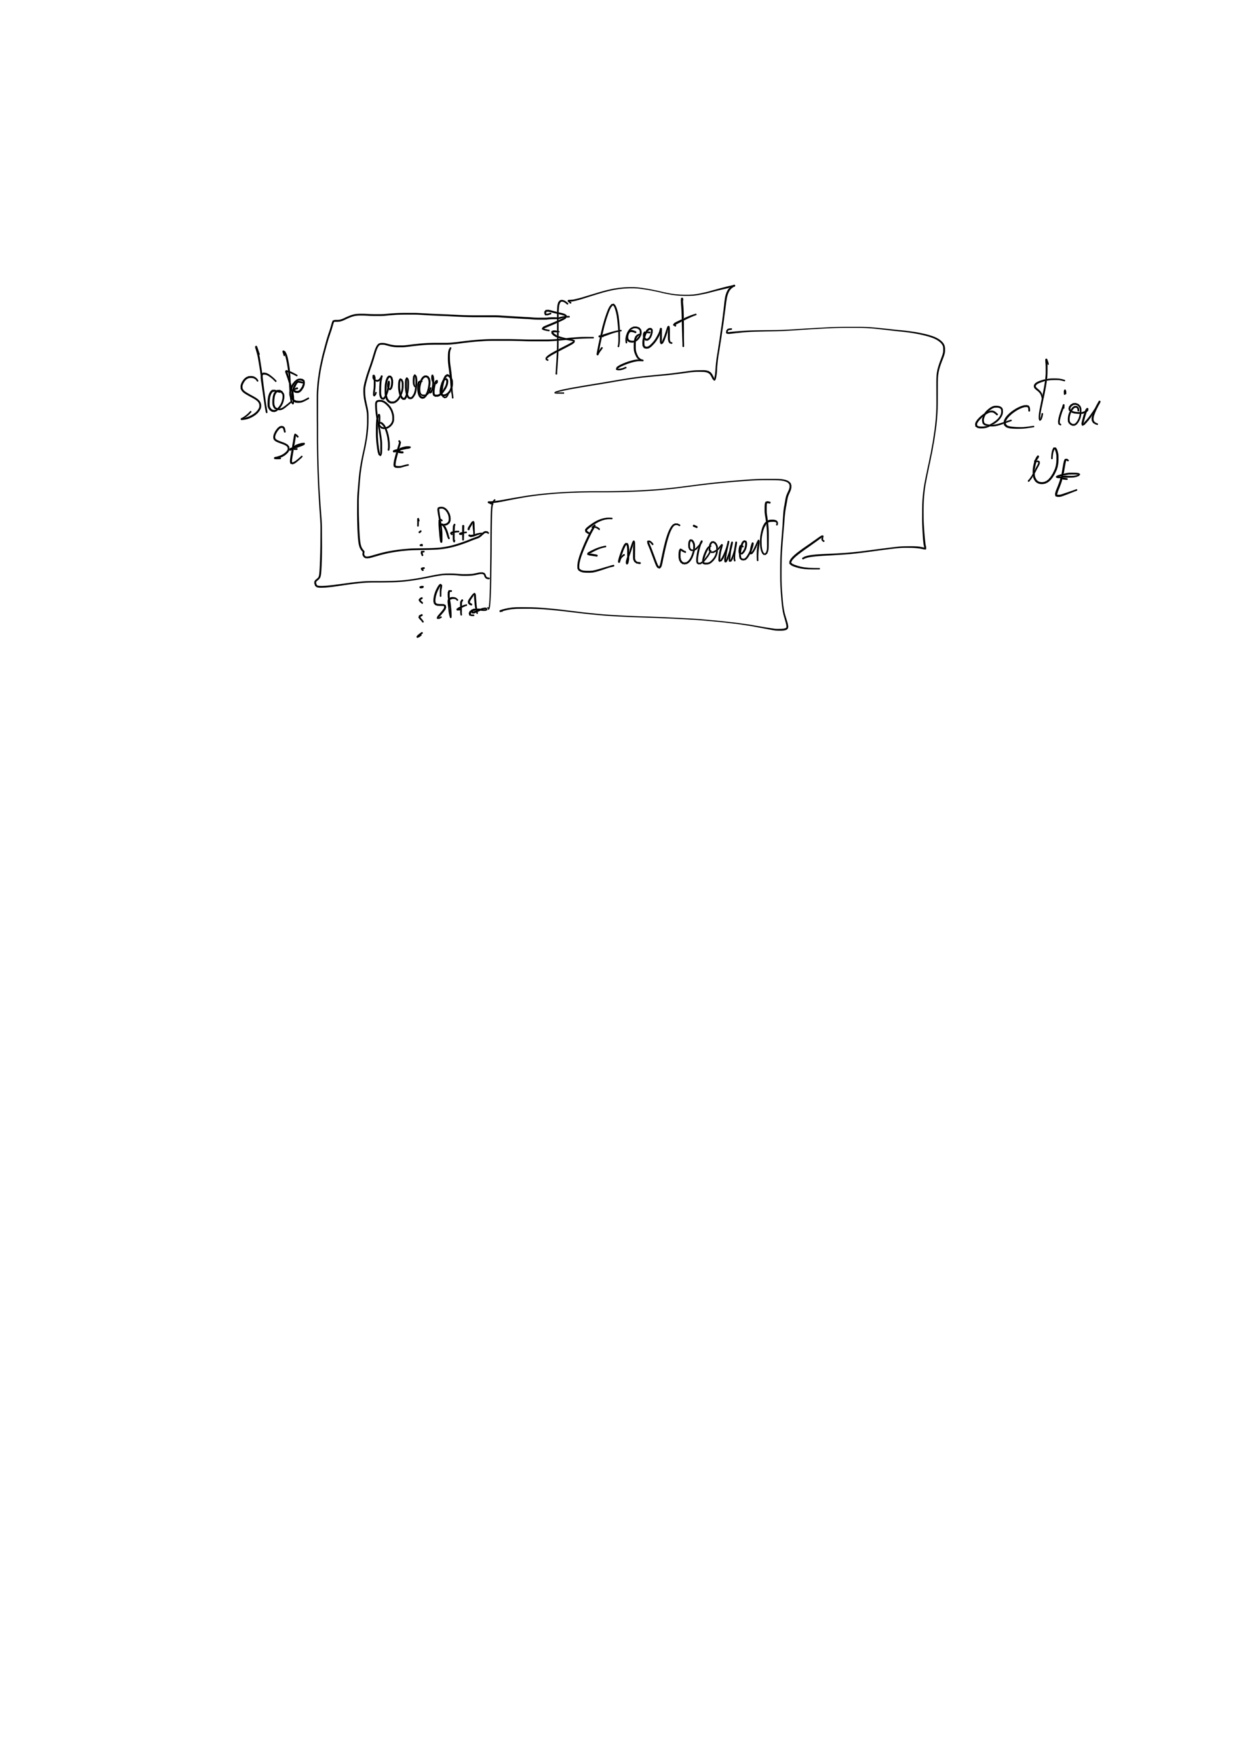
\includegraphics[width=\textwidth]{tex_thesis/figures/ch2/mdp_sketch.pdf}
    \caption{Markov decision process \citep{sutton2018reinforcement}. \todo check on the same page as the Section where it is defined.}
    \label{fig:ch2_mdp}
\end{figure}

We obtain the definition of a Markov decision process (MDP) by considering a single agent in a stochastic game (see Section \ref{sec:ch2_stochastic_Game}).
We define an MDP as a tuple $[\mathcal{S}, \mathcal{U}, R, P, \gamma, p_0]$ where a single agent interacts with its environment as presented in Figure \ref{fig:ch2_mdp}.
The agent observes the state $s_t \in \mathcal{S}$ and selects an action from its action space $u_t \in \mathcal{U}$ with a probability defined by its policy $\pi(u_t|s_t)$.
This selected action leads the agent to a new state $s_{t+1}$ with a probability given by the transition function $P:\mathcal{S} \times \mathcal{S} \times \mathcal{U} \rightarrow [0,1]$.
One must denote here the Markovian property: the next state is a function only of the current state and action.

Along the transition of the state, the agent receives a reward $r_t$ defined by the reward function $R:\mathcal{S} \times \mathcal{S} \times \mathcal{U} \rightarrow \mathbb{R}$.
We define the discounted return of a sequence from time step $t$ to time step $T$ as $G_t= \sum_{j=t}^{T-1} \gamma^j r_{t+j}$.
The goal of the agent is to maximise the expected discounted return, so the expected sum of discounted rewards, over a finite episode $\mathbb{E}_{\pi} \left[\sum_{t=0}^{T-1} \gamma^t r_t \right]$, also denoted $\mathbb{E}_{\pi, p_0}\left[ G_0 \right]$ where $p_0$ is the initial distribution of $s_0$.

\todo{The case of a Nash Equilibrium with a single agent.}
Therefore, it needs to learn an optimal policy $\pi^*=\argmax_\pi \mathbb{E}_{\pi}\left[ G_0 \right]$.
To evaluate a policy, we define the state value function $V^\pi(s) = \mathbb{E}_{\pi}\left[G_t|s_t=s\right]$ and the state action value function $Q^\pi(s, u) = \mathbb{E}_{\pi}\left[G_t|s_t=s, u_t=u\right]$.

Most commonly, two families of methods are identified in RL.
The value-based methods learn a value function and derive the policy from it, while the policy-based methods directly learn a policy.
But before diving into these details, we first discuss the difference when the model is known or not.

\todo{exploration exploitation}

\subsection{Model-based or model-free}
\label{sec:ch2_model_based_vs_model_free}

When finding the optimal policy in an MDP, we distinguish methods based on the knowledge of action outcomes.
Indeed, with the model of the MDP, one can simulate the environment to evaluate policies \citep{sutton2018reinforcement}.
\cite{moerland2023model} defines a model as follows: ``A model is a form of reversible access to the MDP dynamics (known or learned)''.
Knowing the model and finding the optimal solution, or learning the model to find the optimal solution of this model, is referred to as model-based RL.
In opposition, learning by trial and error, without a model, is named model-free RL, and in this manuscript, we focus on model-free RL.
Model-based RL is not the primary focus, and we refer to the work of \cite{moerland2023model} that provides many keys to bridge the gap between RL and planning, between model-based and model-free.
Nevertheless, the following Section introduces dynamic programming, techniques that require a model to compute the optimal policy.
Dynamic programming provides the foundation of model-free methods that will afterwards be introduced.

\todo{Model-based RL, learning P(st+1) is sometimes denoted as the third family of RL.}

\subsection{Dynamic programming}
Dynamic programming \citep{bellman1966dynamic} methods compute the optimal policy given a model of an MDP \citep{sutton2018reinforcement}.
They rely on the property that the value functions $V^{\pi^*}$ and $Q^{\pi^*}$ of the optimal policy ${\pi^*}$ satisfy the Bellman equations $\forall s, u$:
\begin{equation}
\label{eq:ch2_bellmanV}
    V^{\pi^*}(s) = \max_u \mathbb{E}[r_t + \gamma V^{\pi^*}(s_{t+1})| s_t=s, u_t=u]
\end{equation}

\begin{equation}
\label{eq:ch2_bellmanQ}
    Q^{\pi^*}(s, u) = \mathbb{E}[r_t + \gamma \max_{u'} Q^{\pi^*}(s_{t+1}, u') |s_t=s, u_t=u]
\end{equation}

Not going into the details of policy evaluation, policy improvement, policy iteration and value iteration, e.g. presented in \citep{sutton2018reinforcement}, one can find the optimal policy by iteratively evaluating and improving the policy with the value functions.
This can be highlighted by developing the value functions for any policy $\pi$ and $\forall s, u$:
\begin{equation}
\label{eq:ch2_V_2}
\begin{split}
    V^\pi(s)= \mathbb{E}_{\pi}\left[G_t|s_t=s\right] & = \mathbb{E}_{\pi}\left[r_t + \gamma V^\pi(s_{t+1})|s_t=s\right]\\
     & = \sum_{u} \pi(u|s) \sum_{s'} P(s', s, u) (R(s', s, u) + \gamma V^\pi(s'))
\end{split}
\end{equation}

\begin{equation}
\label{eq:ch2_Q_2}
\begin{split}
    Q^\pi(s, u) = \mathbb{E}_{\pi}\left[G_t|s_t=s, u_t=u\right] & = \mathbb{E}_{\pi}\left[r_t + \gamma V^\pi(s_{t+1})|s_t=s, u_t=u \right] \\
    &  = \sum_{s'} P(s', s, u) (R(s', s, u) + \gamma V^\pi(s'))
\end{split}
\end{equation}

In addition to requiring the model knowledge $P$ and $R$, the complexity of these methods increases with the size of the state space, often referred to as the curse of dimensionality, which may limit their usage.
Because of our direction towards model-free RL, without the model knowledge, our interest here is to present Equations \ref{eq:ch2_bellmanV}, \ref{eq:ch2_bellmanQ}, \ref{eq:ch2_V_2} and \ref{eq:ch2_Q_2} that may ease the understanding of the learning concepts.


\subsection{Value-based methods} \label{sec:ch2_value_based_methods}
Value-based methods are designed to learn value functions.
Maybe one of the first methods in model-free RL is Q-learning \citep{watkins1992q}, where the state-action value function learned is the optimal one defined as $Q^{\pi^*}(s, u)=\max_{\pi}Q^\pi(s, u)$.
This enables the agent to greedily select the action $\pi^*(u|s)=\argmax_u Q^{\pi^*}(s, u)$.

Q-learning is classified as a tabular method because it maintains estimations of $Q(s, u)$ in a table, one for each state-action pair.
It updates these estimations based on themselves, also called bootstrapping and is based on temporal difference (TD) learning.
Following the update rule of Equation \ref{eq:ch2_QLearning}, one can repeatedly update the estimation $Q(s, u)$ by adding the temporal difference weighted by a factor $\alpha$ controlling the update size.

\begin{equation}
\label{eq:ch2_QLearning}
    Q(s_t, u_t) \leftarrow Q(s_t, u_t) + \alpha \left[ r_t + \gamma \max_u Q(s_{t+1}, u) - Q(s_t, u_t) \right]
\end{equation}

It is important to denote that this algorithm allows to approximate $Q^{\pi^*}(s, u)$ indepentely of the policy used to sample transitions ($s_t, u_t, r_t, s_{t+1}$).
These transition samples are typically generated with an $\epsilon$-greedy policy, that takes a random action instead of the greedy one with a probability $\epsilon$.
This is a characteristic of the off-policy methods, whereas the on-policy methods improves the policy used to generate the transitions.
In this manuscript, we consider only off-policy value-based methods but on-policy methods are discussed further in Section \ref{sec:ch2_Cooperation}.
To cite one, SARSA is a well-known on-policy value-based method, e.g. in \citep{sutton2018reinforcement}.

With Q-learning, the table size to maintain increases as the state-action space size increases.
Therefore, it can become impractical to compute $Q(s, u)$ for each state-action pair, and it requires function approximators.
There exist various function approximators, but in this manuscript, we restrict ourselves to neural networks.

A neural network is a function $f: \mathcal{X} \rightarrow \mathcal{Y}$ that maps an input ($\in\mathcal{X}$) to an output ($\in\mathcal{Y}$) based on its parameters $\theta$: $y = f(x;\theta)$.
These parameters define a sequence of functions, linear or not.
These functions are differentiable, allowing optimising their parameters by following the gradient of an objective, commonly called a loss function $\mathcal{L}(\theta)$.
To minimise the loss, parameters can be updated by gradient descent: $\theta = \theta - \alpha \nabla \mathcal{L}(\theta)$.
Optimising a neural network is also referred to as training it.
There exist many loss functions to train neural networks, depending on the function to be approximated and nowadays, neural networks are very large, leading to the name of deep learning.
See \citep{zhang2023dive} or \citep{pml1Book} for many more details.
Finally, reinforcement learning with a neural network is called deep reinforcement learning, e.g. in \citep{introDeepRL}.
Hereafter, we introduce how to train such networks to approximate a value function and, in Section \ref{sec:ch2_policy_based_methods}, to approximate a policy.

A standard method in RL, referred to as deep Q-network (DQN) \citep{Mnih2015}, is to approximate $Q(s, u)$ with a neural network $\theta$.
This can be achieved by minimising the loss defined in Equation \ref{eq:ch2_dqnloss} where $B$ is the replay buffer and $\theta'$ is the target network.
The replay buffer $B$ stores transitions $\langle s_{t},u_{t},r_{t},s_{t+1}\rangle$ from which batches of transitions are sampled to update $\theta$ \citep{lin1992self}.
This replay buffer allows updating the neural network with past transitions.
In turns, the target network $\theta'$ is a copy of $\theta$ updated periodically that reduces the moving target problem as $\theta$ is updated several times before updating $\theta'$, e.g., in \citep{Mnih2015}.

\begin{equation}
\label{eq:ch2_dqnloss}
    \mathcal{L}(\theta) = \mathbb{E}_{\langle . \rangle\sim B} \big[\big(r_{t} + \gamma \max_u Q(s_{t+1}, u; \theta')- Q(s_{t}, u_{t}; \theta)\big)^{2}\big]
\end{equation}

In both Equations \ref{eq:ch2_QLearning} and \ref{eq:ch2_dqnloss}, the $max$ operator can introduce some positive bias. 
To overcome this bias, a method called Double Q-learning \citep{hasselt2010double}, and adapted to Q-learning with approximators \citep{van2016deep}, consists in selecting the action that maximises the updated $Q(., \theta)$ to compute the target state-action value.
The loss is therefore adapted as in Equation \ref{eq:ch2_doubleQ}.

\begin{equation}
    \label{eq:ch2_doubleQ}
    \mathcal{L}(\theta) = \mathbb{E}_{\langle . \rangle\sim B} \big[\big(r_{t} + \gamma Q(s_{t+1}, \argmax_u Q(s_{t+1}, u;\theta) ; \theta')- Q(s_{t}, u_{t}; \theta)\big)^{2}\big]
\end{equation}

Double Q-learning is one of the possible improvements of DQN, and we refer to the Rainbow paper \citep{hessel2018rainbow} that addresses several others.
To cite one, the extension to distributional RL, which approximates distributions instead of expected returns, can be of interest \citep{bellemare2017distributional, THEATE2023199}. 

\subsection{Policy-based methods} \label{sec:ch2_policy_based_methods}
Policy-based methods are designed to learn the policy.
In this manuscript, we restrict to the subclass of policy gradient methods where a neural network parametrised by $\theta$ approximates a differentiable policy $\pi_\theta=\pi(u|s;\theta)$.
Policy gradient methods hence update $\theta$ to find the optimal policy that maximises the expected return denoted as  $J(\pi_\theta) = \mathbb{E}_{\pi_\theta}[G_0]$.
Maybe one of the first method is REINFORCE \citep{williams1992simple} which updates $\theta$  by ascending the gradient given in Equation \ref{eq:ch2_reinforce_grad}: $\theta = \theta + \alpha \nabla_\theta J(\pi_\theta)$.

\begin{equation}
\label{eq:ch2_reinforce_grad}
    \nabla_\theta J(\pi_\theta) = \nabla_\theta \mathbb{E}_{\pi_\theta}[G_0] = \mathbb{E}\left[\sum_{t=0}^{T-1} Q(s_t, u_t) \nabla_\theta \log \pi(u_t|s_t;\theta)\right]
\end{equation}

Estimating $Q(s_t, u_t)$ instead of computing it is a solution proposed by the actor-critic methods \citep{sutton1999policy,konda1999actor}.
This type of method expands upon REINFORCE by incorporating a second neural network, called the critic and denoted by $\phi$, that estimates $Q(s_t, u_t;\phi)$ while the actor is the parametrised policy $\pi(u|s;\theta)$.
The new loss provided by incorporating the critic is given in Equation \ref{eq:ch2_reinforce_grad}.
\begin{equation}
\label{eq:ch2_Q_actor_crit}
    \nabla_\theta J(\pi_\theta) = \mathbb{E}\left[\sum_{t=0}^{T-1} Q(s_t, u_t;\phi) \nabla_\theta \log \pi(u_t|s_t;\theta)\right]
\end{equation}

Moreover, a baseline can be injected into the gradient to reduce variance.
Usually, the baseline is  $V(s)$, independent of the action taken, and $Q(s, u;\phi)$ is replaced by the advantage function $A(s,u; \phi)$ \citep{10.5555/2074022.2074088}, leading to the gradient expressions of Equation \ref{eq:ch2_baseline_actor_crit}:

\begin{align}
\begin{split}
\label{eq:ch2_baseline_actor_crit}
    \nabla_\theta J(\pi_\theta)
    & = \mathbb{E}\left[\sum_{t=0}^{T-1} [Q(s_t, u_t) - V(s_t)] \nabla_\theta \log \pi(u_t|s_t;\theta)\right]\\
    & = \mathbb{E} \left[\sum_{t=0}^{T-1} A(s_t, u_t; \phi) \nabla_\theta \pi(s_t, u_t; \theta)\right]
\end{split}
\end{align}

Estimating the advantage with only one neural network is possible either by $A(s_t,u_t; \phi)=Q(s_t, u_t;\phi)-\sum_u \pi(u|s_t;\theta) Q(s_t,u; \phi)$ or by $A(s_t,u_t; \phi)=r_t +\gamma V(s_{t+1};\phi) - V(s_t;\phi)$.
This critic can be trained on-policy or off-policy following methods described in Section \ref{sec:ch2_value_based_methods}.
This is why actor-critic methods are sometimes described as a mix between value-based and policy-based methods.

Nowadays, advanced policy-based methods relying on the actor-critic paradigm appear to be the most successful.
We can cite trust region policy optimisation (TRPO) \citep{schulman2015trust} and its variant proximal policy optimisation (PPO) \citep{schulman2017ppo}.
Both of these methods rely on a controlled policy update by constraining the loss of REINFORCE defined in Equation \ref{eq:ch2_reinforce_grad}.

\section{Partial observability} \label{sec:ch2_partial_observability}
As defined in previous Sections, the Markov decision process and the stochastic game are fully observable.
Agents have complete access to the state environment and perceive everything without uncertainty.
In real-world applications, it is not always possible to consider this feasible.
Anyone can come up with ideas of a partially observable environment.
Especially given our definition of agents ``acting upon information it perceives'': the information about the state of the environment can be uncertain.

Starting with SARL, when the agent can only partially perceive the state, the MDP is said to be a partially observable Markov decision process (POMDP) \citep{KAELBLING199899}. 
The MDP definition of Section \ref{sec:ch2_mdp} is adapted easily to the POMDP by adding an observation space $\mathcal{Z}$ and an observation function $O:\mathcal{S} \times \mathcal{Z} \rightarrow [0, 1]$, mapping a state and an observation to the probability of observing the latest.
As a consequence, the agent's policy $\pi$ cannot be a function of the state anymore.
But it could be a function of the observation.
Doing so can be a bad idea, because the observation does not respect the Markovian property defined in Section \ref{sec:ch2_mdp}.
This why, in POMDP, the decision is made based on the history of past observations and action s $(\mathcal{Z} \times \mathcal{U})^\tau$, denoted as $\tau$.
We therefore denote the policy as $\pi(u_t|\tau_t,o_t): (\mathcal{Z} \times \mathcal{U})^t \rightarrow [0,1]$.

In practice, history can become very large, which can be impractical.
The agent then maintains a belief $b(s)=Pr(s|\tau,o)$, the probability of being in a given state, knowing the history of observations and spaces.
To approximate this belief, it is possible to benefit from recurrent neural networks (RNN).
Several types of recurrent cells exist, such as GRU \citep{Chung2014EmpiricalModeling} or LSTM \citep{Hochreiter1997LongMemory}.
These networks maintain a hidden state, updated at each timestep, which can be considered as a memory.
Recurrent networks have many applications, and in POMDP, their hidden state allows maintaining a belief without processing the whole history at each timestep.
Using recurrent networks to compute policies is thus a common practice in POMDP, resulting in recurrent policies.
Adding RNN has demonstrated convincing results, such as in recurrent policy gradients or \citep{wierstra2010recurrent} or in deep recurrent Q-network (DRQN) \citep{Hausknecht2015DeepMDPs}.
We suggest that readers interested in details read the pedagogical paper of \cite{lambrechts2022recurrent}.
This paper demonstrates that the correlation between the hidden state of RNNs, used to approximate policies, and the belief increases as the training progresses.

When considering multi-agent, the same changes can be applied to the stochastic game definition, leading to partially observable stochastic games (POSG).
We thus need to add a set of $n$ observation spaces $\mathcal{Z}$ and a set of $n$ observation function $O$.
When agents are all the same, we can consider that both sets are singleton, which is sometimes a shortcut taken in the literature.
Finally, as detailed in \citep{DecPomdp}, the belief cannot be considered similarly in multi-agent systems.
Because in MARL, being in a given state is not only a function of one agent's history, it is a function of all agents' history.
This manuscript does not address multi-agent belief, and we refer to \citep{DecPomdp} for more details \todo{check albrechts book}.
In a POSG, we consider that an agent's policy is a function $\pi^{a}(u_t^{a}|\tau_t^{a},o_t^{a}): (\mathcal{Z}^a \times \mathcal{U}^a)^t \rightarrow [0,1]$, which maps its history $\tau_t^{a} \in (\mathcal{Z}^a \times \mathcal{U}^a)^{t-1}$ and its current observation $o_t^{a}$ to the probability of taking action $u_t^{a}$.
We also consider that this policy is recurrent.


\todo{check queue less exposant a ou subscript a sont les mêmes partout.}\cleardoublepage
\part{Learn to cooperate}\label{part:coop}
\chapter{Cooperation}\label{ch:cooperation}\cleardoublepage
\chapter{The Deep Quality-Value family in Dec-POMDP}\label{ch:qvmix}
\begin{chapter_outline}

This chapter presents four value-based methods issued from the Deep Quality-Value (DQV) family for the Dec-POMDP framework.
We introduce the DQV family and detail the contribution of this chapter in Section~\ref{sec:ch4_intro}.
We then formally define DQV and the four methods in Section~\ref{sec:ch4_methods}.
The experimental setup to evaluate them is presented in Section~\ref{sec:ch4_experiments}, followed by the corresponding results in Section~\ref{sec:ch4_results}.
This chapter ends with a conclusion in Section~\ref{sec:ch4_conclusion}.

This chapter is an adapted version of the publication \citep{leroy2020qvmix} \textit{QVMix and QVMix-Max: extending the deep quality-value family of algorithms to cooperative multi-agent reinforcement learning}, P. Leroy, D. Ernst, P. Geurts, G. Louppe, J. Pisane, and M. Sabatelli. AAAI-21 Workshop on Reinforcement Learning in Games, 2021.

\end{chapter_outline}


\section{Introduction} \label{sec:ch4_intro}

This chapter introduces four methods to learn to cooperate in a Dec-POMDP, defined in Section~\ref{sec:ch3_decpomdp}.
They are adapted from the Deep Quality-Value (DQV) family of algorithm \citep{sabatelli2020deep}.
DQV methods jointly learn an approximation of the state-value function $V$ alongside an approximation of the state-action value function $Q$.
They have proven to significantly outperform popular algorithms in SARL, such as DQN and DDQN defined in Section~\ref{sec:ch2_value_based_methods}.
The four methods follow two modes of training and execution in a Dec-POMDP, introduced in Section~\ref{sec:ch3_intro}.
The methods designed for the decentralised mode are called IQV and IQV-Max.
The other two dedicated to the CTDE mode are called QVMix and QVMix-Max.
They are tested with the StarCraft Multi-Agent Challenge (SMAC) suite of environments, introduced in Section~\ref{fig:ch3_smac}.
They are compared with IQL, QMIX and MAVEN, three value-based methods in multi-agent reinforcement learning defined in Section~\ref{sec:ch3_value}.

Finally, the contributions of \citep{leroy2020qvmix} presented in this chapter can be divided into three parts.
The first is the generalisation of the DQV family of algorithms to cooperative MARL problems, their performance in the decentralised mode and their fundamental limitations.
The second is the introduction of two methods, QVMix and QVMix-Max.
Both combine the original benefits of the DQV algorithms with CTDE, resulting in a better performance than state-of-the-art techniques of their time.
The third is to link their better performance to the overestimation bias of the $Q$ function that characterises model-free RL algorithms.

\section{Methods} \label{sec:ch4_methods} 

As introduced, the work presented in this chapter revolves around the Deep Quality-Value (DQV) family of DRL algorithms \citep{sabatelli2018deepQV, sabatelli2020deep}.
These SARL techniques learn an approximation of the state value function $V$ alongside an approximation of the state-action value function $Q$.
The DQV algorithms extend the tabular RL algorithms called QV($\lambda$) learning \citep{wiering2005qv, wiering2009qv} with neural networks as function approximations.
There are two possible ways of learning a joint approximation of the $V$ function, $V(s;\phi)\approx V^{\pi^*}(s)$, and of the $Q$ function, $Q(s, u;\theta)\approx Q^{\pi^*}(s, u)$.

DQV learns an approximation of the $V$ function by minimising
\begin{equation}
    \mathcal{L}(\phi) = \mathbb{E}_{B} \bigg[\big(r_{t} + \gamma V(s_{t+1}; \phi') - V(s_{t}; \phi)\big)^{2}\bigg],
    \label{eq:ch4_dqv_v_update}
\end{equation} 
while the $Q$ function is learned by minimising 
\begin{equation}
    \mathcal{L}(\theta) = \mathbb{E}_{B} \bigg[\big(r_{t} + \gamma V(s_{t+1}; \phi')  - Q(s_{t}, u_{t}; \theta)\big)^{2}\bigg].
\label{eq:ch4_dqv_q_update}
\end{equation}
    
DQV-Max learns the $Q$ function with the same loss defined in Equation \eqref{eq:ch4_dqv_q_update} but learns the $V$ function by minimising
\begin{equation}
        \mathcal{L}(\phi) = \mathbb{E}_{B} \bigg[\big(r_{t} + \gamma \: \underset{u\in \mathcal{U}}{\max}\: Q(s_{t+1}, u; \theta') - V(s_{t}; \phi)\big)^{2}\bigg].
        \label{eq:ch4_dqv_max_v}
\end{equation}
As in DQN, the replay buffer $B$ stores transitions $\langle s_{t},u_{t},r_{t},s_{t+1}\rangle$ from which batches of transitions are sampled to update the networks.
The target network $\theta'$ and $\phi'$ are a copies of $\theta$ and $\phi$ updated periodically.

The extension to the decentralised MARL methods is straightforward, like IQL from DQN.
This leads to IQV and IQV-Max using, respectively, the DQV and DQV-Max update rules to learn $Q_a(\tau^a, u^a;\theta)$ and $V_a(\tau^a;\phi)$ independently.
For the CTDE mode, the methods are QVMix and QVMix-Max, and they follow the DQV and DQV-Max update rules to learn $Q^{mix}_{tot}(s, \mathbf{u})$.
The architecture of the $Q_a$ and the mixer network is the same as in QMIX, using exactly the same monotonic decomposition.
In both QVMix and QVMix-Max, the $V$ network computes a central state value function $V^{mix}_{tot}(s)$ as a function of individual $V_a(\tau^a;\theta)$.
It has the same architecture as the $Q$ ones of QMIX, except they have a single output. 
The architecture is presented in Figure~\ref{fig:ch4_qvmix}.
In QVMix, $V^{mix}_{tot}$ is updated following the loss defined in Equation~\ref{eq:ch4_dqv_v_update} and with the loss defined in Equation~\ref{eq:ch4_dqv_max_v} for QVMix-Max.
Individual networks are GRU, and $B$ stores sequences of contiguous transitions instead of single transitions to train recurrent neural networks.

\begin{figure}
\centering

\begin{tikzpicture}[node distance=.5cm]

\tikzstyle{netbox} = [rectangle, rounded corners, minimum width=1cm, minimum height=1cm, draw=blue]
\tikzstyle{mixerbox} = [rectangle, rounded corners, minimum width=4.5cm, minimum height=1.5cm, draw=blue]
\tikzstyle{indixQbox} = [rectangle, rounded corners, minimum width=1.3cm, minimum height=2cm, draw=red]
\tikzstyle{io} = [minimum width=0.2cm,minimum height=0.5cm]
\tikzstyle{emptynetbox} = [rectangle, rounded corners, minimum width=1cm, minimum height=1cm]

\node (output_node) [io] {$V_{mix}^{tot}(s_t)$};
\node (mixerbox) [mixerbox, below=of output_node, yshift=-0cm, label={[xshift=-1.4cm, yshift=-1cm]$Mixer$}] {};
\node (indivQbox1) [indixQbox, below=of mixerbox, xshift=-1.2cm, yshift=-.5cm, label={[xshift=-0.22cm, yshift=.2cm]$V_{a_1}(\tau^1_t)$}] {$V_{a_1}$};
\node (indivQboxn) [indixQbox, below=of mixerbox, xshift=1.2cm, yshift=-.5cm, label={[xshift=0.22cm, yshift=.2cm]$V_{a_n}(\tau^n_t)$}] {$V_{a_n}$};
\node (mixer_net) [netbox, below=of output_node, yshift=-0.3cm] {$h_o$};
\node (param_net) [netbox, right=of mixer_net] {$h_p$};
\node (param_net2) [emptynetbox, left=of mixer_net] {};

\node (intput_node1) [io,below=of indivQbox1, yshift=-0cm, label={[xshift=1.2cm, yshift=1.2cm]. . .}] {$o^{a_1}_t$};
\node (intput_noden) [io,below=of indivQboxn, yshift=-0cm] {$o^{a_n}_t$};
\node (intput_nodestate) [io, right=of param_net] {$s_t$};
\node (intput_nodestate2) [io, left=of param_net2] {};

\draw [-Latex, thick] (intput_node1) -- (indivQbox1);
\draw [-Latex, thick] (intput_noden) -- (indivQboxn);
\draw [-Latex, thick] (indivQbox1) --  (mixer_net);
\draw [-Latex, thick] (indivQboxn) -- (mixer_net);
\draw [-Latex, thick] (param_net) -- (mixer_net) node[midway, yshift=0.3cm] {$|.|$};
\draw [-Latex, thick] (intput_nodestate) -- (param_net);
\draw [-Latex, thick] (mixer_net) -- (output_node);

%\draw[thick, rounded corners, draw=blue, fill=blue!50, opacity=0.2] ($(mixerbox.north west)+(-0.5,0.5)$) rectangle ($(indivQboxn.south east)+(1,-0.5)$);
\draw[thick, rounded corners, draw=red, fill=red!50, opacity=0.2] ($(indivQbox1.north west)$) rectangle ($(indivQbox1.south east)$);
\draw[thick, rounded corners, draw=red, fill=red!50, opacity=0.2] ($(indivQboxn.north west)$) rectangle ($(indivQboxn.south east)$);
\end{tikzpicture}
\caption{Architecture of the $V_{mix}$ network.}
\label{fig:ch4_qvmix}
\end{figure}

\todo{read Matthia thesis to add more?}

\section{Experiments} \label{sec:ch4_experiments}

Our experiments evaluate seven methods in total.
The four defined in this chapter, QVMix, QVMix-Max, IQV and IQV-Max and the three forming the state of the art at that time, QMIX, MAVEN and IQL, defined in Chapter~\ref{ch:cooperation}.
As a test-bed, we use SMAC and evaluate the methods on eight different maps: \texttt{3m}, \texttt{8m}, \texttt{so\_many\_baneling}, \texttt{2m\_vs\_1z}, \texttt{MMM}, \texttt{2s3z}, \texttt{3s5z} and \texttt{3s\_vs\_3z}. 
We refer the reader to Section~\ref{sec:ch3_smac} for the details on SMAC.
It is worth noting that the maps chosen for our experiments differ in complexity. 
In SMAC, the goal is to maximise the sum of discounted rewards achieved by reducing each opponent team unit's health to zero, called a win.

Each method is executed on every map ten times, and neural networks are trained from scratch each time.
Networks are trained for $5m$ timesteps for the first four maps mentioned above and $10m$ timesteps for the four others, chosen because of the time required to achieve convergence.
Every $20.000$ timestep, the parameters of the networks are saved to perform $24$ testing episodes.

Each algorithm uses the same hyperparameter values to compare the tested method fairly.
Specifically, we refer to the authors of QMIX, MAVEN, and IQL to determine the hyper-parameters set and keep the same values for QVMix, QVMix-Max, IQV, and IQV-Max. 
For a more thorough presentation of all used hyper-parameters, we refer the reader to the open-sourced code\footnote{\url{https://github.com/PaLeroy/QVMix}}.
As is common practice within the literature, the individual networks' parameters are shared among agents to improve the algorithms' learning speed.
This means a single individual $Q_a$ network is used for all agents.
A one-hot encoding of the agent id ($\{1,..,n\}$) is added to the observation space to allow individual networks to produce different policies per agent.

\section{Results} \label{sec:ch4_results}
We report the results of experiments in two different ways.
We start by analysing each tested method's win rate before investigating the quality of the value functions learned by all algorithms.

The means of win rate for each map and algorithm are reported in Table~\ref{tab:main_results}. 
Suppose the algorithms perform equally in terms of overall performance, meaning the average win rate is the same. 
In that case, we consider the one which significantly converges the fastest to be the best-performing algorithm.
Please note that reporting an episode's win rate is a good indicator of the quality of an agent's learned policy since, as introduced in the previous section, a win directly corresponds to the best achievable sum of rewards an agent can receive.

\begin{table*}
    \centering
    \setlength\tabcolsep{4.5pt}
\begin{tabular}{cccccccc}
        \toprule
        
        Map & QMIX & MAVEN &     QVMix & QVMix-Max  & IQL & IQV & IQV-Max\\
        \midrule
         \texttt{3m} & \underline{100} & 98.7 &   \textbf{100} & 100 & 93.3 & 93.3& 96.6 \\
        %\hline
        
         \texttt{8m} & 96.6& \underline{98.3} &  \textbf{100} & 96.6 & 83.3& 93.3& 90\\
        %\hline
        
         \texttt{so\_many\_baneling} & \underline{100} & 97  & \textbf{100}& 100& 50 & 40 & 40\\
        %\hline
        
        \texttt{2m\_vs\_1z} & \underline{100} & 100 &\textbf{100} & 96.6  & 100 & 100 & 100\\
        \midrule
        
       \texttt{MMM} & \textbf{100} & \underline{97.0} & 93.3 & 96.6  & 61.6 & 83.3 & 50 \\
        %\hline
        
        \texttt{2s3z}  & 96.6 & \underline{97.5} &  96.6 & \textbf{100} & 59.9 & 56.6 & 40 \\
        %\hline
        
        \texttt{3s5z} & 40 & 40.8 &\textbf{86.6} & \underline{43.3}  & 16.6 & 13.3 & 0 \\
        %\hline
        
        \texttt{3s\_vs\_3z}  & \underline{100} & 97.9  &  \textbf{100} & 100  & 83.3 & 76.6 & 63.3 \\
        \bottomrule
    \end{tabular}
    
% \begin{subtable}{\linewidth}
% \centering
% \begin{tabular}{|c|c|c|c|c||c|c|c|}
%         \hline
%         Map & QMIX & MAVEN &     QVMix & QVMix-Max  & IQL & IQV & IQV-Max\\
%         \hline
%         \texttt{3m} & \underline{}100 & 98.7 &   bf100 & 100 & 93.3 & 93.3& 96.6 \\
%         %\hline
        
%          \texttt{8m} & 96.6& \underline{}98.3 &  bf100 & 96.6 & 83.3& 93.3& 90\\
%         %\hline
        
%          \texttt{so\_many\_baneling} & \underline{}100 & 97  & bf100& 100& 50 & 40 & 40\\
%         %\hline
        
%          \texttt{2m\_vs\_1z} & \underline{}100 & 100 &bf100 & 96.6  & 100 & 100 & 100\\
%         \hline
% \end{tabular}
% \subcaption[]{5m training timesteps.}
% \end{subtable}%

% \begin{subtable}{1\linewidth}
% \centering
% \begin{tabular}{|c|c|c|c|c||c|c|c|}
%         \hline
%         Map & QMIX & MAVEN &     QVMix & QVMix-Max  & IQL & IQV & IQV-Max\\
        
%             \hline
%        \texttt{MMM} & bf100 & \underline{}97.0 & 93.3 & 96.6  & 61.6 & 83.3 & 50 \\
%         %\hline
        
%         \texttt{2s3z}  & 96.6 & \underline{}97.5 &  96.6 & bf100 & 59.9 & 56.6 & 40 \\
%         %\hline
        
%         \texttt{3s5z} & 40 & 40.8 &bf86.6 & \underline{}43.3  & 16.6 & 13.3 & 0 \\
%         %\hline
        
%         \texttt{3s\_vs\_3z}  & \underline{}100 & 97.9  &  bf100 & 100  & 83.3 & 76.6 & 63.3 \\
%         \hline
% \end{tabular}
% \subcaption[]{10m training timesteps.}
% \end{subtable}


    \caption{
    Means of win rates achieved in eight scenarios at the end of training by QMIX, MAVEN, QVMix, QVMix-Max, IQL, IQV, and IQVMax. 
    In the first four scenarios, \texttt{3m}, \texttt{8m}, \texttt{so\_many\_baneling} and \texttt{2m\_vs\_1z}, it is measured after $5$ millions training timesteps.
    In the last four, \texttt{MMM}, \texttt{2s3z}, \texttt{3s5z} and \texttt{3s\_vs\_3z} it is measured after $10$ millions training timesteps.
    We report the best and second-best means by \textbf{bolding} and \underline{underlining} them. When results are equivalent, the cells report the fastest and second-fastest method that reaches a win-rate of $100\%$ as shown in Figure~\ref{fig:all_win_curves}.}
    \label{tab:main_results}
\end{table*}

We start by observing the differences in performance between the decentralised mode methods IQL, IQV, and IQV-Max and their respective CTDE extensions QMIX, QVMix, QVMix-Max, and MAVEN.
As one might expect, we can see from the results reported in Figure~\ref{fig:ch4_2m1zwin} that methods for the decentralised mode converge slowly when compared to their CTDE counterparts on the considered \texttt{2\_vs\_1z} map.
This is particularly interesting since it shows that the DQV family of algorithms can be successfully adapted to MARL, both in the decentralised mode and in the CTDE one.
However, these results are challenged once the number of agents in the maps increases: examples of such maps are \texttt{so\_many\_baneling}, \texttt{MMM} or \texttt{3s5z}.
The performance of decentralised methods starts to drop, highlighting that CTDE methods learn faster once the complexity of the training scenario increases, as is clearly reported both in Table~\ref{tab:main_results} and in Figure~\ref{fig:all_win_curves}, where the evolution of the win rate of each algorithm on every tested map is presented.

\begin{figure}
\centering
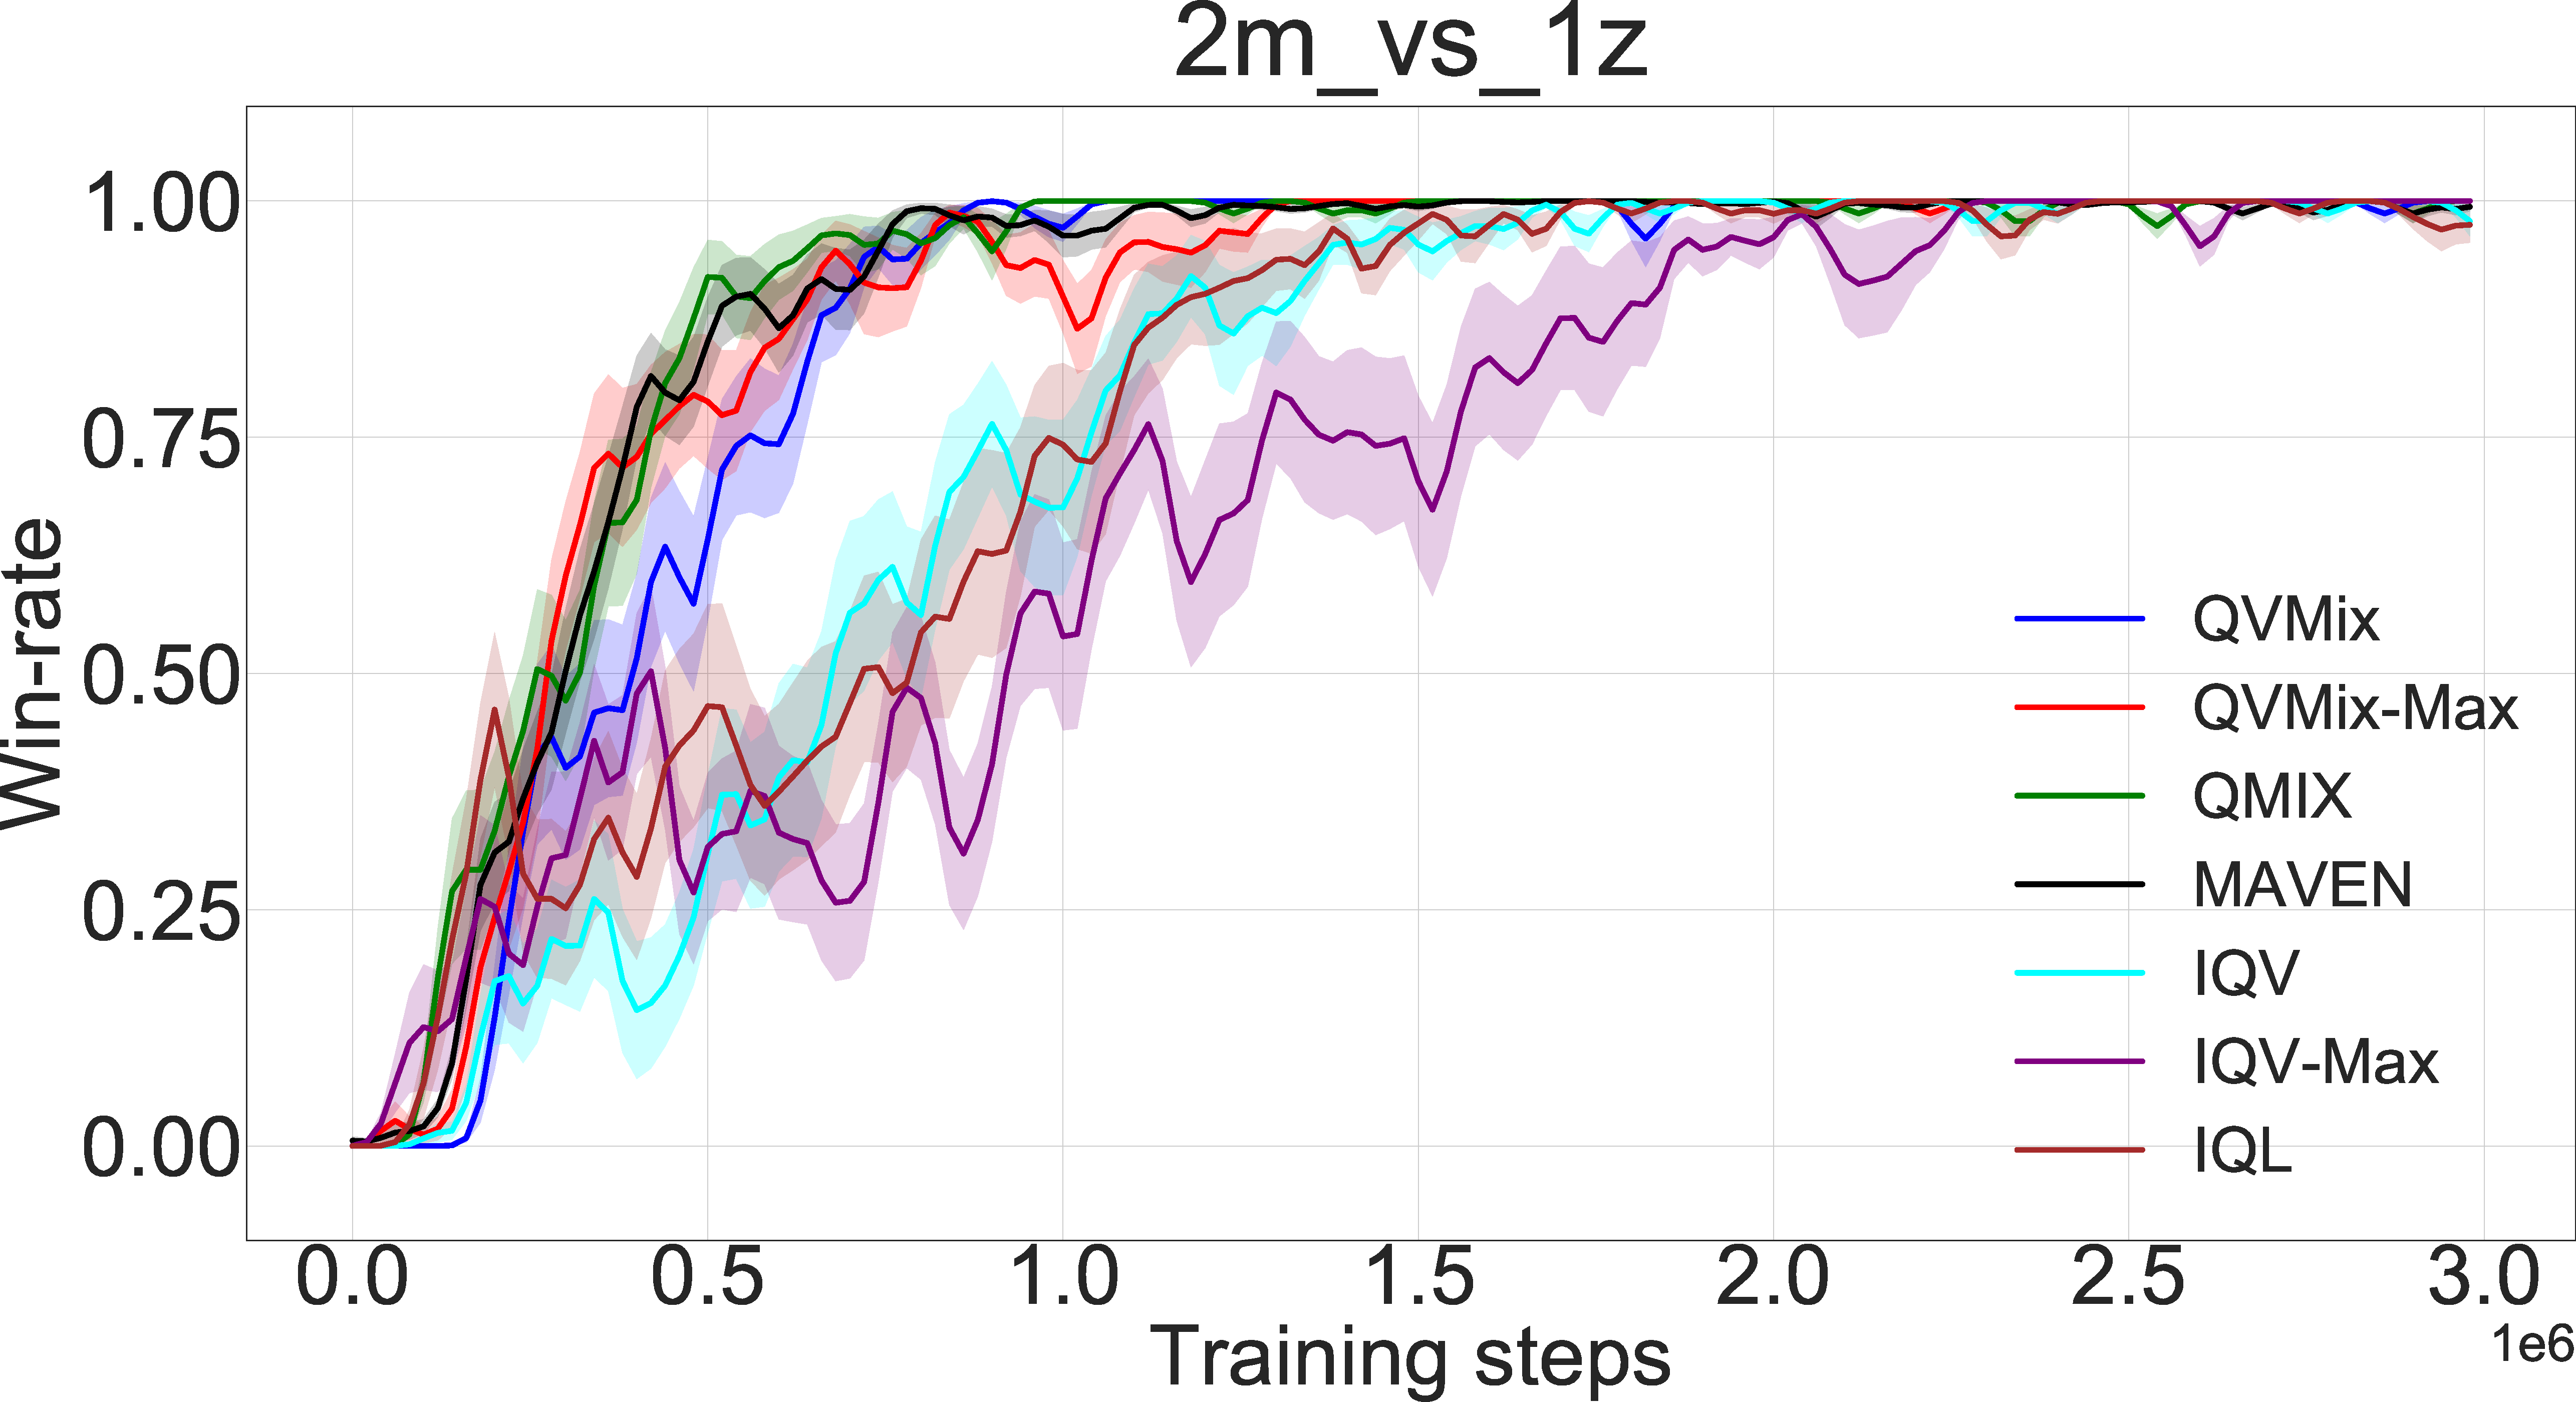
\includegraphics[width=.8\linewidth]{tex_thesis/figures/ch4/2m1zall.pdf}
\caption{Mean of win rates achieved in the \texttt{2m\_vs\_1z} map by QVMix, QVMix-Max, QMIX, MAVEN, IQV, IQVMax and IQL. The error band is proportional to the variance of the measure. We observe that all CTDE methods result in faster training than decentralised ones. All four novel algorithms based on the DQV algorithms can be successfully used in cooperative MARL.}
\label{fig:ch4_2m1zwin}
\end{figure}

\begin{figure*}
\centering
\includegraphics[width=.95\linewidth]{tex_thesis/figures/ch4/all_win.pdf}
\caption{Means of win-rates achieved by QVMix, QVMix-Max, QMIX, MAVEN, IQV, IQVMax and IQL in eight scenarios. Top to bottom, left to right, the scenarios are \texttt{3m}, \texttt{8m}, \texttt{so\_many\_baneling}, \texttt{2m\_vs\_1z}, \texttt{MMM}, \texttt{2s3z}, \texttt{3s5z} and \texttt{3s\_vs\_3z}. The error band is proportional to the variance of win-rates.}
\label{fig:all_win_curves}
\end{figure*}

Therefore, directing attention to CTDE methods, we observe that only QVMix and QVMix-Max perform as well as QMIX and MAVEN in most of the eight maps.
When we consider the \texttt{MMM}, \texttt{3m}, \texttt{2m\_vs\_1z} and the \texttt{so\_many\_baneling} maps, we observe that there is no significant difference between the performance that is obtained by our algorithms and that of QMIX and MAVEN. 
All methods converge towards the best possible winning rate and, in terms of convergence speed, perform closely.

However, when considering the \texttt{2s3z}, \texttt{3s5z} and \texttt{8m} maps, we observe that the performance of QVMix results in even faster learning. 
Of greater interest, when looking at the results obtained on the \texttt{3s5z} map, QVMix is the only algorithm approaching the best possible win rate.
It is also worth noting that the performance of QVMix-Max is always competitive with the one obtained by QVMix, QMIX and MAVEN.
These results are not surprising since a similar performance was observed when DQV-Max was tested in a SARL set-up by \cite{sabatelli2020deep}.

\begin{figure*}
\centering
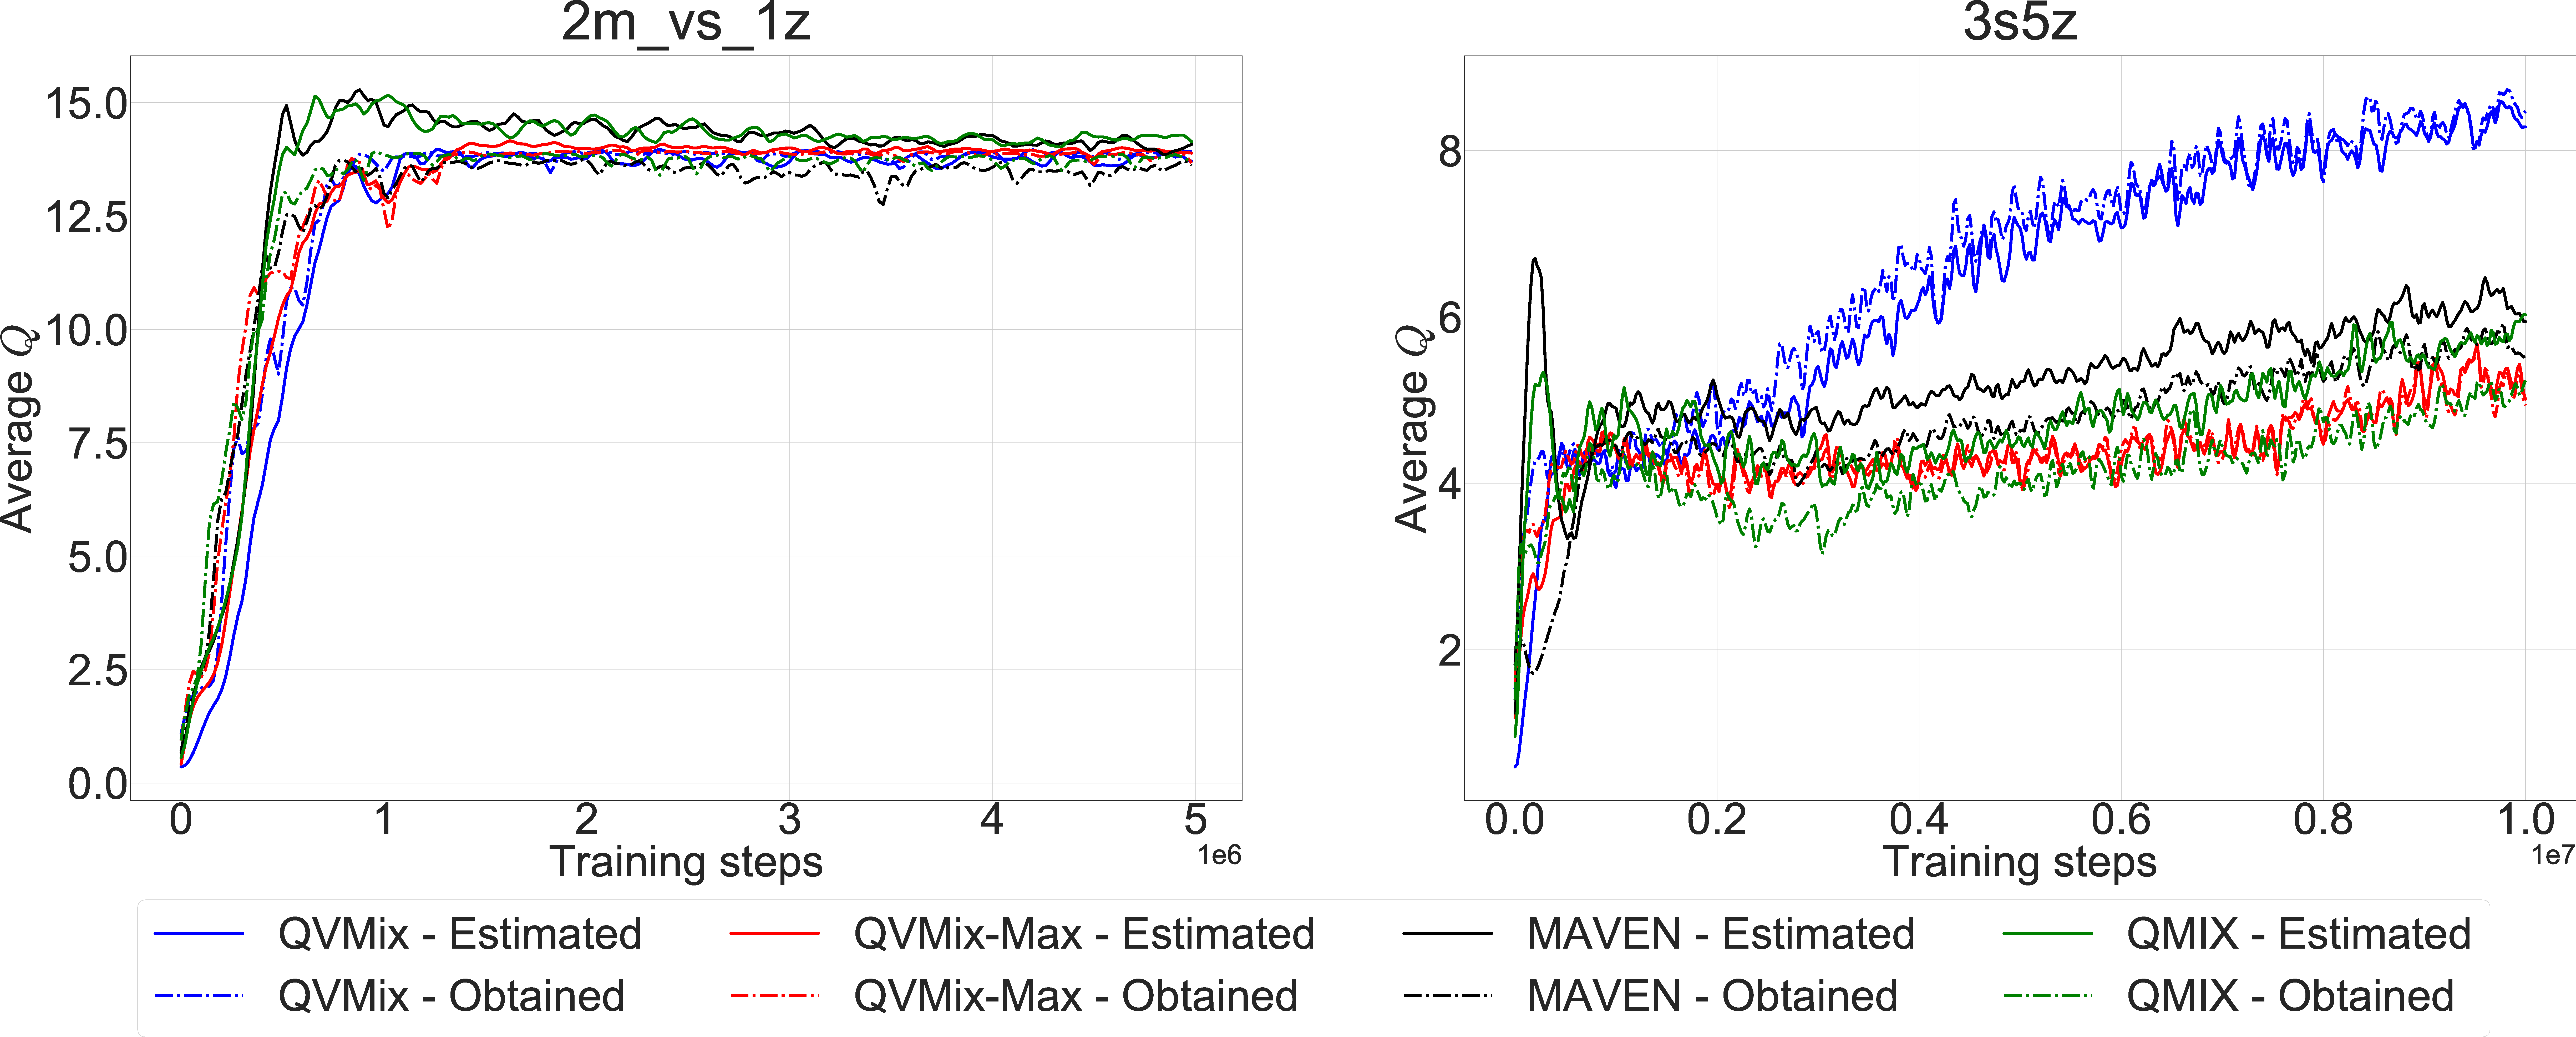
\includegraphics[width=.95\linewidth]{tex_thesis/figures/ch4/2m1z3s5zQ.pdf}
\caption{$Q$ values obtained and estimated when training QVMix, QVMix-Max, MAVEN and QMIX. Dash-dotted lines represent the obtained $Q$ values while solid lines represent the estimated ones.}
\label{fig:exp_plots_overestim:q_best_worse}
\end{figure*}

To understand the reasons behind why QVMix is the best performing algorithm overall, we analyse how well each method estimates the state-joint-action value function $Q_{mix}^{tot}(s_t, \mathbf{u_t})$. 
Since, in most maps, decentralised methods do not perform as well as CTDE methods, we restrict our analysis to CTDE algorithms only where their respective mixer networks give the estimated $Q(s_t, \mathbf{u_t})$.
Since the state space of the maps provided by the SMAC environment is not finite, it is not impossible to compute the exact $Q_{tot}(s_t, \mathbf{u_t})$ for all states to compare them with the estimations.
To overcome this problem, we compute the discounted sum of rewards obtained with the current policy in each visited state during an episode and compare the results with the value function inferred from the $Q_{tot}$ values estimated by the mixer network for these states.
The closer the estimates are to the real $Q(s_t, \argmax_{\mathbf{u}}(Q(s_t,\mathbf{u})))$, the more accurate the learned value function is.

For this experiment, we selected two different maps: the \texttt{2m\_vs\_1z} map, which corresponds to the map on which the best results have been achieved by all methods at the same time, and the \texttt{3s5z} map, which on the other hand, is the map on which QVMix, and others, performed less well.
In Figure~\ref{fig:exp_plots_overestim:q_best_worse}, we report the averaged estimated $Q$ values, represented by the solid lines, and the actual discounted sum of rewards, represented by the dash-dotted lines.
All are computed for each visited state at testing time.
In both scenarios, we can observe that the $Q$ values estimated by QMIX and MAVEN suffer from the overestimation bias of the $Q$ function, while this is not the case for QVMix and QVMix-Max.
Therefore, we justify the better quality of QVMix and QVMix-Max policies by better approximating the $Q$ functions.
However, further work is required to understand this phenomenon in more detail.

\section{Discussion and future work} \label{sec:ch4_conclusion}

In this chapter, we introduced four new value-based methods for training a team of agents in a Dec-POMDP.
Two of our methods, IQV and IQVMax, are designed for the decentralised mode, while the two dedicated to the CTDE mode are QVMix and QVMix-Max.
We compared these algorithms with three methods from the literature and used the StarCraft Multi-Agent Challenge as a benchmark. 
We have shown that QVMix and QVMix-Max achieve the same results as popular state-of-the-art techniques (QMIX and MAVEN) and that on some of the maps, QVMix can result in faster and better learning.
We suggest that this better performance can be related to the fact that QVMix seems to suffer less from the overestimation bias of the $Q$ function.

In future work, it would be interesting to analyze each agent's behaviour and study the impact of the value function in the optimisation procedure.
Furthermore, we aim to find the best possible set of hyperparameters for each algorithm to exploit its performance even further and more fairly.

The dueling architecture is sometimes considered close to the DQV family because of the state value function approximation.
However, in DQV methods, the approximation really approximates the expected return
Retrospectively, QPLEX \citep{wang2021qplex} or LAN\citep{avalos2023local} exploits the dueling structure which is a form of learning $V$ are methods that would have been nice to compare against, especially studying how they deal with the overestimation bias compared to QVMix and QVMix-Max.
Following the ideas of LAN learns a central V with independent advantages to compute independent $Q$ wit and how 


better approxim value function. What about its value? in LAN they also have a centralised V and decentralised Q...

We could train decentralised Q to target a centralised V? Then IGM would collapse?
Naive adaptation of QMIX by taking the same architecture

The number of agents?\cleardoublepage
\chapter{Infrastructure Management Planning}\label{ch:impmarl}

\begin{chapter_outline}

This chapter presents IMP-MARL, an open-source suite of multi-agent reinforcement learning environments for large-scale infrastructure management planning.
In section \ref{sec:ch5_intro}, we introduce the problem of infrastructure management planning (IMP) and the motivations of IMP-MARL.
RL has not been the first solution to such problems, and we present related works in Section \ref{sec:ch5_relatedwork}.
We then define IMP as a cooperative MARL problem in Section \ref{sec:ch5_imp}, describing the different components of the Dec-POMDP and a high-level description of the environment.
Following this, we provide the formal definition of the models of environments in Section \ref{sec:ch5_models}.
The experimental setup to demonstrate the interest of MARL for IMP is presented in Section \ref{sec:ch5_experiments}, followed by the corresponding results in Section \ref{sec:ch5_results}.
Conclusions and discussions end the chapter in Section \ref{sec:ch5_discusconclu}.

This chapter is an adapted version of the publication~\citep{leroy2023impmarl} \textit{IMP-MARL: a suite of environments for large-scale infrastructure management planning via MARL}, P. Leroy, P. G. Morato, J. Pisane, A. Kolios, and D. Ernst. Thirty-seventh Conference on Neural Information Processing Systems Datasets and Benchmarks Track, 2023.
\end{chapter_outline}

\section{Introduction}\label{sec:ch5_intro}
Multiple suites of environments based on games and simulators have served as benchmark testbeds to support the advancement of cooperative MARL methods and are presented in Section \ref{sec:ch3_env}.
Benchmarking environments based on games and simulators helps develop MARL methods in specific collaborative/competitive tasks.
However, additional challenges may still be encountered when deploying MARL methods in real-world applications~\citep{oroojlooy2022review}.
This work follows this direction to promote the interest of MARL to help solve real-world problems.

Infrastructure Management Planning (IMP) is a contemporary application that responds to current societal and environmental concerns.
In IMP, inspections, repairs and/or retrofits should be timely planned to control the risk of potential system failures, e.g., bridge and wind turbine failures, among many others~\citep{morato2022optimal}.
System failure risk is defined as the system failure probability multiplied by the consequences associated with a failure event, typically in monetary units.
Due to model and measurement uncertainties, the components' damage is not perfectly known, and decisions are made based on a probability distribution over the damage condition, hereafter denoted as damage probability.
The system failure probability is a function of components' damage probabilities.
Starting from its initial damage distribution, each component's damage probability transitions according to a deterioration stochastic process and the decisions made~\citep{morato2022optimal}.
Naturally, the damage probability transitions based on its deterioration model when the component is neither inspected nor repaired, i.e., do-nothing action.
If a component is inspected, its damage probability is updated based on the inspection outcome.
When a component is repaired, its damage condition is directly improved, and the damage probability resets to its initial damage distribution.
A schematic of a typical IMP problem is shown in Figure \ref{fig:ch5_imp_problem}.

\begin{figure}
\centering
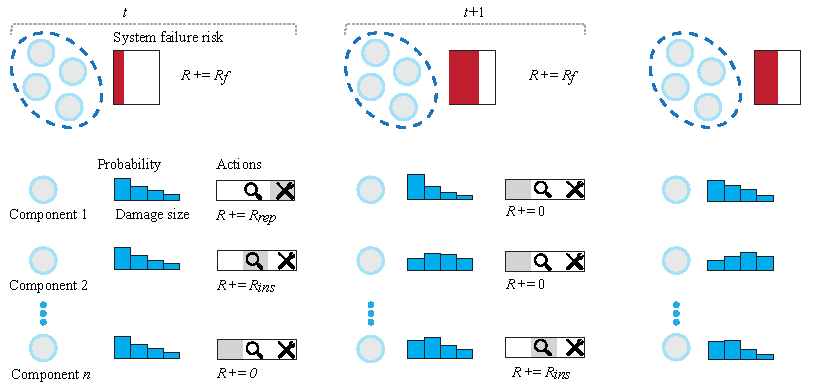
\includegraphics[width=\textwidth]{tex_thesis/figures/ch5/imp_intro.pdf}
\caption{Overarching representation of an infrastructure management problem.
The system failure risk is a function of the probability distribution over the components' damage condition. 
To control the system failure risk, components can be inspected or repaired at each time step $t$, and, typically, an agent controls one component.
The objective of IMP's problem is to maximise the expected sum of discounted rewards by balancing the system failure risk $R_f$ against inspections $R_{ins}$ and repairs $R_{rep}$, all three being negative rewards.
Here, we show three components with the same damage probability at time step $t$.
When a component is not inspected nor repaired, its damage probability evolves according to a deterioration process.
If a component is inspected, information from the inspection is also considered when updating the damage probability.
If a component is repaired, the damage probability resets to its initial damage distribution.}
\label{fig:ch5_imp_problem}
\end{figure}

IMP-MARL was introduced to generate more efficient strategies for managing engineering systems through cooperative MARL methods.
In IMP-MARL, each agent is responsible for managing one constituent component in a system, making decisions based on the damage probability of the component.
In addition to seeking to reduce component inspection and maintenance costs, agents should effectively cooperate to minimise the system failure risk.
To assess the capability of cooperative MARL methods for generating effective policies for IMP problems involving many components, state-of-the-art cooperative MARL methods are benchmarked in terms of scalability and optimality.
The benchmarked methods are presented in Chapter \ref{part:background} and Chapter \ref{ch:cooperation}.
Specifically, we benchmark five CTDE methods: QMIX, QVMix, QPLEX, COMA, and FACMAC, along with a decentralised method, i.e., IQL, and a centralised one, i.e., DQN.
All tested MARL methods are compared against expert-based heuristic policies, which can be categorised as a state-of-the-art method to deal with IMP problems in the reliability engineering community~\citep{LuqueDBN2019, morato2022optimal}.
In our study, three sets of IMP environments are investigated, including one related to offshore wind structural systems, where MARL methods are tested with up to 100 agents.
These environments can be set up with two distinct reward models, one incorporating explicit cooperative objectives.
Additionally, we ensure that the necessary code is publicly available so anyone can reproduce any published result\footnote{\url{https://github.com/moratodpg/imp_marl/}}.
This benefits an additional goal to facilitate the definition and implementation of new customisable environments.

From a societal perspective, more effective IMP policies contribute to a better allocation of resources.
Additional societal impact is also made by controlling the risk of system failure events.
For example, the failure of a wind turbine may affect the available electricity production. 
Beyond economic considerations, our proposed IMP-MARL framework can also be used to include sustainability and societal metrics within the objective function by accounting for those directly in the reward model.

Finally, the contributions of~\citep{leroy2023impmarl} presented in this chapter can be outlined as follows:
\begin{itemize}
  \item IMP-MARL is an open-source suite of environments, motivating the development of scalable MARL methods and the creation of new IMP environments, enabling the effective management of multi-component engineering systems and, as such, leading to a positive societal impact.
  \item In an extensive benchmark campaign, cooperative MARL methods are tested in high-dimensional IMP environments featuring up to 100 agents.
  The resulting management strategies are evaluated against expert-based heuristic policies.
  The source code is public so that we can reproduce our reported results and easily compare them with future developments.
  \item Based on the results, relevant insights for both machine learning and reliability engineering communities can be drawn, highlighting important challenges that must still be resolved.
  While cooperative MARL methods can learn superior strategies compared to expert-based heuristic policies, the relative performance benefit decreases in environments with over 50 agents.
  In specific environments, cooperative MARL policies are characterised by a high variance and sometimes underperform expert-based heuristic policies, suggesting the need for further research efforts.
\end{itemize}

\section{Related work} \label{sec:ch5_relatedwork}
As introduced, RL is not the single approach when solving IMP problems, and we hereafter discuss how MARL is becoming popular in the field.
Recent heuristic-based inspection and maintenance (I\&M) planning methods generate IMP policies based on an optimised set of predefined decision rules~\citep{LuqueDBN2019, Bismut2019OptimalDete}.
By evaluating only a set of decision rules out of the entire policy space, the previously mentioned approaches might yield suboptimal policies~\citep{morato2022optimal}.
In the literature, one can also find POMDP-based methods applied to the I\&M planning of engineering components, in most cases, relying on efficient point-based solvers~\citep{Papakonstantinou2014Part1, Papakonstantinou2014Part2, morato2022optimal}. 
When dealing with multi-component engineering systems, solving point-based POMDPs becomes computationally complex.
In that case, the policy and value function can be approximated by neural networks, enabling the treatment of high-dimensional engineering systems.
Value-based and policy-based methods have been proposed in the literature for the management of engineering systems~\citep{Andriotis2019ManagingLearning,andriotis2021deep,morato2022syst}, and some of them rely on CTDE methods~\citep{nguyen2022weighted, saifullah2022deep}.
Note that no open-source methods nor publicly available environments are provided in the abovementioned references.
This emphasises the importance of our efforts to enhance comparison and reproducibility within the reliability engineering community.

\section{IMP-MARL: A suite of Infrastructure Management Planning environments} \label{sec:ch5_imp}

In IMP, the damage condition of multiple components deteriorates stochastically over time, inducing a system failure risk that is penalised at each time step.
Components can be inspected or repaired to control the system failure risk, yet incurring additional costs.
The objective is to minimise the expected sum of discounted costs, including inspections, repairs, and system failure risk.
This can be achieved through the agents' cooperative behaviour, assigning component inspections and repairs while jointly controlling the system failure risk.
The introduced IMP decision-making problem can be modelled as a decentralised partially observable Markov decision process (Dec-POMDP).
We hereafter define the components of this Dec-POMDP and formally define the deterioration, inspection, transition and reward models in Section \ref{sec:ch5_models}.

\subsection{Environments formulation}
\label{sec:env_formulation}

\subsubsection{States and observations}
As introduced, each agent in IMP perceives $o^a_t$, an observation corresponding to its respective component damage probability and the current time step.
Each component damage probability transitions based on a deterioration model, defined in Section \ref{sec:ch5_models}.
The damage probability is also updated based on maintenance decisions.
Since the components' damage is not perfectly known, the state of the Dec-POMDP is defined as the collection of all components' damage probabilities along with the current time step: $s_t = (o_t^1, .., o_t^n, t)$.
Following the discussion in Chapter \ref{ch:cooperation}, IMP is a jointly observable Dec-POMDP.

\subsubsection{Actions and rewards}
Each agent controls a component and collaborates with other agents to minimise the system failure risk while minimising local costs associated with individual repair and/or inspection actions. 
At each time step $t$, an agent decides $u^a_t$ between (i) do-nothing, (ii) inspect, or (iii) repair actions.
Both inspection and repair actions incur significant costs, formally included in the Dec-POMDP framework as negative rewards, $R_{ins}$ and $R_{rep}$, respectively.
Moreover, the system failure risk is defined as $R_f= c_F \cdot p_{F_{sys}}$ where $p_{F_{sys}}$ is the system failure probability, and $c_F$ is the associated consequences of a failure event, encompassing economic, environmental, and societal losses.
In IMP, we include two reward models.
The first is a \emph{campaign cost} model where a global cost, $R_{camp}$, is incurred if at least one component is inspected or repaired, plus a surplus, $R_{ins}$ + $R_{rep}$, per inspected/repaired component.
This campaign cost explicitly incentivises agents to cooperate.
The second is a \emph{no campaign cost} model, where the campaign cost $R_{camp}=0$, and only component inspections and repairs costs are considered. 
Values of those costs are given in Section \ref{sec:ch5_rewardmodel}.
Acting on finite-horizon episodes that span over $T$ time steps, all agents aim at maximising the expected sum of discounted rewards
\begin{equation}
\label{eq:ch5_rewardimpmarl}
    \mathbb{E}[R_{0}] = \mathbb{E} \left[ \sum_{t=0}^{T-1} \gamma^t \left[ R_{t,f}+ \sum_{a=1}^n \left({R_{t,ins}^a} + {R_{t,rep}^a}\right)+R_{t,camp} \right] \right].
\end{equation}

\subsubsection{Real-world data}
While IMP policies are trained based on simulated data, the policies can then be deployed to applications where real-world data streams are available.
In that case, the damage condition of the components is updated based on collected real-world data, e.g., inspections.
 
\subsection{IMP-MARL environments}
\label{time stepsec:implement_env}

IMP-MARL provides three sets of environments to benchmark cooperative MARL methods.
For all three, components are exposed to fatigue deterioration during a finite-horizon episode, inducing the growth of a crack over $T$ time steps.
The first set of environments is \textit{k-out-of-n system} and refers to systems for which a system fails if (n-k+1) components fail.
Those systems have been widely studied in the reliability engineering community~\citep{barlow1984computing}. 
The second type of environment is \textit{correlated k-out-of-n system} and is a variation of the first one for which the initial components' damage distributions are correlated.
The last one is \textit{offshore wind farm} and allows the definition of environments for which a group of offshore wind turbines must be maintained.
They are graphically illustrated in Figure \ref{fig:env_categories}, and we hereafter provide details about these sets of environments.
The implementation details are provided in Appendix \ref{sec:ch5_appendix_imp_public_repo}.

\begin{figure}
\begin{subfigure}[t]{0.53\textwidth}
\centering
    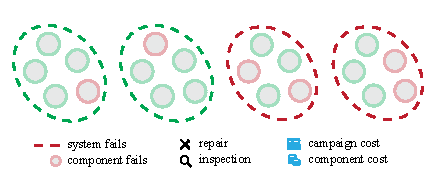
\includegraphics[width=1\linewidth]{tex_thesis/figures/ch5/fig2_mul/environments_v2_a.pdf}
    \caption{A k-out-of-n system environment.}
    \label{fig:env_categories_1}
\end{subfigure}%
\begin{subfigure}[t]{0.47\textwidth}
\centering
    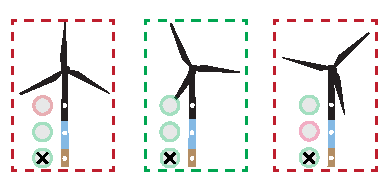
\includegraphics[width=1\linewidth]{tex_thesis/figures/ch5/fig2_mul/environments_v2_b.pdf}
    \caption{An offshore wind farm environment.}
    \label{fig:env_categories_2}
\end{subfigure}
%
\begin{subfigure}[t]{0.53\textwidth}
\centering
    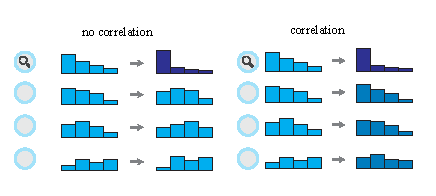
\includegraphics[width=1\linewidth]{tex_thesis/figures/ch5/fig2_mul/environments_v2_c.pdf}
    \caption{Uncorrelated and correlated initial damage distribution.}
    \label{fig:env_categories_3}
\end{subfigure}%
\begin{subfigure}[t]{0.47\textwidth}
\centering
    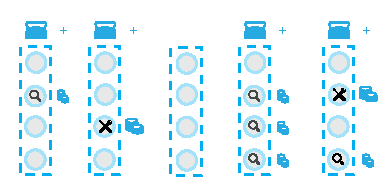
\includegraphics[width=1\linewidth]{tex_thesis/figures/ch5/fig2_mul/environments_v2_d.pdf}
    \caption{A campaign cost environment.}
    \label{fig:env_categories_4}
\end{subfigure}
\caption{
Visual representation of available IMP-MARL environment sets and options.
In \ref{fig:env_categories_1}, a 4-out-of-5 system fails if two or more components fail.
In \ref{fig:env_categories_2}, a wind turbine fails if any constituent component fails.
In \ref{fig:env_categories_3}, when the environment is under deterioration correlation, the information collected by inspecting one component also influences uninspected components.
In \ref{fig:env_categories_4} campaign cost environments, a global cost is incurred if any component is inspected and/or repaired, plus a surplus per inspected/repaired component. 
}
\label{fig:env_categories}
\end{figure}

\subsubsection{k-out-of-n system}
In this set of environments, the components' damage probability distribution, $p(d^a_t)$, is defined as a vector of 30 bins, each representing a crack size interval.
The failure probability of one component is defined as the probability indicated in the last bin.
The specificity of a k-out-of-n system is that it fails if (n-k+1) components fail, establishing a direct link between the system failure probability and the component failure probabilities.
The initial damage distribution among components is statistically independent for this first system, and the time horizon is $T=30$ time steps.
Since it is finite, we normalise each time step input and define $s_t = (p(d^1_t),..., p(d^n_t), t/T)$ and $o^a_t=(p(d^a_t), t/T)$.
The interest of this system is that, in many practical scenarios, the reliability of an engineering system can be modelled as a \textit{k-out-of-n system}.

\subsubsection{Correlated k-out-of-n system}
The second set of environments is the same as the previously defined one, with the difference that the initial damage distribution is correlated among all components.
Therefore, inspecting one component also provides information about other uninspected components, depending on the specified degree of correlation.
This setting is particularly challenging when approached in a decentralised mode without providing individual agents with component correlation information.
To address this issue, in addition to their 30-bin local damage probability, the agents perceive correlation information $\alpha_t$ common to all, updated based on inspection outcomes collected from all components.
We thus have: $s_t = (p(d^1_t),..., p(d^n_t),\alpha_t, t/T)$ and $o^a_t=(p(d^a_t), \alpha_t, t/T)$.
This damage correlation structure is inspired by practical engineering applications where initial defects among components are statistically correlated because components undergo similar manufacturing processes~\citep{morato2022optimal}.

\subsubsection{Offshore wind farm}
The third set of environments differs from previous ones as it considers a system with wind turbines.
Specifically, each wind turbine contains three representative components: (i) the top component located in the atmospheric zone, (ii) the middle component in the underwater zone, and (iii) the mudline component submerged under the seabed.
In this case, the mudline component is considered impossible to inspect or repair, as it is installed under the seabed in an inaccessible region.
Since only the top and middle components can be inspected or repaired, two agents are assigned for each wind turbine.
Furthermore, the damage probability, $p(d^a_t)$, is a vector with 60 bins and transitions differently depending on the component location in the wind turbine, as corrosion-induced effects accelerate deterioration in certain areas.
Besides individual component damage models, inspection techniques and their associated costs depend on the component location: inspecting or repairing the top components is cheaper than the middle one~\citep{giro2022inspection}.
Moreover, while the mudline component cannot be directly maintained, its damage probability also impacts the failure risk of a wind turbine.
In offshore wind farm environments, a wind turbine fails if one of its constituent components fails, and the overall system failure risk is defined as the sum of all individual wind turbine failure risks. In this case, $p(d^a_t)$ is modelled as a 60-bin vector, and the time horizon is $T=20$.
In this set of environments $s_t = (p(d^1_t),..., p(d^n_t), t/T)$ and $o^a_t=(p(d^a_t), t/T)$.

\section{Modelling infrastructure management in IMP-MARL}
\label{sec:ch5_models}
This section formally defines the deterioration, inspection, transition and reward models implemented in IMP-MARL.
These models drive the dynamics of the IMP-MARL environments.

\subsection{Deterioration models}
The deterioration processes introduced here correspond to fatigue deterioration mechanisms, yet corrosion, erosion, and many other practical infrastructure management problems can be similarly modelled.

\subsubsection{Correlated and uncorrelated k-out-of-n systems}
Throughout the following, the set of environments related to uncorrelated and correlated k-out-of-n systems are abbreviated as struct when referring to both. 
The structural components are exposed to fatigue deterioration in both k-out-of-n environments.
Unless a repair is undertaken, the crack size $d_t$ (i.e., damage condition) evolves over time $t$ following
\begin{equation} \label{Eq:ExamCrackGrow}
d_{t+1} =\bigg[ \Big(1-\frac{m}{2}\Big) C_{FM}S_{R}^m\pi ^{m/2}n_{S} + d_t^{1-m/2}\bigg] ^{2/(2-m)}   ,
\end{equation}
where $\ln(C_{FM}) \sim \mathcal{N} (\mu=-35.2, \sigma=0.5)$ and $m=3.5$ stand for material variables, which directly influence the crack growth~\citep{Ditlevsen2007StructuralMethods}.
Due to environmental and operational conditions, the components are subject to a dynamic load characterised by the stress range, $S_{R}  \sim  \mathcal{N} (\mu=70, \sigma=10$ N/mm$^2$), over $n_{S}=10^6$ annual stress cycles, i.e., the number of load cycles experienced by the structural component in one year.
At the initial step or after a component is repaired, the initial crack size is at its intact condition, defined by its initial distribution $d_0  \sim  \text{Exp} (\mu=1$ mm), and a component level failure occurs when the crack size exceeds a critical length of $d_c=20$ mm. 
The component failure probability $p_{F}$, defined as $p_{F}=P[g \leq 0]$, can be computed following a through-thickness failure criterion \cite{hlaing2022inspection}, where the failure limit at time step $t$ is formulated as $g_{t}=d_c-d_t$. At the system level, a failure event occurs if $n-k+1$ components fail, and its corresponding system failure probability, $p_{F_{sys}}$, can be efficiently computed as a function of all components failure probabilities, as proposed in~\citep{barlow1984computing}. 

The continuous crack size is discretised into discrete bins to enable efficient Bayesian inference when inspection indications are available.
Further details can be found in~\citep{morato2022optimal}. 
In a correlated k-out-of-n system, the initial crack size among components is correlated. 
In that case, the damage condition of each component is defined conditional on a common correlation factor, $\alpha$, via a Gaussian hierarchical structure~\citep{morato2022syst}.
In that case, the discretised damage bins should be defined conditionally based on the correlation factor.
Table \ref{Tab:discrExam} defines the specific discretisation implemented in our environments. 

\begin{table}
\begin{tabular}{llll}
\toprule
Environment & Variable & Interval boundaries & Bins\\
\midrule
struct & $d_t$ & $[0, \mathrm{exp}\{ \mathrm{ln}(10^{-4}):(\mathrm{ln}(d_{c})-\mathrm{ln}(10^{-4}))/28:\mathrm{ln}(d_{c})\},\infty ]$ & 30 \\
owf & $d_t$ & $[0, d_0:(d_c-d_0)/(60-2):d_c,\infty]$ & 60 \\
\bottomrule
\end{tabular}
\caption{Description of the discretisation scheme implemented.}
\label{Tab:discrExam}
\end{table}

\subsubsection{Offshore wind farm}
In this set of environments, abbreviated as owf in the following, a group of offshore wind substructures is considered, in which three representative structural components are modelled at different locations of the wind turbine: (i) at the atmospheric zone - upper level, (ii) at the splash zone - middle level, (iii) below the seabed - mudline. 
The deterioration, inspection, and cost models differ for each component. 
While the fatigue deterioration is calculated according to Equation \ref{Eq:ExamCrackGrow}, the expected dynamic load is defined based on industrial standards $S_r = q\Gamma(1+1/\lambda)Y$~\citep{dnv2015probabilistic},
corresponding to the expected value of a Weibull distribution defined by the scale parameters listed in Table \ref{tab:owf_fatigue}, $q \sim \mathcal{N}$, and shape factor, $\lambda=0.8$, weighted by a geometric parameter, $Y  \sim  \mathcal{LN} (\mu=0.1, \sigma=0.1)$. The initial crack size distribution is specified for all wind turbine components as $d_0  \sim  \text{Exp} (\mu=0.11)$ and the remaining specific fatigue variables associated with each wind turbine component are listed in Table \ref{tab:owf_fatigue}. 
At the wind turbine level, a failure event occurs if one component of the wind turbine fails. 
The wind turbine failure risk is thus defined as the probability of failure multiplied by the consequences of a failure event.
At the wind farm level, a wind turbine's damage condition does not influence the condition of the other wind turbines, and the wind farm system failure risk is defined as the sum of all turbines' failure risks.

\begin{table}
\centering
\begin{tabular}{lccc}
\toprule
 & Upper component & Middle component & Mudline component  \\
 \midrule
\multirow{2}{*}{$ln(C_{FM})$} & $\mu=-26.45$ & $\mu=-26.04$ & $\mu=-26.12$ \\
& $\sigma=0.12$ & $\sigma=0.4$ &  $\sigma=0.39$ \\
$m$ & 3 & 3 & 3 \\
\multirow{2}{*}{$q$}   & $\mu=10.21$  & $\mu=7.40$ & $\mu=6.74$  \\
 & $CoV=25\% $  & $CoV=25\% $ & $CoV=25\% $  \\
$d_c$ & 20 & 60 & 60 \\
$n_{S}$ & 5,049,216 & 5,049,216 & 5,049,216
\\
\bottomrule
\end{tabular}
\caption{Variables specified in the offshore wind farm deterioration models.}
\label{tab:owf_fatigue}
\end{table}

\subsection{Inspection models}
The inspection models implemented in IMP-MARL are hereafter described. 
They define the likelihood of retrieving a specific inspection outcome as a function of the damage size.

\subsubsection{Correlated and uncorrelated k-out-of-n systems}
The inspection model is normally characterised depending on the accuracy of the measurement instrument, formally specified through probability of detection (PoD) curves, in which the probability of observing a crack is defined as a function of the crack size~\citep{morato2022optimal}.
In this case, the inspection model is described by an exponential distribution $p({i_{d_t}}|d_t) \sim \text{Exp}(\mu = 8)$, defining the probability of observing a crack during an inspection.

\subsubsection{Offshore wind farm}
In this more practical set of environments, an eddy current inspection technique is considered, whose PoD is modelled by
\begin{equation} \label{eq:ex_pod1}
    p({i_{d_t}}|d_t) = 1 - \frac{1}{1+(d_t/\chi)^b}, 
\end{equation}
with $\chi=0.4$ and $b=1.43$ for the upper component and $\chi=1.16$ and $b=0.90$ for the middle component, according to industrial standards~\citep{dnv2015probabilistic}.
The middle component, located below the water level, can naturally expect less accurate inspection outcomes.

\subsection{Transition models}
An overview of the transition model is explained hereafter.
We refer the reader to~\citep{morato2022syst} for a more detailed description.
Since the crack size is discretised, the transition and inspection models can be stored in tables.
This allows our IMP-MARL environments to be efficiently simulated.
Alternatively, the crack size evolution could be directly computed at execution time, but this would incur an additional computational expense.

The transition model can be defined based on previously described deterioration and inspection models. 
If no inspection and maintenance are performed, i.e. do-nothing action, the damage condition progresses each time step according to the fatigue deterioration model formulated in Equation \ref{Eq:ExamCrackGrow}.
Note that a time step represents a year in our environments.
Considering that the damage follows a non-stationary deterioration process, the crack size distribution $d_{t+1}$ can be efficiently encoded as a function of the annual deterioration rate, $\tau_{t+1}$, and the crack size at the previous time step $d_{t}$ as $p(d_{t+1}|d_t,\tau_{t+1})$. 
Starting from $\tau_{0}=0$, the deterioration rate increases by one unit every year unless a component is repaired, in which case the deterioration rate returns to the initial value. 
The deterioration evolution over one time step is
\begin{equation} \label{eq:ex_pod2}
    p(d_{t+1}) =  \sum_{\tau_{t+1}} \sum_{d_t} p(d_{t+1}|d_t,\tau_{t+1}) p(d_{t}) p(\tau_{t+1}) .
\end{equation}
If an inspection action is planned, a damage indication $i_{d_{t+1}}$ is collected, and the crack size distribution can be updated via Bayes' rule
\begin{equation} \label{eq:ex_pod3}
    p(d_{t+1}|i_{d_{t+1}}) \propto  p(i_{d_{t+1}}|d_{t+1}) p(d_{t+1})   ,
\end{equation}
where the likelihood corresponds to the specific inspection model, described by a probability of detection curve, as mentioned before.
Since the damage probabilities are discrete, the normalisation constant can be straightforwardly computed by simply summing the unnormalised bins~\citep{morato2022optimal}.

To enable efficient computation of the deterioration evolution under correlation, a Gaussian hierarchical structure is adopted, in which the crack size probability $p(d_{t}|\alpha)$ is defined conditional on a common factor $\alpha$\citep{morato2022syst}. 
This work considers that the initial damage probabilities are equally correlated among components with a Pearson coefficient of 0.8. 
The damage transition, in this case, is
\begin{equation} \label{eq:ex_pod4}
    p(d_{t+1}|\alpha) =  \sum_{\tau_{t+1}} \sum_{d_t} p(d_{t+1}|d_t,\tau_{t+1}) p(d_{t}|\alpha) p(\tau_{t+1})   .
\end{equation}
Once an inspection outcome is available, the common correlation factor is updated based on the new information, thus influencing all components.
The likelihood of collecting one inspection indication given $\alpha$ is
\begin{equation}\label{Eq:margHyp}
p(i_{d_{t+1}}|\alpha)=\sum_{d_{t+1}} \Big[p(d_{t+1}|\alpha) p(i_{d_{t+1}}|d_{t+1})\Big]   ,
\end{equation}
and the correlation factor can then be updated
\begin{equation}\label{Eq:infHyp}
p(\alpha|i_{d_{t+1}}) \propto p(\alpha)p(i_{d_{t+1}}|\alpha) .
\end{equation}
Finally, the marginal damage probabilities are computed as:
\begin{equation}\label{Eq:margBel}
p(d_{t+1}) = \sum_{\alpha} \Big[p(d_{t+1}|\alpha)  p({\alpha}) \Big]   .
\end{equation}
 
\subsection{Reward model}\label{sec:ch5_rewardmodel}
The goal of the agents is to maximise the expected sum of discounted rewards, $\mathbb{E}[R_{0}] = \mathbb{E} \left[ \sum_{t=0}^{T-1} \gamma^t \left[ R_{t,f}+ \sum_{a=1}^n \left({R_{t,ins}^a} + {R_{t,rep}^a}\right)+R_{t,camp} \right] \right]$.
At each time step, the reward may include inspection $R_{ins}$ and repair $R_{rep}$ costs for all considered components, along with the system failure risk, which is defined as the system failure probability $p_{f_{sys}}$ multiplied by the associated consequences of a failure event $c_f$, formulated as $R_f = p_{f_{sys}} \cdot c_f$. A campaign cost $R_{camp}$ may also be included if that option is active.
The discount factor is defined as $\gamma=0.95$ in our experiments, and the specific rewards are listed in Table \ref{tab:rewards_det}.

\begin{table}
\centering
\begin{tabular}{llllll}
\toprule
Component & Campaign cost & $R_{ins}$ & $R_{rep}$ &  $c_f$ & $R_{camp}$ \\
\bottomrule
\multirow{2}{*}{struct} &  False & -1 & -20 & -10,000 & 0  \\ 
& True & -0.2 & -20 & -10,000 & -5   \\
\bottomrule
\multirow{2}{*}{owf upper level} & False & -1 & -10 & -1,000 & 0     \\
& True  & -0.2 & -10 & -1,000 & -5     \\
\multirow{2}{*}{owf middle level} & False & -4 & -30 & -1,000 & 0    \\
& True & -1 & -30 & -1,000 & -5    \\
\bottomrule
\end{tabular}
\caption{Rewards specified in our experiments.}
\label{tab:rewards_det}
\end{table}


\section{Experiments}\label{sec:ch5_experiments}
\subsection{Tested methods}
\label{sec:tested_method}
In an extensive benchmark campaign, we test seven RL methods.
The centralised controller, which has an action space that scales exponentially with the number of agents, is trained with the fully centralised method DQN and is the only method taking $s_t$ as input.
Furthermore, the fully decentralised method tested is IQL, in which all agents are independently trained.
Regarding the five CTDE methods, we investigate three value-based methods, QMIX, QVMix, and QPLEX, as well as two actor-critic methods, COMA and FACMAC.
We selected these methods for our benchmark study because they are well established, and their implementations are open-sourced and available within the PyMarl framework~\citep{samvelyan2019starcraft}.

All investigated RL methods are compared against a representative baseline in the reliability engineering community~\citep{LuqueDBN2019,morato2022syst}.
This baseline, referred to as expert-based heuristic policy, consists of a set of heuristic decision rules defined based on expert knowledge.
The heuristic policy includes both parametric and non-parametric rules.
Parametric decision rules depend on two parameters: (i) the inspection interval and (ii) the number of inspected components.
Non-parametric rules involve taking a repair action after detecting a crack and prioritising component inspections with higher failure probability.
To determine the best heuristic policy for each environment, all parametric rule combinations are evaluated over 500 policy realisations, thereby identifying the heuristic policy that maximises the expected sum of discounted rewards among all policies evaluated.

\subsection{Experimental setup}

The abovementioned seven MARL methods are tested in the three previously defined sets of IMP environments.
The environments differ by the number of agents and whether they include a campaign cost model.
The numbers of agents tested in the six types of environments are presented in Table~\ref{tab:experiments_details}.
To objectively interpret the variance associated with the examined MARL methods.
As explained in Section \ref{sec:ch5_imp}, an agent makes decisions based on its local damage probability, the current normalised time step, and sometimes correlation information is additionally provided, while the state, used by DQN and CTDE methods, encompasses all of the information combined.
In all cases, the action space features three possible discrete actions per agent, except for DQN, where the centralised controller selects an action among the $3^n$ possible combinations.
For complexity reasons, we only test DQN in k-out-of-n environments featuring 3 and 5 components and in environments with 1 and 2 wind turbines.

\begin{table}
\centering
\begin{tabular}{lccccc}
\toprule
IMP environments & \multicolumn{5}{l}{Number of agents}  \\
\midrule
k-out-of-n system & 3 & 5 & 10 & 50 & 100 \\
 Correlated k-out-of-n system & 3 & 5 & 10 & 50 & 100 \\
 Offshore wind farm & 2 & 4 & 10 & 50 & 100  \\
\bottomrule
\end{tabular}
\caption{Number of agents specified in all investigated IMP environments.}
\label{tab:experiments_details}
\end{table}

Given the importance of hyperparameters on the performance of RL methods~\citep{gorsane2022towards}, we initially selected their values reported by the original authors.
In an attempt to objectively compare the examined methods, parameters that play the same role across methods are equal.
Notably, the learning rate and gamma, among others, are identical in all experiments.
The controller agent network features the same architecture in all methods, consisting of a single GRU layer with a hidden state composed of 64 features encapsulated between fully connected layers and three outputs, one per action, except for DQN, where the network output includes $3^n$ actions.
In our case, DQN's architecture includes additional fully connected layers and a larger size of hidden GRU states.
Moreover, following common practice, agent networks are shared among agents, and thus, a single agent network is trained.
Specifically, we train only one network for all agents instead of training $n$ distinct agent networks.
The training process with a single agent network improves data efficiency because the same episode can be used to perform $n$ backpropagations through the same agent network, using $n$ different observations.
In contrast, if training is performed with $n$ different agent networks, only one backpropagation per agent network would be possible with a single episode.
To allow diversity in agents' behaviour, a one-hot encoded vector is also added to the input of this shared network to indicate which one of the $n$ agents is making the decision.
In CTDE methods, critics or mixers are also incorporated at the training stage with specific architectures according to each method and environment configuration.
In most cases, the neural networks are updated after each played episode based on 64 episodes sampled from the replay buffer containing the latest 2,000 episodes.
The only exception is COMA, which follows an on-policy approach, updating the network parameters every four episodes.
For value-based methods, the training episodes are played following an epsilon greedy policy, whereas test episodes are executed with a greedy policy.
The epsilon value is initially specified as 1 and linearly decreases to 0.05 after 5,000 time steps.
This is different for COMA and FACMAC. 
Appendix \ref{sec:ch5_appendix_param} and the source code list more details and all parameters.

The number of time steps allocated for one training realisation is 2 million time steps for all methods.
These 2 million training time steps are executed with training policies, e.g. $\epsilon$-greedy policy, saving the networks every 20,000 training time steps.
To evaluate them, we execute 10,000 test episodes and obtain the average sum of discounted rewards per episode per saved network.
These test episodes are executed with testing policies, e.g., the greedy policy.
We show in Appendix \ref{sec:ch5_appendix_variance} that 10,000 test episodes are needed due to the variance induced in the implemented environments.
We emphasise that ten training realisations are executed with different seeds for the same parameter values.
Finally, hardware and experiment duration are provided in Appendix \ref{sec:ch5_appendix_duration}.

\section{Results}\label{sec:ch5_results}

\begin{figure}
    \centering
    \includegraphics[width=\textwidth]{tex_thesis/figures/ch5/plot_explain_plot_gaussian.pdf}
    \caption{Visual description of the iterative process followed to generate the boxplots showcased in Figure \ref{fig:results}.
[Left] Learning curves corresponding to 10 QMIX training seeds in a k-out-of-n system with 50 agents. 
The markers highlight the policies that result in the highest expected sum of discounted rewards during evaluation, i.e., one policy per seed.
[Right] The ten selected policies are displayed at the top as a function of the expected sum of discounted rewards and the heuristic score obtained in this environment.
In the middle plot, we calculate and represent the ten selected policies as a function of normalised relative rewards, i.e., (x - h) / h.
Finally, a boxplot is constructed at the bottom based on the previously calculated ten normalised relative rewards, each representing a different seed.
}
\label{fig:explain_fig}
\end{figure}


\begin{figure}
    \centering
    \includegraphics[width=.87\textwidth]{tex_thesis/figures/ch5/boxplot_perc_limit.pdf}
\caption{Performance reached by MARL methods in terms of normalised discounted rewards with respect to expert-based heuristic policies in all IMP environments, H referring to the heuristics result.
Every boxplot gathers the best policies from each of 10 executed training realisations, indicating the 25th-75th percentile range, median, minimum, and maximum obtained results.
The coloured boxplots are grouped per method, vertically arranging environments with increasing $n$ agents, as indicated in the top-left legend boxes.
Note that the results are clipped at -100\%.
}
\label{fig:results}
\end{figure}

The benchmark campaign results are presented in a boxplot showcasing the relative performance of MARL methods with respect to expert-based heuristic policies in terms of their expected sum of discounted rewards.
Each boxplot represents each of the ten seeds by its best policy, which achieved the highest average sum of discounted rewards during evaluation.
The construction of such a boxplot is presented in Figure \ref{fig:explain_fig}, and all results are presented in Figure \ref{fig:results}.
Our analysis relies on relative performance metrics because the optimal policies are unavailable.
Finally, the corresponding learning curves and the best-performing policy realisations can be found in Appendix \ref{sec:ch5_appendix_add_results}.

\textbf{MARL-based strategies outperform expert-based heuristic policies.}
While heuristic policies provide reasonable IMP policies, most tested MARL methods yield a substantially higher expected sum of discounted rewards. 
Yet, the variance over identical MARL experiments is still sometimes significant.
In environments with no campaign cost, the performance achieved by MARL methods with respect to the baseline differs in configurations with a high number of agents, as shown at the top of Figure \ref{fig:results}.
In contrast, MARL methods reach better relative results in environments with many agents when the campaign cost model is adopted, as illustrated at the bottom of Figure \ref{fig:results}.
In general, the superiority of MARL methods with respect to expert-based heuristic policies is justified by the complexity of defining decision rules in high-dimensional multi-component engineering systems, where the sequence of optimal actions is challenging to predict based on engineering judgment~\citep{morato2022syst}.

\textbf{IMP challenges.}
In correlated k-out-of-n IMP environments, the variance over identical MARL experiments is higher than in the uncorrelated ones, emphasising a specific IMP challenge.
Under correlation, inspecting one component also provides information to uninspected components, impacting their damage probability and thus hindering cooperation between MARL agents.
Another challenge is imposed in offshore wind farm environments, where the benefits achieved by MARL methods with respect to the baseline are also reduced in environments with a high number of agents.
This can be explained by the fact that each wind turbine is controlled by two agents and is independent of other turbines in terms of rewards.
Each agent must then cooperate closely with only one of all agents, hence complicating global cooperation in environments featuring an increasing number of agents.

\textbf{Campaign cost environments.} Yet another challenge can be observed in campaign cost environments under 50 agents, where MARL methods' superior performance with respect to heuristic policies is more limited.
The aforementioned environments are challenging for MARL methods because agents should cooperate to group component inspection/repair actions together, saving global campaign costs.
In addition, the heuristic policies are designed to schedule group inspections, being favourable in this case automatically.
This is confirmed by the learning curves presented in Figures \ref{fig:learning_curves_cc_false} and \ref{fig:learning_curves_cc_true} in Appendix \ref{sec:ch5_appendix_add_results}.
On the other hand, in environments with more than 50 agents, MARL methods substantially outperform heuristic policies.
At least one component is inspected or repaired at each time step and the results reflect that avoiding global annual campaign costs becomes less crucial.

\textbf{Centralised RL methods do not scale with the number of agents.}
DQN reaches better results than heuristic policies, though it achieves lower rewards than CTDE methods in most environments despite benefiting from larger networks during execution.
This highlights the scalability limitations of such centralised methods, mainly because they select one action from each possible combination of component actions.

\textbf{IMP demands cooperation among agents.}
The results reveal that CTDE methods outperform IQL in all tested environments, especially those with many agents.
This confirms that realistic IMP problems demand coordination among component agents.
Providing only independent local feedback to each IQL agent during training leads to a lack of coordination in cooperative environments, also shown by \cite{Rashid2018}. 
However, the performance may be improved by enhancing networks' representation capabilities by including more neurons, yet this is true for all investigated methods.

\textbf{Infrastructure management planning via CTDE methods.}
Overall, CTDE methods generate more effective IMP policies than the other investigated methods, demonstrating their capabilities for supporting decisions in real-world engineering scenarios.
While Figure \ref{fig:results} presents the variance of the best results across runs, the learning curves further confirm this finding in Appendix \ref{sec:ch5_appendix_add_results}.
In particular, QMIX and QVMIX generally learn effective policies with low variability over runs. 
Slightly more unstable, QPLEX also yields results similar to those of QMIX and QVMIX in terms of achieved results.
While being able to outperform heuristic policies in almost every environment, FACMAC exhibits a high variance among runs.
However, FACMAC effectively scales up with the number of agents and environment complexity (as reported by their authors \citep{peng2021facmac}), achieving some of the best results in IMP environments with over 50 agents as well as in correlated IMP environments.
The results also suggest that COMA is our benchmark's least scalable MARL method.
This can be attributed to the fact that the computation of the critic's counterfactual becomes challenging with an increasing number of agents.
Additional results are presented in Appendix \ref{sec:ch5_appendix_add_results}, where many tables and figures can be found.

\section{Discussion and future work}\label{sec:ch5_discusconclu}
%\section{Conclusions} \label{sec:conclusions}
This work offers an open-source suite of environments for testing the scalability of cooperative MARL methods for efficiently generating IMP policies.
Through our publicly available code repository, we also encourage the implementation of additional IMP environments, such as bridges, transportation networks, pipelines, and other relevant engineering systems.
This allows specific disciplinary challenges to be identified in a common simulation framework.
Based on the reported benchmark results, we can conclude that CTDE methods generate effective infrastructure management policies in real-world engineering scenarios.
While the results reveal that MARL methods outperform expert-based heuristic policies, additional research efforts should still be devoted to developing scalable cooperative MARL methods.

While we model the IMP decision-making problem as a Dec-POMDP, modelling IMP problems as mean-field games~\citep{lauriere2022learning} is a promising direction to be considered in environments with an increasing number of agents.
Moreover, specific improvements are still required in environments where a global cost is triggered from the actions taken by any local agent, e.g., global campaign cost.
Besides, more stable training is still needed in environments where local information perceived by one agent can influence the damage condition probabilities of others, as in the correlated IMP environments.
More realistic and challenging environments for cooperative MARL methods could be investigated.
One example is assigning campaign costs to specific groups of components instead of specifying only one global campaign cost.
Another example is to address systems composed of more heterogeneous components.\cleardoublepage
\part{Cooperate against an opposing team}\label{part:compet}
\chapter{Competition}\label{ch:competition}
\begin{chapter_outline}
Outline
\end{chapter_outline}

\damien{Deadline: 20/02}
\section{Introduction}

nash vs pareto

\section{1 vs 1 competition}
\section{General sum game}\cleardoublepage
\chapter{Symmetric two team Markov game}\label{ch:2teams}
\begin{chapter_outline}
Outline \citep{leroy2022twoteam}
\end{chapter_outline}

\section{Introduction}


In this paper, we identify the best learning scenario to train a team of agents to compete against multiple possible strategies of opposing teams.
We evaluate cooperative value-based methods in a mixed cooperative-competitive environment.
We restrict ourselves to the case of a symmetric, partially observable, two-team Markov game.
We selected three training methods based on the centralised training and decentralised execution (CTDE) paradigm: QMIX, MAVEN and QVMix.
For each method, we considered three learning scenarios differentiated by the variety of team policies encountered during training.
For our experiments, we modified the StarCraft Multi-Agent Challenge environment to create competitive environments where both teams could learn and compete simultaneously.
Our results suggest that training against multiple evolving strategies achieves the best results when, for scoring their performances, teams are faced with several strategies.
%This conclusion whether the stationary strategy is better than all trained teams or not.
%While this result is well known, the main contribution is its demonstration in new environments with these algorithms.


Many applications exist where two teams of multiple agents compete, such as in games (Pommerman \citep{resnick2018pommerman}) or in robotics (RoboCup \citep{kitano1997robocup}).
In certain use-cases, agents are not fully aware of the entire environment, such as in Cyber Physical Production Systems \citep{phan2020learning}, Hide and Seek \citep{baker2019emergent} or Capture the Flag \citep{jaderberg2019human}.
To solve the challenges faced within all these applications, reinforcement learning (RL) is a solution.
RL is a paradigm of machine learning where an agent interacts with an environment by selecting actions based on its observations and receives rewards \citep{sutton2018reinforcement}.
Multi-agent RL (MARL) is an extension of single-agent RL (SARL) where a single agent acts in the environment.
The value-based method is a family of RL methods where an agent learns the highest sum of rewards (value) it can achieve by selecting a given action at a given state.
We distinguish different MARL settings based on the goals of agents. 
They can share the same goal and cooperate, or compete for an opposite goal to the detriment of other agents.
In this paper, we evaluate value-based methods designed for cooperative settings to train agents in a partially observable mixed cooperative-competitive environment where two teams of cooperative agents compete to achieve an opposing goal. Our objective is to identify how to train a team to be resilient to different adversarial strategies.

The cooperative setting can be considered as a decentralised partially observable Markov decision process (Dec-POMDP) \citep{DecPomdp}, which is a framework where agents have partial observations and share the same rewards.
An example is the StarCraft Multi-Agent Challenge (SMAC) \citep{samvelyan2019starcraft}.
The partial observability of agents implies that the control is prevented from being centralised.
This means that it is not possible to control all agents of a team as if they were a single agent.
Therefore, decentralisation is required and each agent must select actions independently based on its own observations.
A first solution is to train each agent of the team independently using SARL methods.
Another possibility is the centralised training with decentralised execution (CTDE), where information about all agents is exploited during training but not during execution.
CTDE methods have shown better results than independent methods in Dec-POMDP.
In this paper, we selected three CTDE value-based methods QMIX \citep{Rashid2018}, MAVEN \citep{Mahajan2019MAVEN:Exploration} and QVMix \citep{leroy2020qvmix}. Other existing methods are discussed in Section \ref{sec:related}.

RL has not been the first choice to solve complex competitive two-player games.
For example, we think of Deep Blue \citep{campbell2002deep}.
However, the improvements in hardware has made possible to apply RL algorithms to play such games with partial observability \citep{silver2018general} or even games with more than two competing agents, such as Quake III Arena in Capture the Flag mode \citep{jaderberg2019human} or StarCraft \citep{vinyals2019grandmaster}.
To train such agents to compete, a paradigm called self-play is used.
Agents play against themselves, allowing them to face evolving strategies and to improve their skills.
In more complex games, a population of learning agents is created by duplicating some of the agents during training to enforce the diversity of opponents.
This allows agents to improve their skills while remaining competent against previously encountered strategies.
In most of the mixed cooperative-competition papers mentioned before, agents are trained with independent SARL methods in self-play or within a population, except for Baker et. al. \cite{baker2019emergent} who chose a CTDE method that exploit the state of the environment during training.

In this paper, we mix cooperative and competitive methods to train teams to compete in a symmetric two-team Markov game where two teams composed of the same agents compete.
Specifically, we study the difference between three learning scenarios: learning against a stationary team policy, against a single evolving team strategy (self-play), and against multiple evolving team strategies within a population of learning teams.
To perform these experiments and to study the performances of each learning scenario, we created a new competitive environment by modifying SMAC which has been designed for cooperation.
We chose symmetrical competition to ensure fair and balanced competition in addition to the possibility of controlling either team with the same agents. 
In two different SMAC environments, we trained teams with three value-based CTDE methods, QMIX, MAVEN and QVMix, each with the three learning scenarios and we then analysed how they perform when faced with multiple opposing strategies.
Our results suggest that when competing with several possible strategies, teams trained in a population achieve the best performance, but a selection process is required to select the best team.
We reached this conclusion irrespective of whether or not the stationary strategy was better than all trained teams.

We define the two-team Markov game and CTDE value-based methods in Section \ref{sec:background}.
The competitive SMAC is described in Section \ref{sec:SMAC}.
In Section \ref{sec:Learning}, we detail the learning scenarios and the performances criteria.
Details of the experiments are provided in Section \ref{sec:experiments} and their results in Section \ref{sec:results}.
The related work is presented in Section \ref{sec:related} followed by the conclusion in Section \ref{sec:conclusion}.

\section{Two-team Markov game}
%\subsection{Symmetric two-team Markov game}
Our framework is a special case of a Markov game \citep{MarkovGames}.
Specifically, we are in a symmetric, mixed cooperative-competitive, partially observable two-team Markov game defined by a tuple $[\mathcal{S}, O, \mathcal{Z}, \mathcal{U}, n, R, P, \gamma]$, where two teams of $n$ agents each compete by choosing an action at every timestep $t$.
Let $\mathcal{I}=\{1,..,n\}$ and $\mathcal{J}=\{1,-1\}$, the $i^{th}$ agent of the $j^{th}$ team is denoted by $a_{i, j} (i \in \mathcal{I}, j \in \mathcal{J})$ when it is not shortened to $a$.
Its action space is defined by $\mathcal{U}_{a_{i, j}}$.
Since we assume team symmetry, agents $a_{i, 1}$ and $a_{i, -1}$ share the same action space ($\forall i$).
The joint set of $n$ action spaces is denoted by $\mathcal{U}=\bigtimes_{i\in \mathcal{I}} \mathcal{U}_{{a_{i, 1}}} = \bigtimes_{i\in \mathcal{I}} 
\mathcal{U}_{{a_{i, -1}}}$.
The state of the environment at timestep $t$ is $s_t \in \mathcal{S}$ where $\mathcal{S}$ is the set of states, and $o_t^{a} \in \mathcal{Z}$ is the observation of this state perceived by the agent $a$, where $\mathcal{Z}$ is the set of observations. The observation function $O: \mathcal{S} \times I \times J \rightarrow \mathcal{Z}$ determines $o_t^a$.
At each timestep $t$, each agent simultaneously executes an action $u_t^{a} \in \mathcal{U}_a$ such that the state $s_t$ transits to a new state $s_{t+1}$ with a probability defined by the transition function $P(s_{t+1}|s_t, \mathbf{u_t}): \mathcal{S}^2 \times \mathcal{U}^2 \rightarrow \mathbb{R^+}$ where the joint action $\mathbf{u_t} = \{\mathbf{u^1_t}, \mathbf{u^{-1}_t}\} = \bigcup_{i \in \mathcal{I}, j \in \mathcal{J}} u_t^{a_{i, j}}$. 
After the joint action is executed, common team rewards $\{r_t^1, r_t^{-1}\} = R(s_{t+1}, s_t, \mathbf{u_t}): \mathcal{S}^2 \times \mathcal{U}^2 \rightarrow \mathbb{R}^2$ are assigned to agents.
An agent $a$ chooses its action based on its current observation $o_t^{a} \in \mathcal{Z}$ and its history $\tau_t^{a} \in (\mathcal{Z} \times \mathcal{U}_a)^{t-1}$.
Its policy is the function $\pi^{a}(u_t^{a}|\tau_t^{a},o_t^{a}): (\mathcal{Z} \times \mathcal{U}_a)^t \rightarrow \mathbb{R^+}$ that maps, from its history and the current observation, the probability of taking action $u_t^{a}$.
The team policy is denoted by $\mathbf{\pi_j}=\bigcup_{i \in \mathcal{I}} \pi^{a_{i, j}}$.

During an episode, the cumulative discounted reward obtained from timestep $t$ over the next $T$ timesteps by team $j$ is defined by $R_{t}^j = \sum_{k=0}^{T-1} \gamma^k r^j_{t+k}$ where $\gamma \in [0, 1)$ is the discount factor.
The goal of each agent is to find the optimal team policy that maximises the expected cumulative discounted reward: $\mathbf{\pi_j^{*}} =\argmax_{\mathbf{\pi_j}} \mathbb{E}[R^j_0|\mathbf{\pi_{j}}, \mathbf{\pi_{-j}}]$ that depends on the other team policy $ \mathbf{\pi_{-j}}$.
To compute the optimal policy, in value-based methods, we rely on the value function $V^{\mathbf{\pi}, j}(s)=\mathbb{E}[R^j_t | s_t = s, \mathbf{\pi}]$, called the $V$ function.
We also define the state-joint-action value function $Q^{\mathbf{\pi}, j}(s,\mathbf{u})=\mathbb{E}[R^j_t | s_t=s, \mathbf{u^j_t}=\mathbf{u}, \mathbf{\pi}]$, called the $Q$ function.
The corresponding individual state-action value function of an agent policy is defined by $Q^{\mathbf{\pi}, a_{i, j}}(s,u)=\mathbb{E}[R^j_t | s_t=s, u^{a_{i, j}}_t=u, \mathbf{\pi}]$ and denoted as $Q_a$ for the sake of conciseness. Since agents share the same reward in the same team, $Q^{\mathbf{\pi}, a_{i, j}}(s,u)=Q^{\mathbf{\pi}, j}(s,\mathbf{u})$.
Note that the symmetry allows one to control both teams with the same policy.

It is possible to obtain the Dec-POMDP \citep{DecPomdp} definition from that of the two-team Markov game by constraining one team to have a stationary policy.
The other team would then be the only team learning and the two-team Markov game can be considered as a Dec-POMDP.
Its formal definition is easily derived from that of the two-team Markov game by eliminating team considerations and ignoring the $j$.
In our experiments, teams are trained with value-based methods designed for Dec-POMDP.
As stated in the introduction, it is not possible to learn only the state-joint-action value function $Q(s,\mathbf{u})$ to centrally control the agents because agents must select their action based only on $(o, \tau)$ and do not perceive $s$.
A solution is known as independent Q learning (IQL) \citep{Tan1993} and consists in training agents to learn $Q_a$ independently, ignoring the presence of other learning agents.
Another solution is to exploit more information during training but only the available $(o, \tau)$ during execution.
It is a paradigm called centralised training with decentralised execution (CTDE).
The algorithms tested in this paper, QMIX \citep{Rashid2018}, MAVEN \citep{Mahajan2019MAVEN:Exploration} and QVMix \citep{leroy2020qvmix} exploit this paradigm.
All three methods learn $Q(s_t,\mathbf{u_t})$ as a factorisation of $s_t$ and $Q_a$ $\forall a$ during training.
The $Q_a$ are no longer $Q$ functions but are utility functions used to select actions which are retained for the execution.
There exists a condition to factorise $Q(s_t,\mathbf{u_t})$, called the Individual-Global-Max condition (IGM), that requires that $\argmax_{\mathbf{u_t}} Q(s_t, \mathbf{u_t}) =\bigcup_{a}\argmax_{u_t^{a}} Q_{a}$ \citep{Son2019QTRAN:Learning}.
In QMIX, $Q_a$ factorise $Q(s_t,\mathbf{u_t})$ with a hypernetwork.
The weights of each $Q_a$ in the factorisation are computed based on $s_t$ and are constrained to be positive to ensure IGM.
MAVEN follows the same principle of QMIX with an additional hierarchical policy network that modifies each $Q_a$ in order to influence agents' behaviour and to improve their exploration capacity.
QVMix is an extension of the Deep Quality-Value (DQV) family of algorithms \citep{sabatelli2018deepQV,sabatelli2020deep} applied to QMIX where agents learn both the $Q$ and the $V$ functions.
Those value-based methods which were initially developed for solving Dec-POMDP are thoroughly detailed in Appendix \ref{app:vbmethod}.
We chose QMIX because of its popularity, MAVEN because of its exploration technique which outperforms QMIX in complex scenarios, and QVMix because it has proven to be competitive with these previously mentioned algorithms.
Other methods have been developed as described in Section \ref{sec:related}.

\section{Competitive StarCraft Multi-agent challenge}
\label{sec:SMAC}

To perform our experiments, we created a new environment by modifying the StarCraft Multi-Agent Challenge (SMAC) \citep{samvelyan2019starcraft} to create a competitive environment. 
SMAC has been developed to train a team to cooperate in a competitive environment but only against the built-in StarCraft AI which has a stationary strategy. 
We adapted\footnote{\label{foot_note_code}\url{github.com/PaLeroy/competSmac} - \url{github.com/PaLeroy/competPymarl}} both SMAC and the associated learning framework PyMARL \citep{samvelyan2019starcraft}.
It is now possible to control both opposing teams in SMAC, as well as train them simultaneously.
In competitive SMAC, the goal remains unchanged, and it is to defeat the opposing team, by inflicting sufficient damage to reduce the hit points of all opponents to zero.
The winning team is the one that ends up with the highest sum of remaining hit points at the end.
If both teams end up with the same total of hit points, it is a draw.
In SMAC, a map is the name given to the different scenarios, and from an RL perspective, a different map is a different environment.
For our experiments, we have chosen the $3m$ and $3s5z$ maps.
In the $3m$ map, two teams of three marines compete for a maximum $100$ timesteps.
In the $3s5z$ map, two teams of three stalkers and five zealots compete for a maximum $150$ timesteps.
More details about these two maps and competitive SMAC can be found in Appendix \ref{app:smac}.


its relative position with respect to the centre of the map 


\section{Learning scenarios and performances criteria}
Our goal is to train a team to be resilient to different adversarial strategies.
We test three different learning scenarios differentiated by the diversity of opponents' strategies encountered during training.
Thanks to the environment symmetry, the trained teams can act as any of the two teams in our environments.
In the first learning scenario, the team is trained against a stationary strategy, which we refer to as a heuristic.
As introduced in Section \ref{sec:background}, such configuration is a Dec-POMDP, framework for which CTDE methods are designed.
The second scenario is called self-play where the team is trained by playing against itself and thus facing a strategy that continuously improves at the same learning speed.
This scenario has proven its value in competitive MARL \citep{baker2019emergent}.
In the third scenario, a population composed of several teams is trained with the same method.
Teams either play against themselves or against other learning teams.
Self-play is the special case of a training population composed of a single team.
This learning scenario has proven itself when the number of winning strategies is large, such as in StarCraft \citep{vinyals2019grandmaster}.
The latter trained a growing population of agents but in this paper, the size of the training population is fixed to five to reduce computational complexity.

After training, we evaluate teams with the Elo rating system \citep{elo1978rating}.
Its purpose is to assign each player of a population with a rating.
From these ratings, one can compute the probability that a player will win when facing another one.
Individuals' scores are updated based on the outcome of the episode  and their current Elo scores.
The Elo rating system is formally described in Appendix \ref{app:elo}.

We form test populations to compute Elo scores in different configurations.
To evaluate only the learning scenarios, we form one test population for each CTDE method with teams trained with all learning scenarios.
To evaluate the performances of the heuristic, we add it in the previously defined test populations to form new ones.
To find the best learning scenario/training method pair, we group all trained teams in two test populations, with and without the heuristic.
To evaluate training efficiency and heuristic performances, each trained team is tested along with training against the heuristic and against teams trained with other learning scenarios but using the same CTDE method.

\section{Elo score}
\label{app:elo}
The purpose of the Elo rating system \citep{elo1978rating} is to assign each player of a population with a rating $R$ to rank them.
From these ratings, one can compute the probability that a player will win when facing another one.
Let $R_A$ and $R_B$ be the ELO scores of player A and B, respectively.
In such a context, the probability that player A (B) wins over player is B (A) is computed using Equation \ref{eq:elo_predict1} (\ref{eq:elo_predict2}) given below.

\begin{align}
    \label{eq:elo_predict1}
    E_A=\frac{10^{R_A/400}}{10^{R_A/400} + 10^{R_B/400}}
    \\
    \label{eq:elo_predict2}
    E_B=\frac{10^{R_B/400}}{10^{R_A/400} + 10^{R_B/400}}
\end{align}%

One can see that $E_A + E_B = 1$.
The number $400$ can be considered as a parameter.
It determines that if the Elo score of player A is 400 points above that of B, it has a ten-times greater chance of defeating B.
In order to update the rating of player $A$ after a game, we take into account its score $S_A$ which is equal to $1$ for a win, $0$ for a loss and $0.5$ for a draw.
The updated score $R'_A$ is defined in Equation \ref{eq:elo_update} where $cst$ is a constant that defines the maximum possible update of the Elo score.
Typically, $cst$ is $32$ but for our experiments, we set it to $10$ to decrease the amplitude of oscillations in the Elo score during tests.

\begin{equation}
    \label{eq:elo_update}
    R'_A = R_A + cst * (S_A - E_A)
\end{equation}



\section{Experiments}

For our experiments, teams were trained with three learning scenarios (Sec. \ref{sec:Learning}) and with three CTDE methods, QMIX, MAVEN and QVMix (Sec. \ref{sec:background}), in two different environments (Sec. \ref{sec:SMAC}).
We conducted the same experimental process for both environments.
For each method, each learning scenario was executed ten times and stopped after each team had exploited $10^7$ samples.
For each method, this resulted in ten teams trained against the heuristic requiring $10^7$ environment timesteps, ten teams trained in self-play requiring $5\times10^6$ environment timesteps and ten training populations of five teams leading to $50$ teams trained within populations requiring at least $5\times10^7$ environment timesteps.
Therefore, in total, $210$ teams of nine types were trained in both environments.

To train teams against the heuristic, it was ensured that they play the same number of episodes as team $j=1$ and team $j=-1$.
Concerning the training within a population, each team had an equal chance of playing as team $j=1$ or team $j=-1$, meaning an equal chance to play against any team in the population, including itself.
For all learning scenarios and methods, network architectures and parameters are the same to ensure fair comparison.
Learning parameters were determined by default configurations provided by their different authors \citep{Rashid2018,Mahajan2019MAVEN:Exploration,leroy2020qvmix}.
More details about the training parameters is provided in Appendix \ref{app:train_param}.
The main differences with the original are that the epsilon anneal time is set to $2$ million instead of $0.5$ million and that the networks are updated every eight episodes in $3m$ and every episode in $3s5z$.
As in the literature, individual networks of each team share the same parameters to improve learning speed. We present training times in Appendix \ref{app:train_time}.

In this paper, the heuristic is based on two rules.
It moves toward the starting point of the opponent's team until it reaches the opposite side of the map and stops.
If there are enemies within its shooting range, it attacks the nearest one.
This heuristic is slightly different from StarCraft's built-in AI originally used to train teams to cooperate in SMAC.
The built-in AI also moves toward the other side but selects targets based on a priority score.
It will choose to attack the closest unit with the highest priority and this unit will remain the target until its priority drops or it can no longer be attacked.
A unit's priority score is based on its type and current action.
For example, if two of the same units attack and the targeted unit stops attacking, its priority score will drop and the built-in AI will select the other unit to attack.
This is the main difference with our heuristic which will attack the nearest unit regardless of its action and its priority.
Results show that our heuristic is harder to beat than the one provided in SMAC.
Finally, while both maps are denoted as easy in \citep{samvelyan2019starcraft}, the task of learning everything from scratch is not.
When learning against the heuristic, teams do not need to learn how to find their opponents, because they automatically move towards them.
When they learn in self-play or within a population, they first need to learn where to find opponents before they learn to face them.
This increase in learning complexity compared to their cooperative version led us to this choice of maps, motivated by a compromise between computational complexity and learning complexity.

As described in Section \ref{sec:Learning}, we form test populations to evaluate teams with the Elo rating system.
For both environments, we have three test populations of 70 teams trained with the same method and the three learning scenarios.
We also have one test population with all the 210 trained teams.
We created four additional test populations from the four previously defined by adding the heuristic to them.
In practice, to compute the Elo scores in these 16 test populations, each team plays $20$ games against all the other teams in a randomised order.
Every team starts with an Elo score of $1000$ and we set the maximum Elo score update to $10$, which is sufficiently small for our population sizes.
In Section \ref{sec:results}, we analyse the distribution of Elo scores after every team had finished its testing games.

During training, team neural network parameters are recorded every $2\times10^5$ timesteps until the $10$ millionth played timestep.
The test populations are composed of the agents whose network parameters correspond to those recorded at the 10 millionth timestep.
The other saved networks allow one to evaluate teams' performances during training.
We evaluate teams trained with a method and a learning scenario against the heuristic and against all teams trained with the same method but a different learning scenario.
We analysed the win rates along training timesteps of these different matchups when teams play $24$ games against each other.
For example, and for the same method, each ten teams trained in self-play played $24$ games against all the $50$ teams trained within a population and against the $10$ teams trained against the heuristic.

\section{Results}

We present the Elo scores of teams with box plots in Figure \ref{fig:elo_method} when the test population contains teams trained with the same method.
We first focus on performances when the heuristic is not in the test population (Fig. \ref{subfig:elo_no_h_3m}, \ref{subfig:elo_no_h_3s5z}).
The first observation is that the best teams are the ones trained within a population, except with MAVEN in $3s5z$ (Fig. \ref{subfig:3s5z_elo_no_h_methodMAVEN}) for which the differences between learning scenarios are smaller.
We discuss these differences later.
The second observation is that the population scenario has the highest variance.
To understand this, we also plot the box plots corresponding to the ten teams that achieved the highest Elo score of each training population, denoted by \textbf{BP}.
These box plots confirm that there is a difference between teams of the same training population and a selection must be performed to find the best one, so as to optimise the performances of this learning scenario.
Training against the heuristic is the worst scenario, arguably because agents do not generalise to other strategy than the heuristic.
However, the heuristic is not in these test populations and its impact is the concern of later analysis.
The performances of teams trained in self-play lies in between the two other learning scenarios.
While some teams achieve Elo scores close to the best teams of each training population, the scores of others are lower than the lowest scores of teams trained within population.

\begin{figure*}[h]
\captionsetup[subfigure]{justification=centering}
    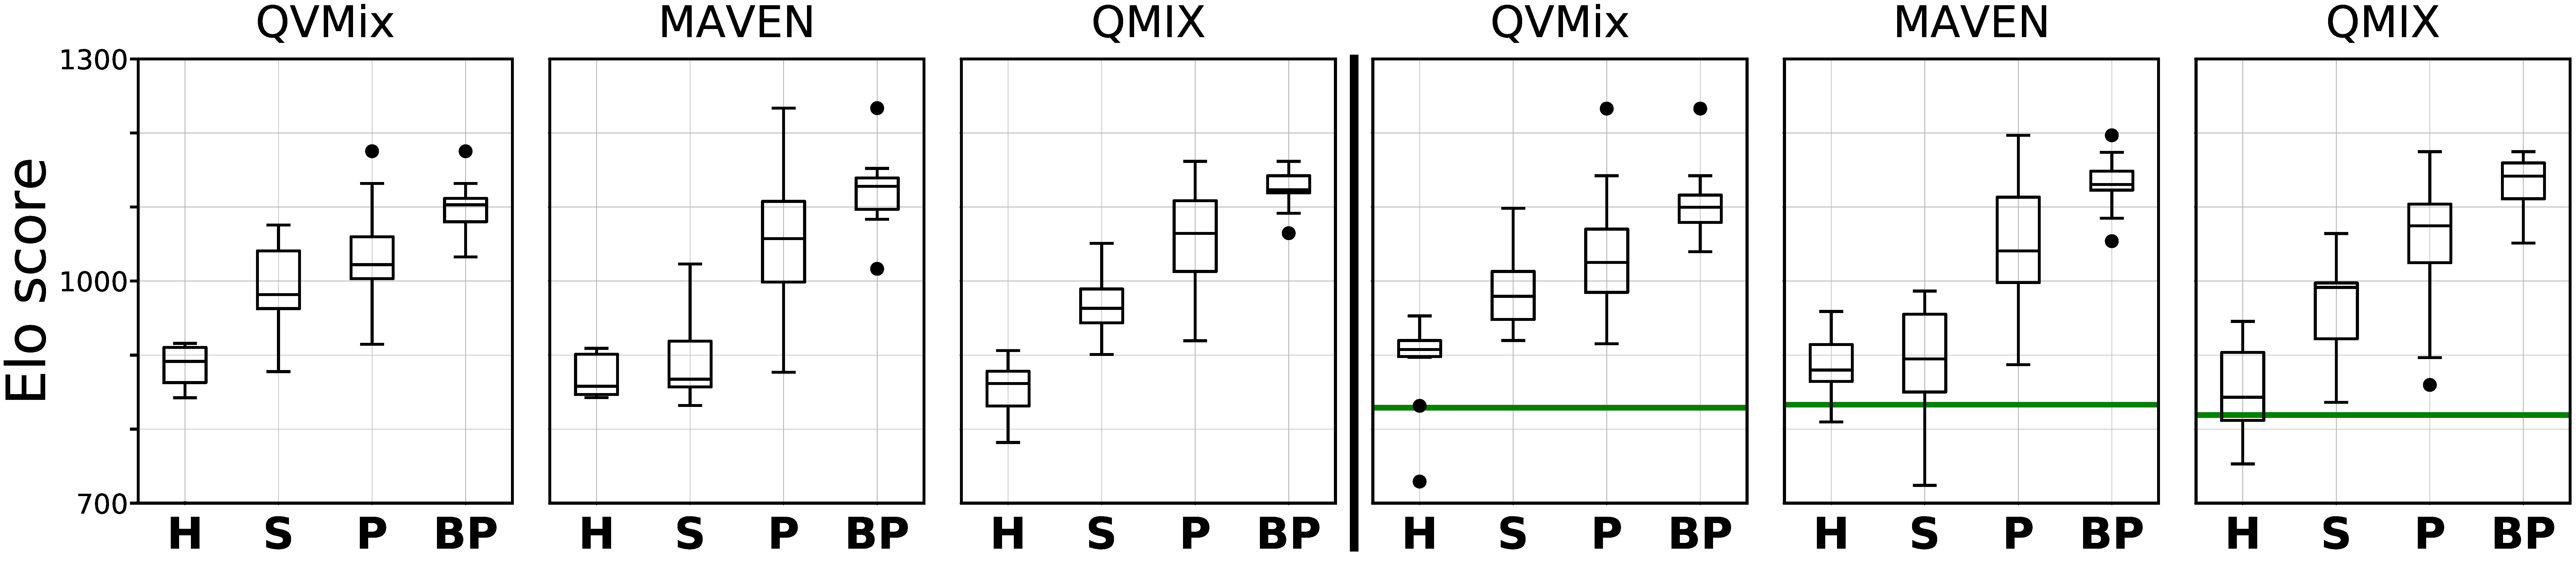
\includegraphics[width=\textwidth]{tex_thesis/figures/ch7/3m_tiny_six_qvmix_maven_qmix.pdf}
    \begin{subfigure}{.045\textwidth}
    \centering
    \caption*{}
    \end{subfigure}%
    \begin{subfigure}{.455\textwidth}
        \begin{subfigure}{.33\textwidth}
            \renewcommand\thesubfigure{\alph{subfigure}.1}
          \centering
          \caption{}
          \label{subfig:elo_no_h_methodQVMIX}
        \end{subfigure}%
        \begin{subfigure}{.33\textwidth}
        \addtocounter{subfigure}{-1}
            \renewcommand\thesubfigure{\alph{subfigure}.2}
          \centering
          \caption{}
          \label{subfig:elo_no_h_methodMAVEN}
        \end{subfigure}%
        \begin{subfigure}{.33\textwidth}
        \addtocounter{subfigure}{-1}
            \renewcommand\thesubfigure{\alph{subfigure}.3}
          \centering
          \caption{}
          \label{subfig:elo_no_h_methodQMIX}
        \end{subfigure}%
    \centering
    \addtocounter{subfigure}{-1}
    \caption{$3m$ map \textbf{without} heuristic.}
    \label{subfig:elo_no_h_3m}
    \end{subfigure}%
    \begin{subfigure}{.455\textwidth}
        \begin{subfigure}{.33\textwidth}
        \renewcommand\thesubfigure{\alph{subfigure}.1}
          \centering
          \caption{ }
          \label{subfig:elo_h_methodQVMIX}
        \end{subfigure}%
        \begin{subfigure}{.33\textwidth}
         \addtocounter{subfigure}{-1}
        \renewcommand\thesubfigure{\alph{subfigure}.2}
          \centering
          \caption{ }
          \label{subfig:elo_h_methodMAVEN}
        \end{subfigure}%
        \begin{subfigure}{.33\textwidth}
            \addtocounter{subfigure}{-1}
            \renewcommand\thesubfigure{\alph{subfigure}.3}
          \centering
          \caption{ }
          \label{subfig:elo_h_methodQMIX}
        \end{subfigure}%
    \centering
    \addtocounter{subfigure}{-1}
    \caption{$3m$ map \textbf{with} heuristic.}
     \label{subfig:elo_h_3m}
    \end{subfigure}%
    
    

    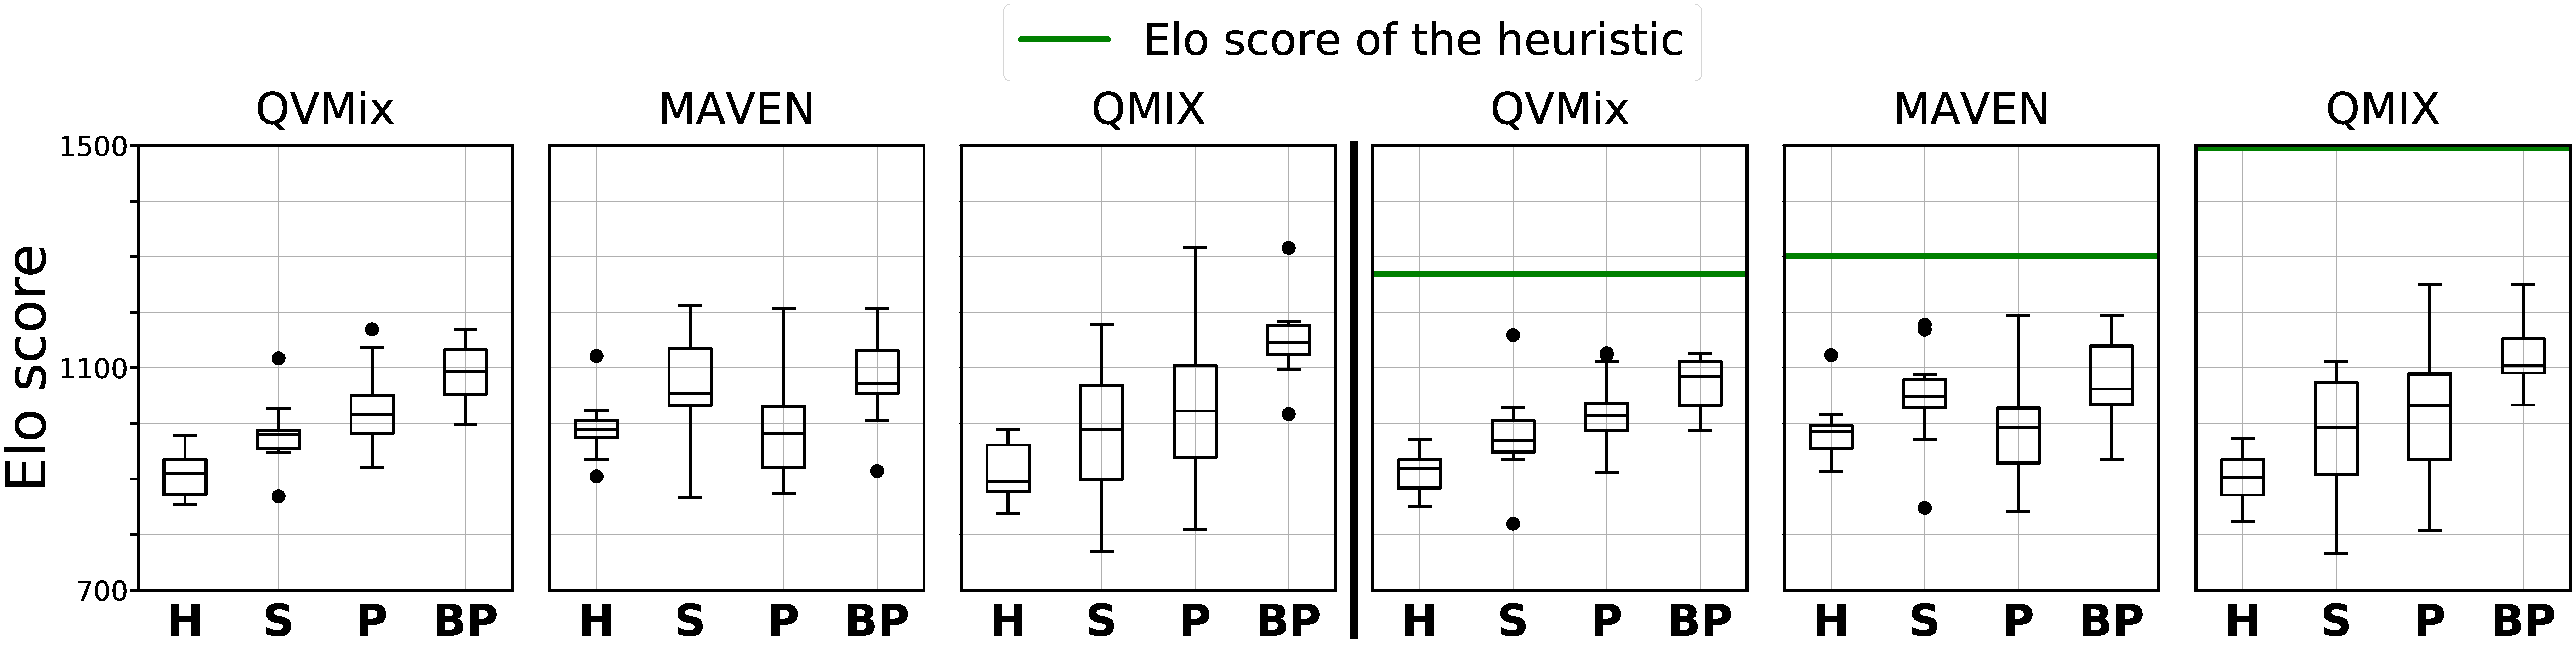
\includegraphics[width=\textwidth]{tex_thesis/figures/ch7/3s5z_tiny_six_qvmix_maven_qmix.pdf}
    \begin{subfigure}{.045\textwidth}
    \centering
    \caption*{}
    \end{subfigure}%
    \begin{subfigure}{.455\textwidth}
        \begin{subfigure}{.33\textwidth}
            \renewcommand\thesubfigure{\alph{subfigure}.1}
          \centering
          \caption{}
          \label{subfig:3s5z_elo_no_h_methodQVMIX}
        \end{subfigure}%
        \begin{subfigure}{.33\textwidth}
        \addtocounter{subfigure}{-1}
            \renewcommand\thesubfigure{\alph{subfigure}.2}
          \centering
          \caption{}
          \label{subfig:3s5z_elo_no_h_methodMAVEN}
        \end{subfigure}%
        \begin{subfigure}{.33\textwidth}
        \addtocounter{subfigure}{-1}
            \renewcommand\thesubfigure{\alph{subfigure}.3}
          \centering
          \caption{}
          \label{subfig:3s5z_elo_no_h_methodQMIX}
        \end{subfigure}%
    \centering
    \addtocounter{subfigure}{-1}
    \caption{$3s5z$ map \textbf{without} heuristic.}
     \label{subfig:elo_no_h_3s5z}
    \end{subfigure}%
    \begin{subfigure}{.455\textwidth}
        \begin{subfigure}{.33\textwidth}
        \renewcommand\thesubfigure{\alph{subfigure}.1}
          \centering
          \caption{ }
          \label{subfig:3s5z_elo_h_methodQVMIX}
        \end{subfigure}%
        \begin{subfigure}{.33\textwidth}
         \addtocounter{subfigure}{-1}
        \renewcommand\thesubfigure{\alph{subfigure}.2}
          \centering
          \caption{ }
          \label{subfig:3s5z_elo_h_methodMAVEN}
        \end{subfigure}%
        \begin{subfigure}{.33\textwidth}
            \addtocounter{subfigure}{-1}
            \renewcommand\thesubfigure{\alph{subfigure}.3}
          \centering
          \caption{ }
          \label{subfig:3s5z_elo_h_methodQMIX}
        \end{subfigure}%
    \centering
    \addtocounter{subfigure}{-1}
    \caption{$3s5z$ map \textbf{with} heuristic.}
     \label{subfig:elo_h_3s5z}
    \end{subfigure}%
    
    \caption{Elo score box plots of 12 test populations. 
    Half of the experiments were performed in the $3m$ map, shown at the top (\ref{subfig:elo_no_h_3m}, \ref{subfig:elo_h_3m}) and the other half in the $3s5z$ map, shown at the bottom (\ref{subfig:elo_no_h_3s5z}, \ref{subfig:elo_no_h_3s5z}). 
    In each test population, teams are trained with the same method, which is either QVMix (\ref{subfig:elo_no_h_methodQVMIX}, \ref{subfig:elo_h_methodQVMIX},\ref{subfig:3s5z_elo_no_h_methodQVMIX}, \ref{subfig:3s5z_elo_h_methodQVMIX}), MAVEN (\ref{subfig:elo_no_h_methodMAVEN}, \ref{subfig:elo_h_methodMAVEN},\ref{subfig:3s5z_elo_no_h_methodMAVEN}, \ref{subfig:3s5z_elo_h_methodMAVEN}) or QMIX (\ref{subfig:elo_no_h_methodQMIX}, \ref{subfig:elo_h_methodQMIX},\ref{subfig:3s5z_elo_no_h_methodQMIX}, \ref{subfig:3s5z_elo_h_methodQMIX}).
    In \ref{subfig:elo_h_3m} and \ref{subfig:elo_h_3s5z}, the heuristic is present in the test population and a green line represents its Elo score.
    Box plots represent the distribution of the ELO scores of the teams trained either against the heuristic (\textbf{H}), in self-play (\textbf{S}), within a population (\textbf{P}) or the best of each training population (\textbf{BP}).
    For most methods, teams trained within a population achieved the highest Elo scores.
    Box plots present the median, the first quantile ($Q1$) and the third quantile ($Q3$). The reach of whiskers is defined by $1.7*(Q3-Q1)$.
    }
    \label{fig:elo_method}

 
\end{figure*} 

The same experiment is performed with the addition of the heuristic in the three test populations and corresponding box plots are presented in Figures \ref{subfig:elo_h_3m} and \ref{subfig:elo_h_3s5z}.
The heuristic scores are different depending on the map.
In the $3m$ map, most of the teams achieve a higher Elo score than the heuristic, whereas in $3s5z$, the heuristic dominates all teams.
In the $3s5z$ map and for all three learning scenarios, Elo scores slightly decreased with the addition of the heuristic.
The conclusion is straightforward and the heuristic is better than all teams.
However, one should note that the score ordering between the teams remained the same between Figure \ref{subfig:elo_no_h_3s5z} and \ref{subfig:elo_h_3s5z}.
In $3m$, one can see that the Elo score of teams trained against the heuristic (\textbf{H}) is higher in Fig. \ref{subfig:elo_h_3m} than the ones in Figure \ref{subfig:elo_no_h_3m}, as a direct consequence of the introduction into the test populations of a team against which they win.
When compared with the previous test populations (Fig. \ref{subfig:elo_no_h_3m}), teams trained with QVMix achieved higher Elo scores than without the heuristic in the test population (Fig. \ref{subfig:elo_h_methodQVMIX}), while when trained with MAVEN and QMIX, they achieved lower Elo scores (Fig. \ref{subfig:elo_h_methodMAVEN}, \ref{subfig:elo_h_methodQMIX}).
In all cases, the higher values of box plots are not significantly different but lower values are, meaning that some teams performed poorly against the heuristic.
The conclusion is that teams trained within a population remain the most successful in most of our experiments, no matter if the heuristic is the best or almost the worst team.

\begin{figure*}
    
\begin{subfigure}{\textwidth}
\centering
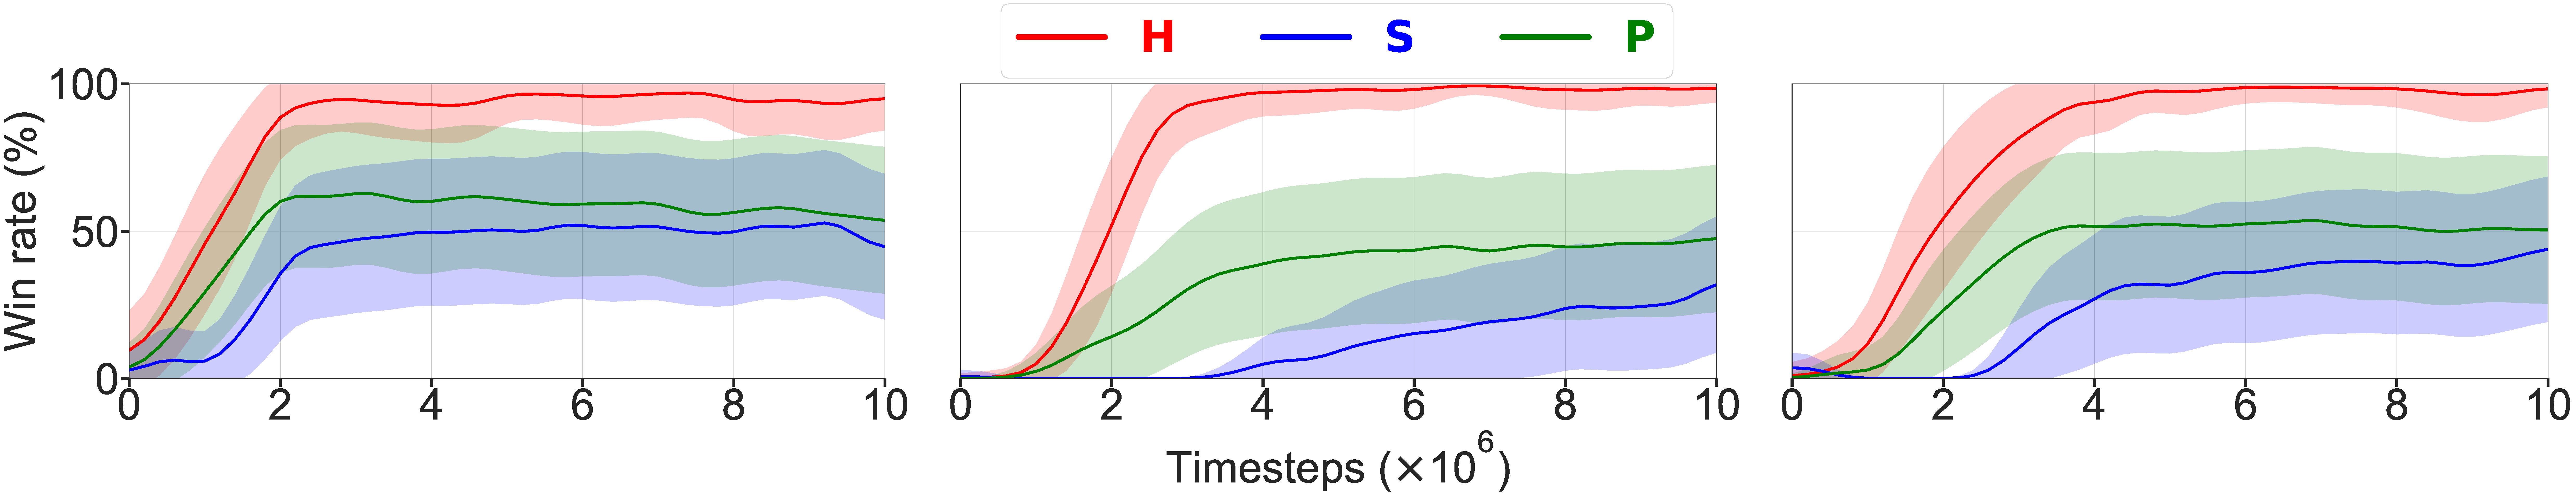
\includegraphics[width=.95\textwidth]{tex_thesis/figures/ch7/tiny_heuristic_plot_qvmixmavenqmix.pdf}
    \begin{subfigure}{.05\textwidth}
    \centering
    \caption*{}
    \end{subfigure}%
    \begin{subfigure}{.31\textwidth}
    \renewcommand\thesubfigure{\alph{subfigure}.1}
      \centering
      \caption{QVMix}
      \label{subfig:vs_h_methodQVMIX}
    \end{subfigure}%
    \begin{subfigure}{.31\textwidth}
    \addtocounter{subfigure}{-1}
    \renewcommand\thesubfigure{\alph{subfigure}.2}
      \centering
      \caption{MAVEN}
      \label{subfig:vs_h_methodMAVEN}
    \end{subfigure}%
    \begin{subfigure}{.31\textwidth}
    \addtocounter{subfigure}{-1}
    \renewcommand\thesubfigure{\alph{subfigure}.3}
      \centering
      \caption{QMIX}
      \label{subfig:vs_h_methodQMIX}
    \end{subfigure}
\addtocounter{subfigure}{-1}
\caption{Win rates achieved against the heuristic in the $3m$ map.}    
\label{subfig:3m_vs_h}
\end{subfigure}
\begin{subfigure}{\textwidth}
    \centering
    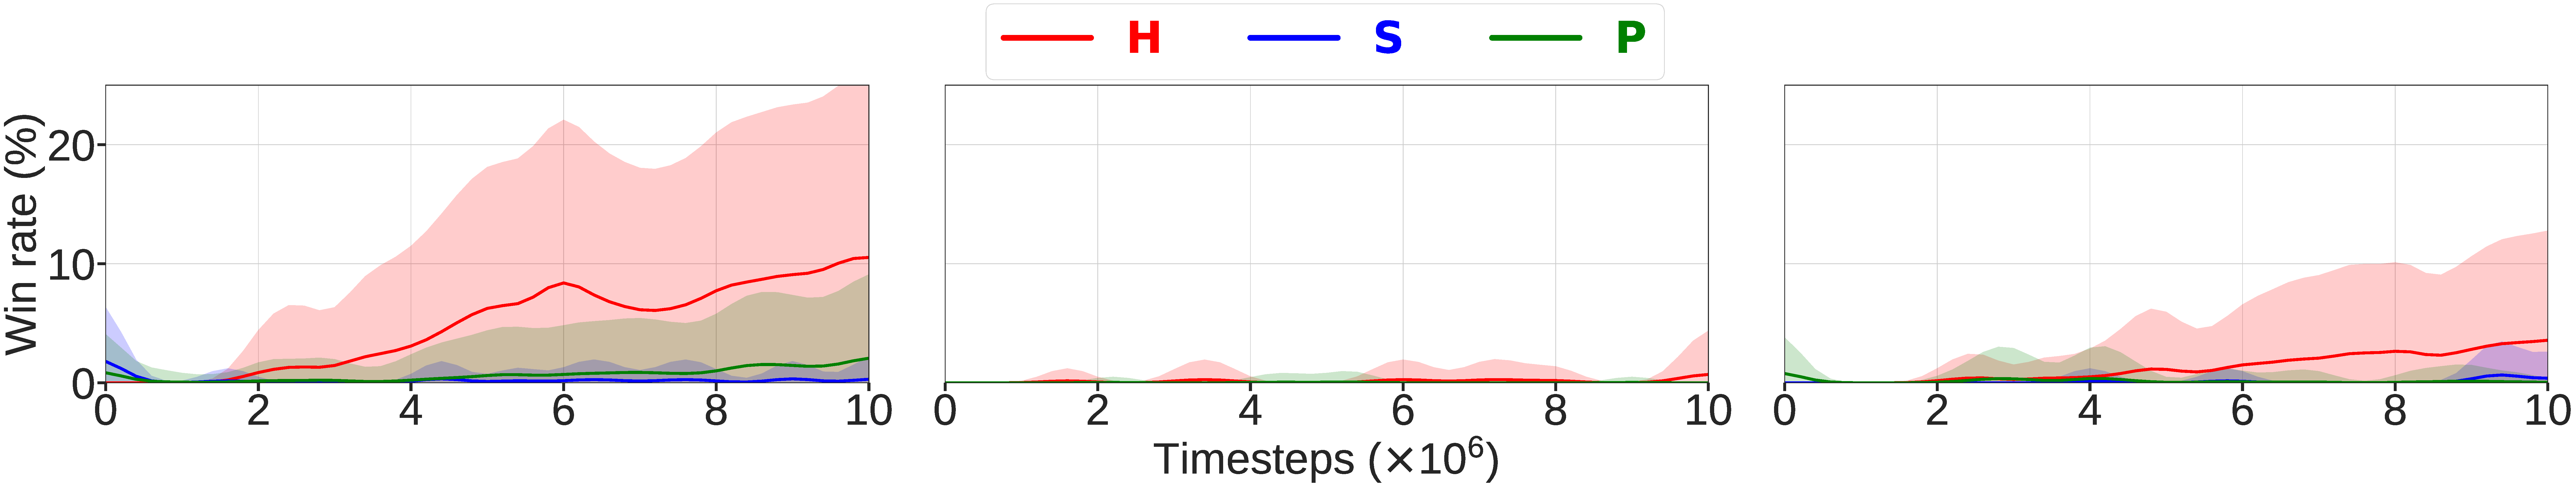
\includegraphics[width=.95\textwidth]{tex_thesis/figures/ch7/3s5z_tiny_heuristic_plot_qvmixmavenqmix.pdf}
    \begin{subfigure}{.05\textwidth}
    \centering
    \caption*{}
    \end{subfigure}%
    \begin{subfigure}{.31\textwidth}
    \renewcommand\thesubfigure{\alph{subfigure}.1}
      \centering
      \caption{QVMix}
      \label{subfig:3s5z_vs_h_methodQVMIX}
    \end{subfigure}%
    \begin{subfigure}{.31\textwidth}
    \addtocounter{subfigure}{-1}
    \renewcommand\thesubfigure{\alph{subfigure}.2}
      \centering
      \caption{MAVEN}
      \label{subfig:3s5z_vs_h_methodMAVEN}
    \end{subfigure}%
    \begin{subfigure}{.31\textwidth}
    \addtocounter{subfigure}{-1}
    \renewcommand\thesubfigure{\alph{subfigure}.3}
      \centering
      \caption{QMIX}
      \label{subfig:3s5z_vs_h_methodQMIX}
    \end{subfigure}
\addtocounter{subfigure}{-1}
\caption{Win rates achieved against the heuristic in the $3s5z$ map. Note the change in scale of the y-axis.}
\label{subfig:3s5z_vsh}
\end{subfigure}
\begin{subfigure}{\textwidth}
\centering
    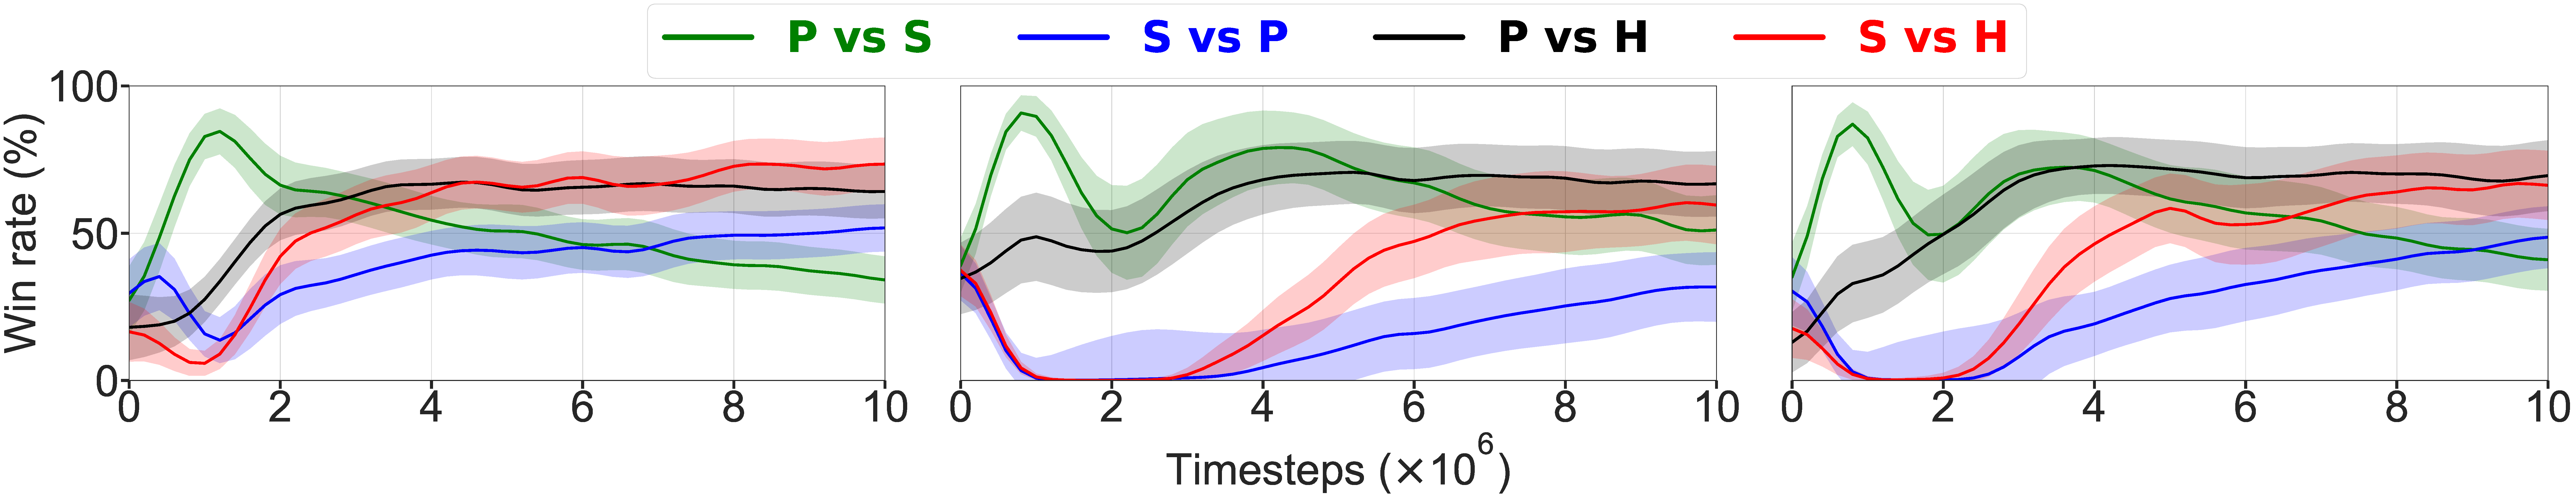
\includegraphics[width=.95\textwidth]{tex_thesis/figures/ch7/tiny_perf_self_popu.pdf}
    \begin{subfigure}{.05\textwidth}
    \centering
    \caption*{}
    \end{subfigure}%
    \begin{subfigure}{.31\textwidth}
    \renewcommand\thesubfigure{\alph{subfigure}.1}
      \centering
      \caption{QVMix}
      \label{subfig:duo_methodQVMIX}
    \end{subfigure}%
    \begin{subfigure}{.31\textwidth}
    \addtocounter{subfigure}{-1}
    \renewcommand\thesubfigure{\alph{subfigure}.2}
      \centering
      \caption{MAVEN}
      \label{subfig:duo_methodMAVEN}
    \end{subfigure}%
    \begin{subfigure}{.31\textwidth}
    \addtocounter{subfigure}{-1}
    \renewcommand\thesubfigure{\alph{subfigure}.3}
      \centering
      \caption{QMIX}
      \label{subfig:duo_methodQMIX}
    \end{subfigure}
\addtocounter{subfigure}{-1}
\caption{Win rates achieved by teams trained in the $3m$ map against themselves.}
\label{subfig:3m_duo}
\end{subfigure}
\begin{subfigure}{\textwidth}
\centering
    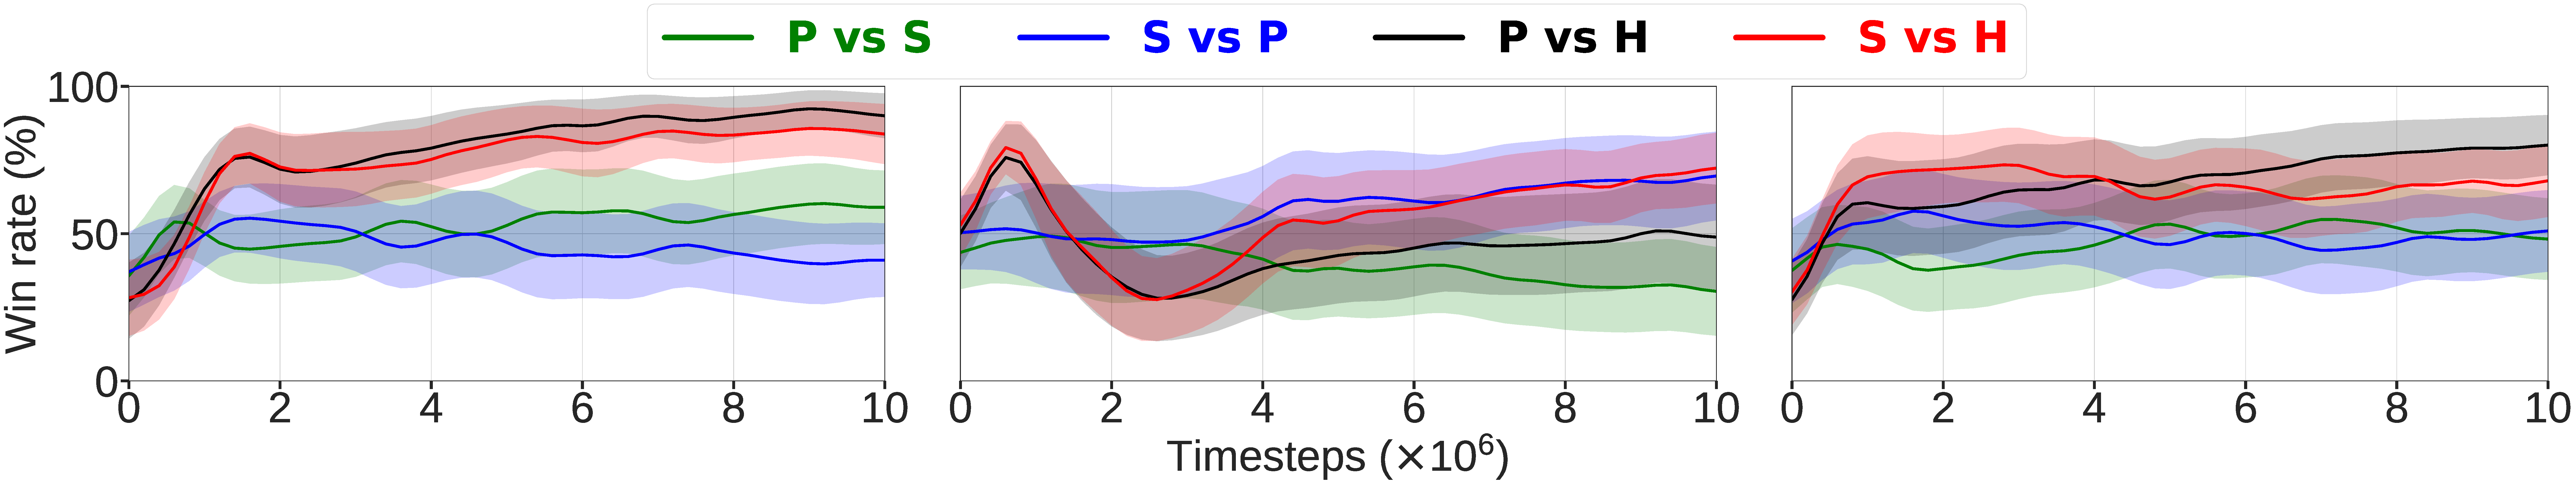
\includegraphics[width=.95\textwidth]{tex_thesis/figures/ch7/3s5z_tiny_perf_self_popu.pdf}
    \begin{subfigure}{.05\textwidth}
    \centering
    \caption*{}
    \end{subfigure}%
    \begin{subfigure}{.31\textwidth}
    \renewcommand\thesubfigure{\alph{subfigure}.1}
      \centering
      \caption{QVMix}
      \label{subfig:3s5z_duo_methodQVMIX}
    \end{subfigure}%
    \begin{subfigure}{.31\textwidth}
    \addtocounter{subfigure}{-1}
    \renewcommand\thesubfigure{\alph{subfigure}.2}
      \centering
      \caption{MAVEN}
      \label{subfig:3s5z_duo_methodMAVEN}
    \end{subfigure}%
    \begin{subfigure}{.31\textwidth}
    \addtocounter{subfigure}{-1}
    \renewcommand\thesubfigure{\alph{subfigure}.3}
      \centering
      \caption{QMIX}
      \label{subfig:3s5z_duo_methodQMIX}
    \end{subfigure}
\addtocounter{subfigure}{-1}
\caption{Win rates achieved by teams trained in the $3s5z$ map against themselves.}
\label{subfig:3s5z_duo}
\end{subfigure}

\caption{
Means of win rate achieved along training time steps by confronting teams trained with the same method against the heuristic or against other teams trained with a different learning scenario.
Teams are trained either with QVMix, MAVEN, or QMIX.
Tests were performed in the $3m$ map, shown at the top, and in the $3s5z$ maps, shown at the bottom. 
Win rates against the heuristic are presented in red, blue and green for teams trained against the heuristic, in self-play and within a population, respectively.
Win rates of teams trained within a population against teams trained in self-play are presented in green and against teams trained against the heuristic in black.
Win rates of teams trained in self-play against teams trained within a population are presented in blue and against teams trained against the heuristic in red.
The error band is half the standard deviation.
} 
\label{fig:heuristic_plot}
\end{figure*}


In Figure \ref{subfig:3m_vs_h}, we present the evolution of win rates against the heuristic along training timesteps by each team in the $3m$ map.
For all methods, teams trained against the heuristic are the best against it on average.
This explains why their Elo scores improve when the heuristic is included in the test population.
This is also the case for QVMix teams trained in self-play and within a population that performed better and learned faster than teams trained with MAVEN and QMIX with these two learning scenarios.
However, in the $3s5z$ map, it can be seen in Figure \ref{subfig:3s5z_vsh} that the win rates against the heuristic are very low, not to say equal to zero.
Only the win rates of teams trained against the heuristic, especially with QVMix and QMIX, increase at the end of the training but with a high variance in comparison to the $3m$ map (Fig. \ref{subfig:3m_vs_h}).
For QVMix, the win rates of teams trained with a population also increase at the end of the training phase.
The time we have budgeted for training in the $3s5z$ map may be insufficient to achieve a high win rate.
However, we find this beneficial because it shows that, even when the heuristic is better than all teams, training against it, with the same training timesteps allowance, is not the best learning scenario when teams have to be good against several strategies.
This also shows that our heuristic is harder to defeat with respect to the results of \citep{Rashid2018,Mahajan2019MAVEN:Exploration,leroy2020qvmix} where better results are observed in these maps with the former SMAC heuristic.

In the $3m$ map, the standard deviation of green and blue win rates, representing population and self-play learning scenarios respectively, is high and confirms the results of Elo score box plots that there are performance gaps between teams trained within the same learning scenario.
Observations also suggest that teams trained in self-play would achieve the same win rates as teams trained within a population if they were trained for longer, suggesting a difference of training sample efficiency.
As teams first need to learn to cross the map to meet opponents and to learn to fight them, this difference is because training within a population, against several strategies, increases the probability of creating episodes where two opposing agents meet and fight at the beginning of training.

Win rates from the confrontations between trained teams are presented in Figures \ref{subfig:3m_duo} and \ref{subfig:3s5z_duo}.
The draw rates can be obtained by subtracting from $1$ the sum of these two curves.
This confirms the previous results with box plots that training against the heuristic is the worst scenario, as an average win rate above $60\%$ is achieved against them as shown in the black and red curves.
Green and blue curves enable one to analyse self-play against population-learning scenarios.
At the beginning of the training phase, teams trained within a population are better than self-play ones in the $3m$ map.
This high win rate decreases with training in favour of the win rate of teams trained in self-play, and for QVMix and QMIX, until it becomes higher than the latter.
Again, this suggests a difference in training sample efficiency.
Moreover, although the training sample efficiency is lower for teams trained in self-play, the number of environment timesteps required to train them is five-times lower in our setting.
However, it is, on average, that the self-play teams become better.
In the $3s5z$ map, this overlap phenomenon does not occur and the average win rates fluctuate around $50\%$ with the green curves remaining just above the blue ones at the end.
The proximity of performances between teams trained in self-play and within a population is arguably due to the environment and the $3m$ map which does not offer the possibility of winning with very different strategies.
As the $3s5z$ map appears to be more complex, with the lack of performances against the heuristic as evidence, teams trained within a population remain better on average.

On average, the results of the teams trained within a population with MAVEN in the 3s5z map differ from the other experiments. 
Some results are slightly worse in regard to those of the other experiments.
The reason for this is not clear, as we executed the experiments several times, but this does not affect the conclusions of our experiments that remain clear.
Finally, it would be necessary to repeat these experiments more times or to analyse the behaviour of the agents in depth to find the problem, which is beyond the scope of this paper. 

In Figure \ref{fig:all}, we present the box plots of Elo scores obtained by all trained teams and the heuristic in a single test population for both maps.
We observe that the learning scenario ranking remains the same as in other experiments.
In the $3m$ map, QMIX achieves the highest Elo scores while the lowest MAVEN Elo scores are worse than the ones of QMIX and QVMix when teams are trained in self-play or within a population.
QVMix produces results with a lower variance than QMIX.
In the $3s5z$ map, QVMix is the one achieving the highest Elo scores and it is also MAVEN that achieves the lowest ones.
We conducted the same experiment without the heuristic, which led to the same conclusion (see Figure \ref{fig:all_no_h} in Appendix \ref{app:all_no_h}).
Despite its mechanism of exploration, MAVEN is not able to outperform QMIX and QVMix.
This is also the case in \citep{Mahajan2019MAVEN:Exploration} and \citep{leroy2020qvmix} where they show that MAVEN outperforms QMIX but not QVMix in more complex Dec-POMDP environments.

\begin{figure*}[ht]
\begin{subfigure}{\textwidth}
\centering
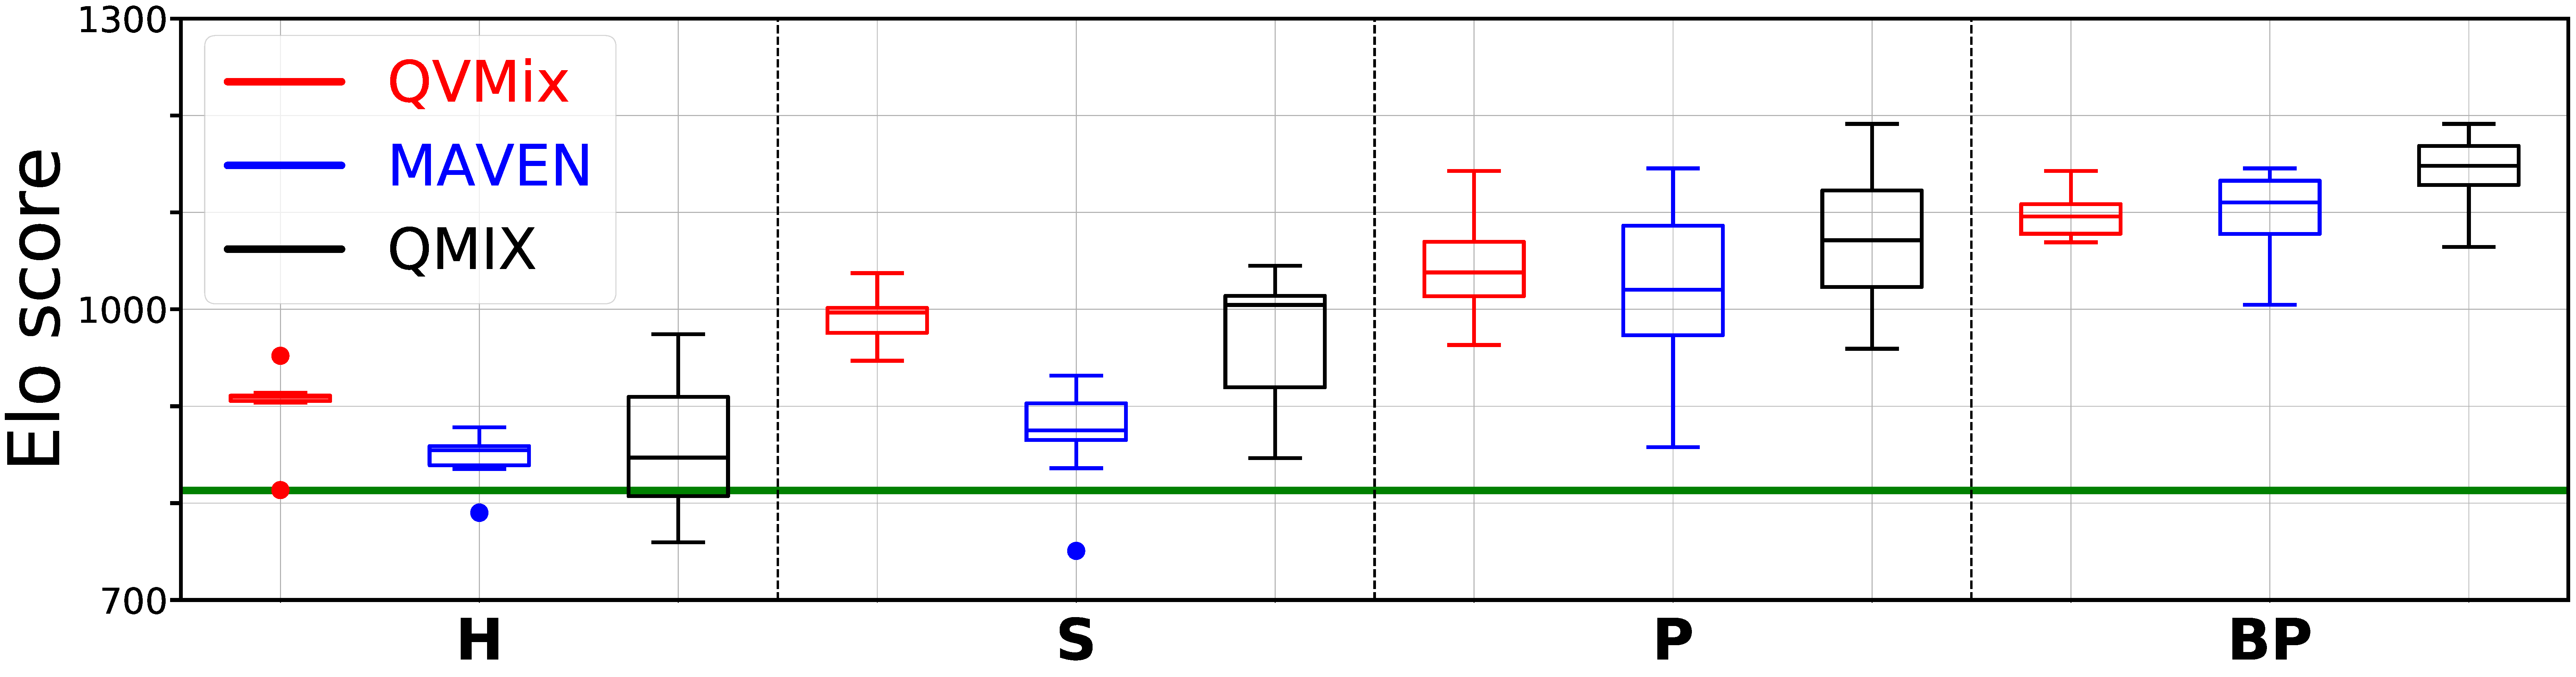
\includegraphics[width=.95\textwidth]{tex_thesis/figures/ch7/3m_tiny_all_h_clean.pdf}
\caption{$3m$}
\label{subfig:3m_all_h}
\end{subfigure}
\begin{subfigure}{\textwidth}
\centering
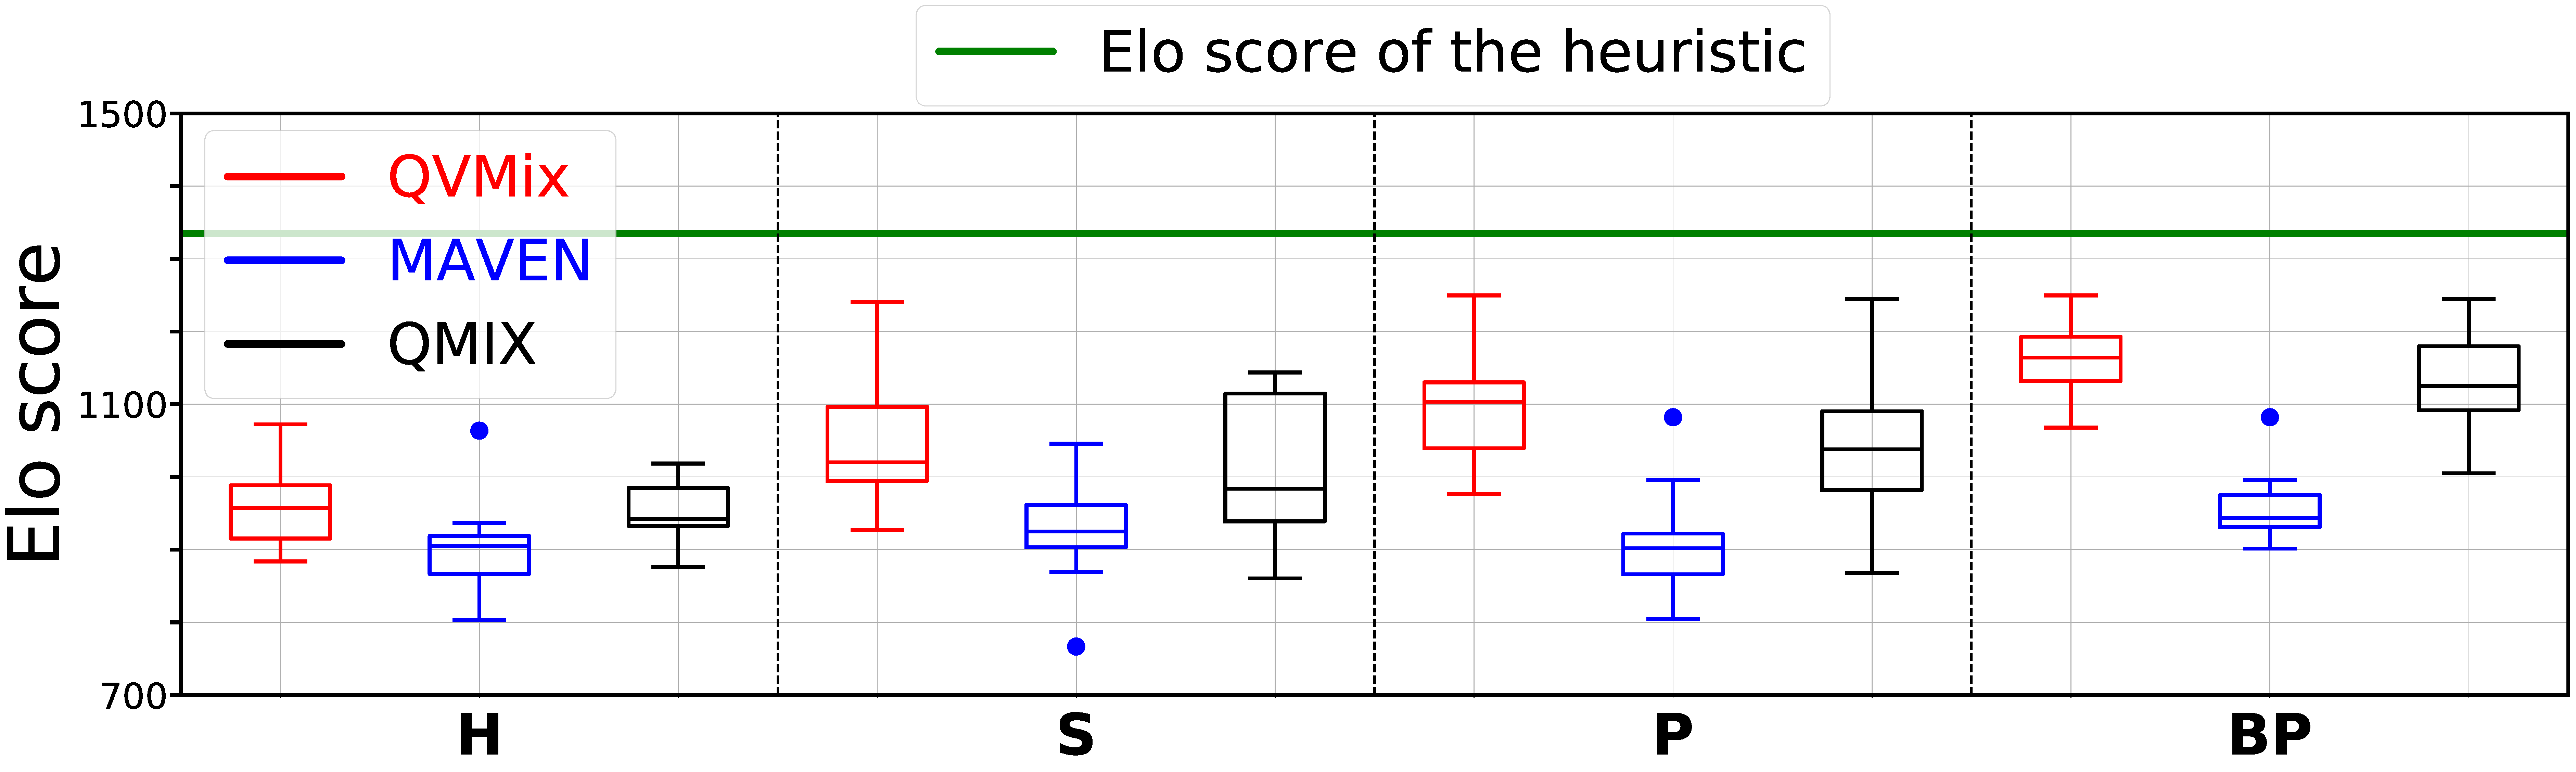
\includegraphics[width=.95\textwidth]{tex_thesis/figures/ch7/3s5z_tiny_all_h_clean.pdf}
\caption{$3s5z$}
\label{subfig:3s5z_all_h}
\end{subfigure}
\caption{
Elo score box plots of two test populations, in $3m$ at the top and in $3s5z$ at the bottom, composed of the heuristic and teams trained using three methods and three learning scenarios.
The training method is either QVMix (red), MAVEN (blue) or QMIX (black).
Box plots represent the distribution of the ELO scores of teams trained either against the heuristic (\textbf{H}), in self-play (\textbf{S}), within a population (\textbf{P}) or the best of each population (\textbf{BP}).
Box plots present the median, the first quantile ($Q1$) and the third quantile ($Q3$). The reach of whiskers is defined by $1.7*(Q3-Q1)$.
}
\label{fig:all}
\end{figure*}

\begin{figure*}[ht]
\centering

\begin{subfigure}{\textwidth}
\centering
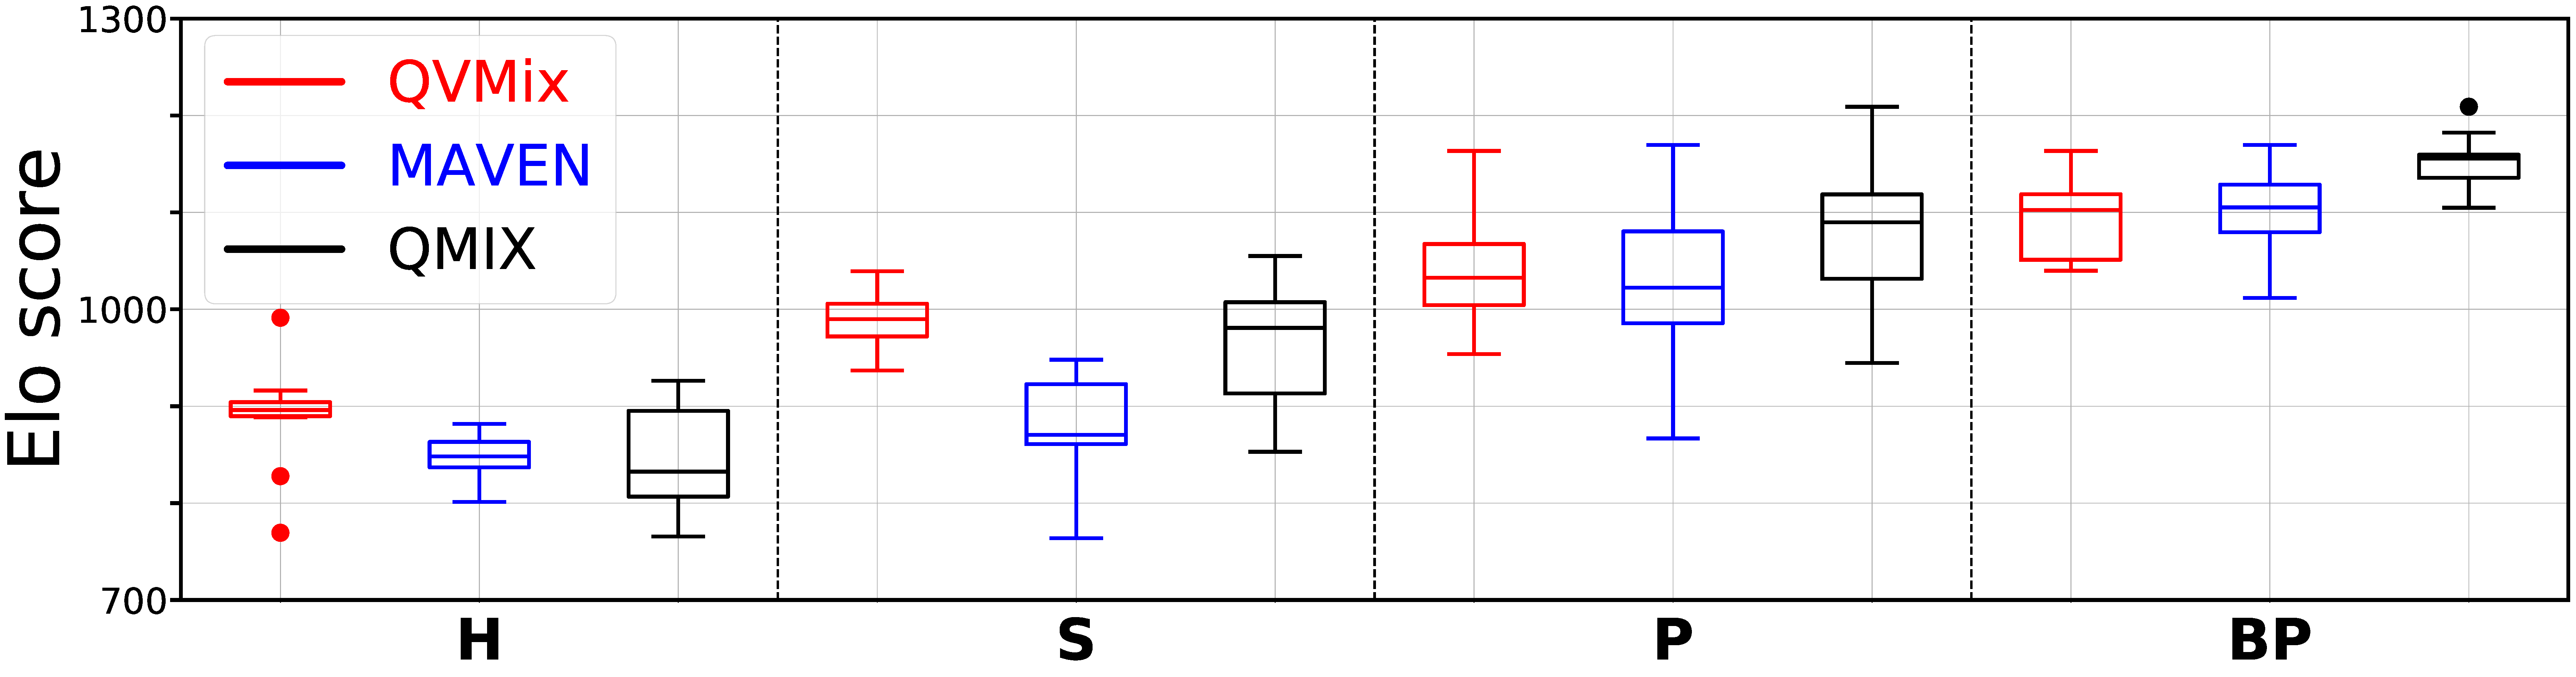
\includegraphics[width=\textwidth]{tex_thesis/figures/ch7/3m_tiny_all_no_h_clean.pdf}
\caption{$3m$}
\label{subfig:3m_all_no_h}
\end{subfigure}
\begin{subfigure}{\textwidth}
\centering
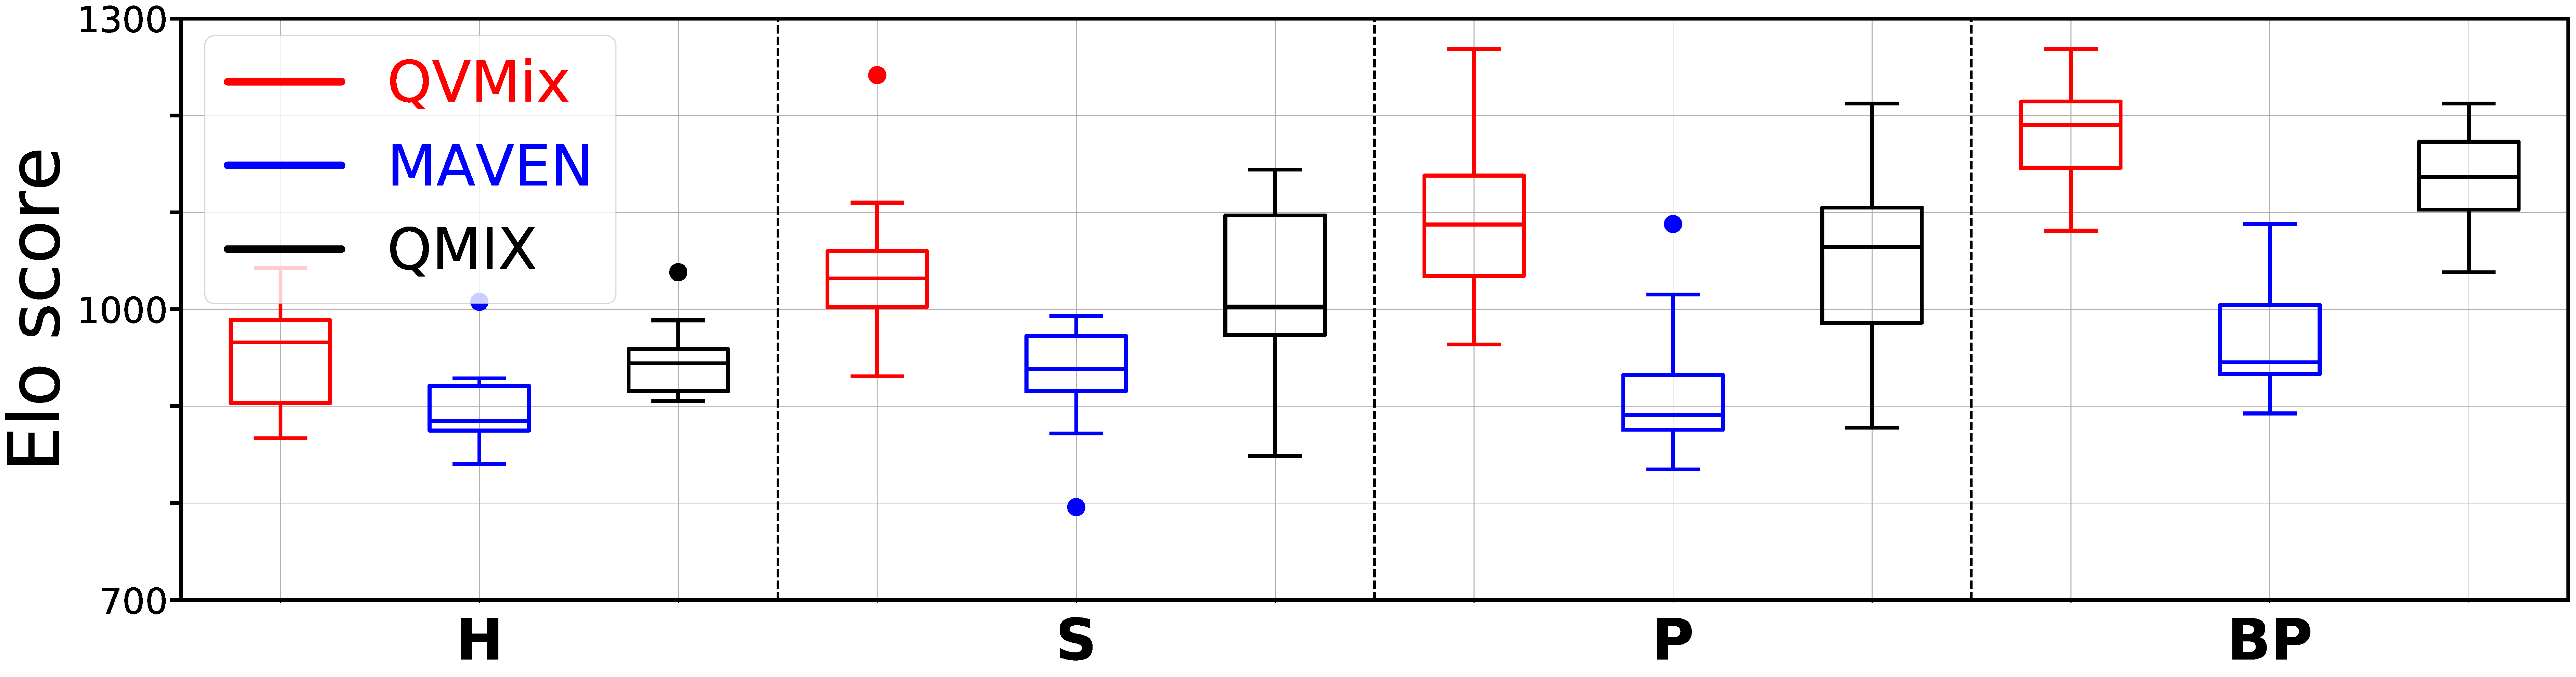
\includegraphics[width=\textwidth]{tex_thesis/figures/ch7/3s5z_tiny_all_no_h_clean.pdf}
\caption{$3s5z$}
\label{subfig:3s5z_all_no_h}
\end{subfigure}
\caption{
Elo score box plots of two test populations, in $3m$ at the top and in $3s5z$ at the bottom, composed of teams trained using three methods and three learning scenarios.
The training method is either QVMix (red), MAVEN (blue) or QMIX (black).
Box plots represent the distribution of the Elo scores of teams trained either against the heuristic (\textbf{H}), in self-play (\textbf{S}), within a population (\textbf{P}) or the best of each population (\textbf{BP}).
Box plots present the median, the first quantile ($Q1$) and the third quantile ($Q3$). The reach of whiskers is defined by $1.7*(Q3-Q1)$.
}
\label{fig:all_no_h}
\end{figure*}



\section{Related work}
\label{sec:related}
Close to our work, Phan et.al. \citep{phan2020learning} proposed the antagonist-ratio training scheme (ARTS) to train a team to be resilient to failures.
To improve resilience of cooperative methods, they simulate failures as a mixed cooperative-competitive setting where the faulty agents are adversarial agents of another team.
As in our work, ARTS combines CTDE methods, such as QMIX, and population based training.

In this paper, we consider three CTDE value-based methods QMIX \citep{Rashid2018}, MAVEN \citep{Mahajan2019MAVEN:Exploration} and QVMix \citep{leroy2020qvmix} designed for Dec-POMDP.
They rely on the same factorisation of $Q(s, \mathbf{u})$ with a constrained hypernetwork.
This constraint implies representation limits.
Other research papers have sought to change this factorisation and achieved better performances than QMIX.
To cite some, QTRAN \citep{Son2019QTRAN:Learning} factorises it by additive decomposition and QPLEX \citep{wang2021qplex} uses a duplex dueling network architecture, taking advantage of the dueling architecture \citep{wang2016dueling}, to learn both $Q(s, \mathbf{u})$ and $Q_a$.
In parallel, others have succeeded to remove the factorisation, such as LAN \citep{avalos2021local} which also take advantage of the dueling architecture \citep{wang2016dueling} to learn a centralised value function with independent advantage functions.
Policy-based methods is another family of RL methods that have inspired many CTDE algorithms, such as COMA \citep{Foerster2017}, MADDPG \citep{lowe2017multi}, LIIR \citep{Du2019LIIRLearning}, FACMAC \citep{peng2021facmac} and HATPRO, HAPPO \citep{kuba2021trust}.


As introduced, self-play or population based training for competitive settings have already been explored in many works \citep{jaderberg2019human, vinyals2019grandmaster, baker2019emergent}.
More advanced techniques have been widely studied in the literature such as fictitious play \cite{brown1951iterative} or best response dynamic \citep{baudin2022fictitious}.
In short, it consists in choosing the policy which is the best response against the average strategy of an opponent.
In self-play, we mention fictitious play to play Poker \citep{pmlr-v37-heinrich15} and Deep Nash to play Stratego \citep{DM_stratego}.
In population based training, we mention policy-space response oracles (PSRO) \citep{NIPS2017_3323fe11, Muller2020A}.
These methods are referred to as opponent modelling.
Extensions of these works consider to additionally learn how the opponent will update its strategy \citep{he2016opponent, foerster2017learning}.
Recently, Tian et. al. \citep{tian2022multi} introduced a time dynamical opponent model to encode opponent policies in a CTDE framework for mixed cooperative-competitive environment.



\section{Discussion and future work}
In this paper, we evaluated learning scenarios to train teams to face multiple strategies in a symmetric two-team Markov game.
Teams are trained with three CTDE value-based methods: QMIX, MAVEN and QVMix and with three learning scenarios differentiated by the variety of strategies that teams will encounter during their training.
Specifically, they are trained by playing against a stationary strategy, against themselves, or within a population of teams trained using the same method.
To perform our experiments, we modified the cooperative environment SMAC to allow teams to compete and train at the same time, and trained teams in two different SMAC environments.
These nine types of trained teams are evaluated at the end of their training with the Elo rating system.
Different groups are formed to identify which learning scenario is the best and which learning scenario/training method pair is the best.
We also analysed the win rates of several matchups during training to support the results provided by the Elo scores.
Our results showed that training teams within a population of learning teams is the best learning scenario, when each team plays the same number of timesteps for training purposes.
We reached this conclusion irrespective of whether or not the stationary strategy was better than all trained teams.
Finally, a selection procedure is required because teams from the same training population do not perform equally.


This work is a first investigation of two-team competition with CTDE methods, and we hereafter suggest several future research directions.
First, we suggest to perform the same experiments on more complex environments and to tackle the challenges of an asymmetric two-team Markov games.
In this paper, we selected value-based methods because of their performances in SMAC \citep{samvelyan2019starcraft} at the time of our experiments.
Recent CTDE methods overcome these performances and may lead to interesting new results.
Another research direction would be to study how diversity in the training population impacts the performances. 
Diversity could be increased by adding the heuristic in the population, confronting agents against older learned policies, varying the size of the population or training teams with different methods in the same population.
In addition, as described in Section \ref{sec:related}, methods that compute best responses or model the opponent are widely studied in the literature and would be interesting to test in such environment.
We also propose performing behavioural and policy analyses so as to better understand why some teams achieve a better Elo score and how different are strategies in a single training population.

\todo{Check figure are the same and no problem at import}\cleardoublepage
\part{Conclusion}\label{part:conclusion}
\chapter{Conclusion}\label{ch:conclusion}

This thesis demonstrates through three contributions the usefulness of considering other learning agents when training one with reinforcement learning in a multi-agent environment.
We provide the necessary background before presenting three specific contributions.
The first contribution extends the DQV single-agent algorithms to cooperative multi-agent ones, outperforming the methods compared against.
The second contribution demonstrates the interest of these cooperative methods in the context of a real-world application: the infrastructure management problem.
The third contribution analyses how to train a team in a mixed cooperative-competitive setting where two teams compete.
We hereafter summarise the three parts of this chapter and discuss the scientific findings before finally discussing the potential societal impact of multi-agent reinforcement learning.

Part \ref{part:background} provides the required background to understand the successive parts.
Specifically, Chapter \ref{ch:background} presents the stochastic game, a general framework for multi-agent reinforcement learning and how it can be adapted when considering specific settings.
Multi-agent reinforcement learning takes its foundation in single-agent reinforcement learning, and we offer a succinct introduction to its basics.
Specifically, we discuss model-based and dynamic programming, focus on value-based and policy-based methods for model-free RL and conclude by addressing the partial observability of agents.

Part \ref{part:coop} tackles the problem of training agents to learn to cooperate.
When agents cooperate, the setting can be framed as a decentralised partially observable Markov decision process where agents share the same reward.
This part comprises three chapters.
One is a background chapter, and the others highlight two specific contributions.

Chapter \ref{ch:cooperation} defines the cooperative framework and applications that can be framed as such a problem.
Several cooperative MARL methods to solve Dec-POMDP are defined following its definition, emphasising how algorithms have been designed to allow centralised training with decentralised execution.
While we postpone comparing the performance of these methods to later chapters, this third chapter concludes with a literature discussion, highlighting works that are not considered in this manuscript but are of interest.

Chapter \ref{ch:qvmix} presents QVMix and other value-based methods for Dec-POMDP.
It highlights that learning the state value function along the state-action value function as it is done in SARL by the DQV family of algorithms can be extended to cooperative CTDE methods in MARL.
Moreover, it allows to outperform the methods compared against and to not overestimate the state-action value function unlike these compared value-based methods relying on the classical Q-learning update.

Chapter \ref{ch:impmarl} concludes Part \ref{part:coop} by presenting infrastructure management planning, a real-world application that can be framed as a Dec-POMDP.
Managing infrastructure by timely inspecting or repairing system components to minimise failure risk and maintenance cost becomes challenging as the system grows in size.
Decentralising the decision, making each component an independent agent, and training them with CTDE methods allows for scaling to large systems.
Framing it as a multi-agent problem allows it to scale and to outperform rule-based approaches, considered the state-of-the-art for solving these problems.

Part \ref{part:compet} tackles training agents to learn to cooperate when competing against another team.
This mixed cooperative-competitive setting requires to benefit from the methods used to train agents from one team to cooperate along with the training scenarios required to train an agent in a competitive environment.
This part is divided into two chapters. 
The former provides background on the competition setting, while the latter presents specific contributions where we trained teams to compete against each other.

Chapter \ref{ch:competition} addresses challenges when agents do not purely cooperate.
This is the case not only in competitive settings but also in general-sum ones.
This chapter presents different types of solutions that game theory provides because Nash equilibrium is not the single one.
Following this, we discuss historical methods for computing these solutions, from dynamic programming to planning methods.
The chapter concludes with the presentation of self-play and population training, two popular training scenarios for training agents in competitive or general-sum environments.

Chapter \ref{ch:2teams} presents a study to train one team of agents to compete against another.
This setting is a symmetric two-team Markov game where two teams composed of the same agents compete.



is the third background chapter focusing on the competition scenario.
The different types of solution in multi-agent system provided by game theory are reviewed.\cleardoublepage

\addtocontents{toc}{\protect\vspace*{\baselineskip}\protect}
\cleardoublepage
\makeatletter
\def\toclevel@chapter{-1}
\makeatother



% Back pages ==================================================================
\appendix
\part{Appendix}
\chapter{Supplementary materials} \label{ch:ch5_appendix}
\section{IMP-MARL public repository, license, data, and documentation}
\label{sec:ch5_appendix_imp_public_repo}
% Repository license and instructions
IMP-MARL's suite of environments is publicly available on the GitHub repository \url{https://github.com/moratodpg/imp\_marl}, featuring an open-source Apache v2 license.  Moreover, IMP-MARL contains wrappers to facilitate its implementation on typical MARL ecosystems, i.e., Gym \citep{openaigym}, RLLib \citep{liang2018rllib}, and PyMarl \citep{samvelyan2019starcraft}, as detailed in Section \ref{sec:experiments}.
% How to reproduce the results
To reproduce the work reported in this paper, the following process can be executed: (i) cloning the repository, (ii) installing a virtual environment with the package requirements, and (iii) executing the script instructions of the corresponding method and IMP-MARL environments.
In addition to the instructions for reproducing our results, we also provide tutorials to add new environments or wrappers.
% How to directly download the results % How to download controllers
We also provide the data files resulting from our experiments, enabling the reproduction of any reported result without re-running the experiments, as well as the corresponding implementation code, hence facilitating future cross-comparisons.
The readily available results include Figures \ref{fig:results}, \ref{fig:learning_curves_cc_false}, and \ref{fig:learning_curves_cc_true}, along with Tables \ref{tab:koutofnresults}, \ref{tab:correlatedkoutofnresults}, \ref{tab:owfresults}.
Configuration, execution, and results files are permanently stored at Zenodo, accessible via \url{https://zenodo.org/record/8032339}. 
Additionally, the controller networks' weights of the best policies presented in Figure \ref{fig:results} are also stored there, thus fostering further interpretability studies of MARL-based strategies.
The dataset is open-access and registered with the Digital Object Identifier (DOI) 10.5281/zenodo.8032339.
More information and dedicated tutorials can be found on the repository.


\section{Experimental details}
\label{sec:ch5_appendix_exp_details}
\subsection{Description of the parameters set up in the experiments}

\begin{table}
  \caption{Parameters set in our experiments.}
  \label{tab:exp_details_common}
  \centering
  \begin{tabular}{llll}
    \toprule
    Parameter name & Parameters value & Parameter name & Parameters value \\
    \midrule
    $\gamma$ & 0.95 & Time max & 2,050,000 \\
    Target update & 200  & RMS epsilon &  $10^{-5}$ \\
    RMS alpha &  0.99  & Grad norm clip & 10 \\
    Learning rate & 0.0005 &Obs last action & True \\
    Agent network & [] - 64 GRU - [] &Save model interval & 20,000 \\
    \bottomrule
  \end{tabular}
\end{table}


In this section, we provide the information required to reproduce the results reported in this paper.
Since the neural networks are trained via MARL using PyMarl's \citep{samvelyan2019starcraft} library, the parameters are here described following PyMarl's convention.
However, their purpose can be easily deduced from the names themselves.
The experimental parameters set up equal across all experiments are presented in Table \ref{tab:exp_details_common}, while the parameters specific to each method are hereafter detailed.
Note that in Table \ref{tab:exp_details_common}, some parameters are not used by all methods, e.g., RMS parameters. Besides, target update intervals, buffer size, and batch size are specified based on the number of episodes.
When the number of agents increases, we only augment the number of trainable parameters of the mixer/critic networks, while the actor networks and other parameters are not modified.
All the parameters can be found in the configuration files available on the GitHub repository and can be used to launch any of the experiments conducted in this paper.

Regarding the agent network representation for CTDE methods and IQL, it consists of one GRU layer with a hidden state that includes 64 features.
This means that the input is fully connected to the 64 hidden states, which are then fully connected to the outputs, one per action.
We represent it as "[] - 64 GRU - []".
Since the number of actions, and hence the number of outputs, of the DQN network is $3^n$, a network with more representation capacity is needed.
In that case, linear layers, whose number of output features are specified between brackets, are also included in the agent network surrounding the GRU layer.
With $n=2$ or $n=3$ agents, the network is set as "[128] - 128 GRU - [128,64]" while for $n=4$ or $n=5$ agents, it is set as "[256] - 256 GRU - [256,256]".
Note that the linear layers before the GRUs include a Relu activation function and the last taken action is also added to the observation of the agents as an additional input.

As mentioned previously, some parameters are common to almost all methods.
For instance, the optimiser selected is RMSProp for all methods, except for FACMAC, which is trained with ADAM.
In nearly all methods, the buffer stores the latest $2,000$ episodes, and at each episode, $64$ episodes are sampled to update the network.
However, since COMA is an on-policy method, the networks are updated with the episodes just played.
Therefore, in our experiments, COMA's networks are updated every four episodes based on these last experienced ones.
This update is performed four times to ensure a fair amount of network updates with respect to the other methods, which are, in turn, updated every episode.

\begin{table}
    \caption{Exploration parameters.}
    \centering
    \begin{tabular}{llll}
    \toprule
    & Epsilon start & Epsilon finish & Epsilon anneal time \\
    \midrule
    Value-base methods & 0.5  & .01 & 5000\\
    FACMAC & 0.3 & 0.005 & 50000 \\
    \bottomrule
    \end{tabular}
    \label{tab:exloration_param}
\end{table}

During training, the value-based methods rely on an epsilon-greedy policy, whose parameters are specified in Table \ref{tab:exloration_param}, while they act following a greedy policy at testing.
Note, however, that COMA and FACMAC utilise different training policies.
FACMAC samples discrete actions through a Gumbel softmax for its actor, whereas exploration is performed via an epsilon, whose values are specified in Table \ref{tab:exloration_param}.
On the other hand, COMA follows a classic stochastic policy during training.
At the testing stage, FACMAC and COMA select actions adhering to a greedy approach, selecting the action associated with the maximum probability.

In the conducted experiments, the parameters set up in the environments differ with respect to the number of agents and we distinguish three cases (i) $n<=10$, (ii) $n=50$, and (iii) $n=100$.
Starting with QMIX, the parameters are all the same when increasing $n$, except for the architecture of the mixing network, whose embedding size in the middle of the mixer is: (i) $32$, (ii) $64$, and (iii) $128$.
QMIX relies on a double-Q feature, i.e., the loss computed to update $\theta$ differ from the original.
While in the original loss function, the target Q value used for the update is selected with the action that maximises the target Q value parameterised by $\theta'$, in double-Q, the action is the one that maximises the Q value parameterised by $\theta$.
Therefore, we have: $\mathcal{L}(\theta) = \mathbb{E}_{\langle . \rangle\sim B} \big[\big(r_{t} + \gamma Q(s_{t+1}, u*; \theta')- Q(s_{t}, u_{t}; \theta)\big)^{2}\big]$ where $u*=\argmax_u Q(s_{t+1}, u; \theta)$.
This target network is updated every $200$ episodes.
QVMix is a variant of QMIX and the parameter values are similarly specified.
In particular, QVMix contains two networks: (i) a Q network with the same architecture as QMIX, and (ii) a V network that is a copy of the Q network, but with only one output.
As for QPLEX, we try to be close to the parameters selected for the SMAC experiments they conduct in their paper.
When $n$ increases, we change only the attention layer size composed of $a$ layers and $b$ heads.
In particular, we set up (i) $1L4H$, (ii) $2L4H$, and (iii) $2L10H$.
The mixer embedding is $64$ for all experiments.

With respect to COMA, which is an actor-critic method, a few specific parameters should be additionally set up.
The agent network, here denoted as the actor, is the same as for the other previously described.
However, the critic varies with $n$ because the input of the critic becomes rather large, and its architecture is fully linear: (i) [128, 128], (ii) [512, 256, 128, 128], and (iii) [2048, 1024, 512, 256, 128].
A TD-$\lambda$ used to update the critic is set to $0.8$ and the learning rate to train the critic is the same as the one of the actor, specified in Table \ref{tab:exp_details_common}.
In terms of FACMAC, the parameters of interest are those at the critic, as its size increases with the number of agents $n$.
FACMAC features a 2-layer-mixing network and, therefore, we specify the size for both:
(i) 64-64, (ii) 128-64, and (iii) 128-128.
As in COMA, the TD-$\lambda$ parameter is set to $0.8$.
The critic has a target network, similar to those included in value-based methods, that is also updated every 200 episodes with a soft target update with $\tau=0.001$.
Moreover, we follow the optimiser selection made in FACMAC's original paper and used ADAM, with an epsilon equal to $10^{-8}$.

Regarding IQL, which is a decentralised method, the parameters are identical in all tested environments.
IQL also has the double-Q feature activated and learns independently individual Q values via DQN's algorithm.
For DQN, we only run experiments with less than five agents, i.e., $n<=5$.
The main difference between tested environments is the size of their networks. 
Since DQN features $3^n$ outputs, only $64$ GRU cells are not enough in terms of network capacity. 
In our experiments, we increase the network size and confirm that DQN manages to achieve similar results as the other MARL methods.
In DQN, the network architecture is the only parameter that is adjusted with the number of agents $n$.

Finally, we list in Table \ref{tab:n_param_train} the number of trainable parameters of the networks.
The input is slightly different between the tested sets of IMP-MARL environments and, therefore, we show in the table only the parameters for one of them.
Note that there is an agent network taking actions for all agents and we purposely duplicate the agent network row to emphasise that all agent's networks are identical across experiments.

\begin{table}
    \caption{Number of trainable parameters in uncorrelated k-out-of-n systems.}
    \centering
    \begin{tabular}{lllllll}
    \toprule
    Method & Network & $n=3$ & $n=5$ & $n=10$ & $n=50$ & $n=100$ \\
    \midrule
    \multirow{2}{*}{QMIX} & Agent & 27,587 & 27,715 & 28,035 & 30,595 & 33,795 \\
 & Mixer & 18,657 & 41,249 & 133,569 & 5,430,657 & 42,202,113 \\
\multirow{2}{*}{QVMix} & Agent & 27,587 & 27,715 & 28,035 & 30,595 & 33,795 \\
 & Mixer & 64,771 & 110,083 & 295,043 & 10,891,779 & 84,437,891 \\
\multirow{2}{*}{QPLEX} & Agent & 27,587 & 27,715 & 28,035 & 30,595 & 33,795 \\
 & Mixer & 58,249 & 83,289 & 155,269 & 1,830,933 & 4,901,797 \\
\multirow{2}{*}{COMA} & Agent & 27,587 & 27,715 & 28,035 & 30,595 & 33,795 \\
 & Critic & 35,971 & 45,955 & 70,915 & 1,195,907 & 10,840,323 \\
\multirow{2}{*}{FACMAC} & Agent & 27,587 & 27,715 & 28,035 & 30,595 & 33,795 \\
 & Critic & 48,002 & 72,706 & 134,466 & 1,042,370 & 3,313,218 \\
\multirow{2}{*}{IQL} & Agent & 27,587 & 27,715 & 28,035 & 30,595 & 33,795 \\
 & / & 0 & 0 & 0 & 0 & 0 \\
\multirow{2}{*}{DQN} & Agent & 157,979 & 758,003 & / & / & / \\
 & / & 0 & 0 & / & / & / \\
    \bottomrule
    \end{tabular}
    \label{tab:n_param_train}
\end{table}



\subsection{Hardware and experiments duration}
\label{app:duration}

Our experiments are all run on different clusters managed by SLURM \citep{yoo2003slurm}.
They are executed with specific hardware requirements based on the number of agents: experiments with up to $10$ agents are run on only CPUs, while we execute experiments on GPUs with $50$ and $100$ agents.
The efficiency does not substantially improve when running experiments with less than $10$ agents on GPUs because training a GRU layer requires forwarding the whole episode sequentially.
In contrast, the computational time can be reduced when running experiments with $50$ and $100$ agents on GPUs because we train all agents as a single network and the batch size increases with $n$. 
We categorise the computational time required for the reported experiments according to whether (i) the experiment is (or is not) run only on CPUs, and (ii) the value reported corresponds to the training or the testing stage.
In Table \ref{tab:slurmdetails}, we additionally provide the hardware requirements demanded during the training and testing phases.
Note that we benefit from more resources during testing because 10 environments are running in parallel.
Moreover, we intentionally demand more RAM to avoid problems.
These reported RAM configurations are indicative and can be seen as requirements, yet not as exact memory usage numbers.

\begin{table}
  \caption{Hardware configurations for training and testing experiments.}
  \label{tab:slurmdetails}
  \centering
  \begin{tabular}{lllll}
    \toprule
    Parameters & Train only on CPUs & Train on GPUs & Test only on CPUs & Test on GPUs \\ 
    \midrule
    Number of CPU & 4  & 2 & 8 & 5 \\ 
    RAM           & 5 Gb & 6 Gb & 5Gb & 10 Gb \\ 
    \bottomrule
  \end{tabular}
\end{table}

We represent the computational time required for the experiments during training in Figures \ref{fig:training_time_cpu} and \ref{fig:training_time_gpu} as well as during testing in Figures \ref{fig:testing_time_cpu} and \ref{fig:testing_time_gpu}.
To avoid overloading the figures, the markers do not explicitly indicate which experiment they correspond to, yet the experiments are all vertically grouped based on the method and the environment.
For each abscissa, $20$ experiments, with and without campaign cost, are represented.
The first three sets of experiments represent QMIX in the uncorrelated k-out-of-n setting, followed by QMIX in the correlated k-out-of-n environment which is followed by QMIX in the offshore wind farm one.
The methods are ordered as QMIX, QVMIX, QPLEX, COMA, FACMAC, IQL, and DQN, while the environments are ordered as k-out-of-n setting, correlated k-out-of-n, and offshore wind farm.
It can be seen in Figures \ref{fig:training_time_cpu} and \ref{fig:testing_time_cpu} that the two plots with $n<10$ additionally represent the three additional experiments related to DQN.

\begin{figure}
    \centering
    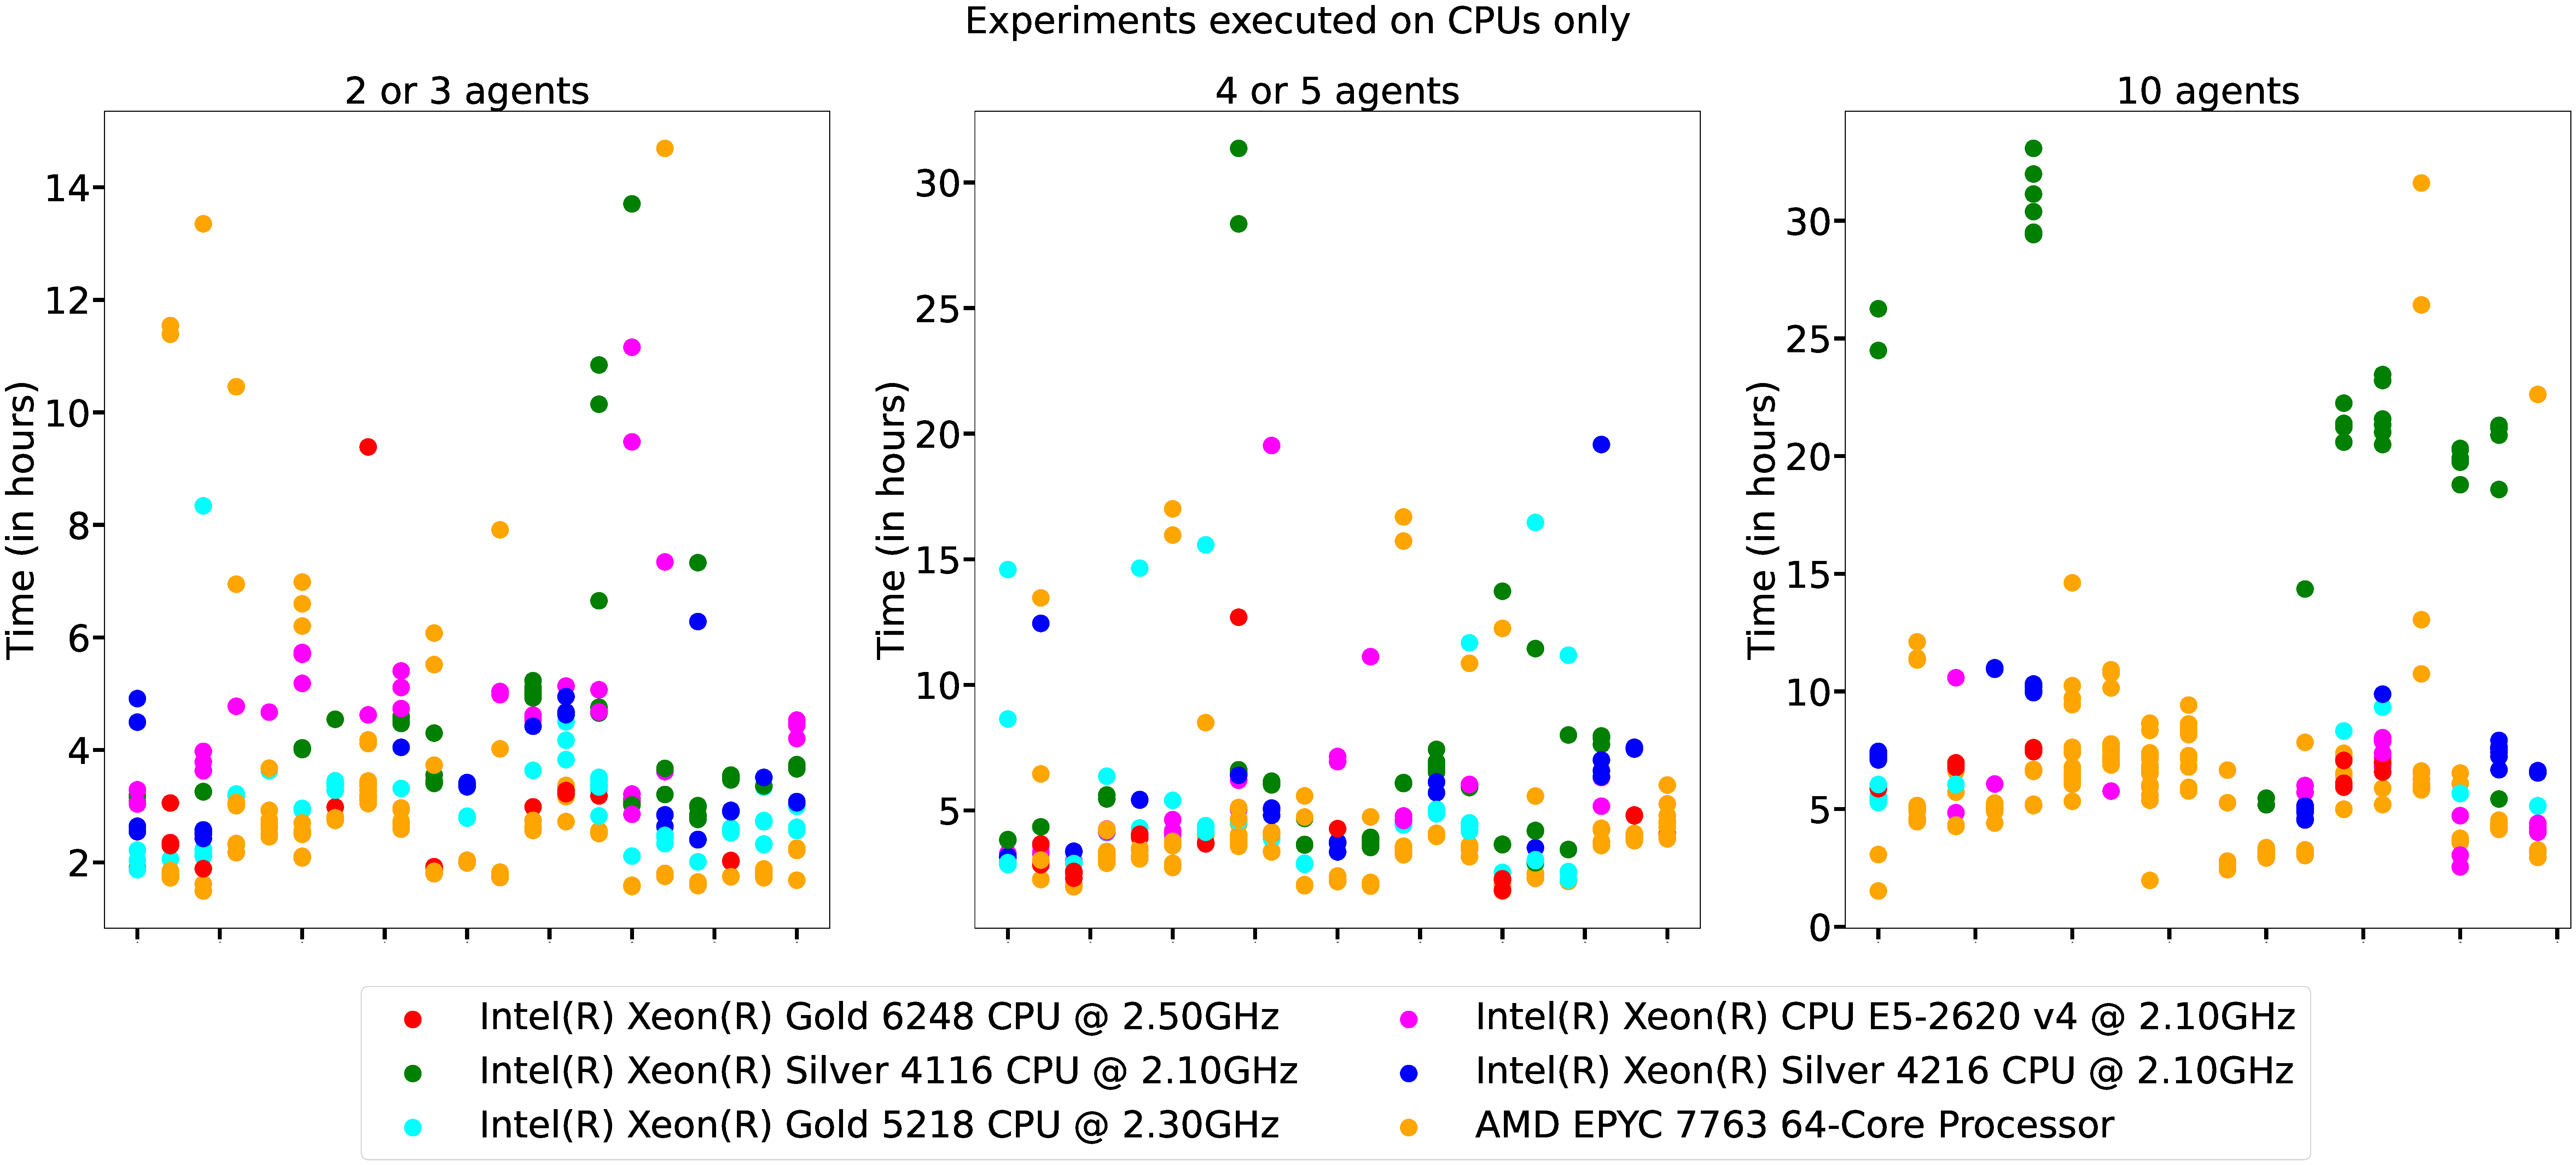
\includegraphics[width=\textwidth]{tex_thesis/figures/ch5/training_time_cpu.pdf}
    \caption{Training duration for experiments with $n<=10$ performed on only CPUs.}
    \label{fig:training_time_cpu}
\end{figure}

\begin{figure}
    \centering
    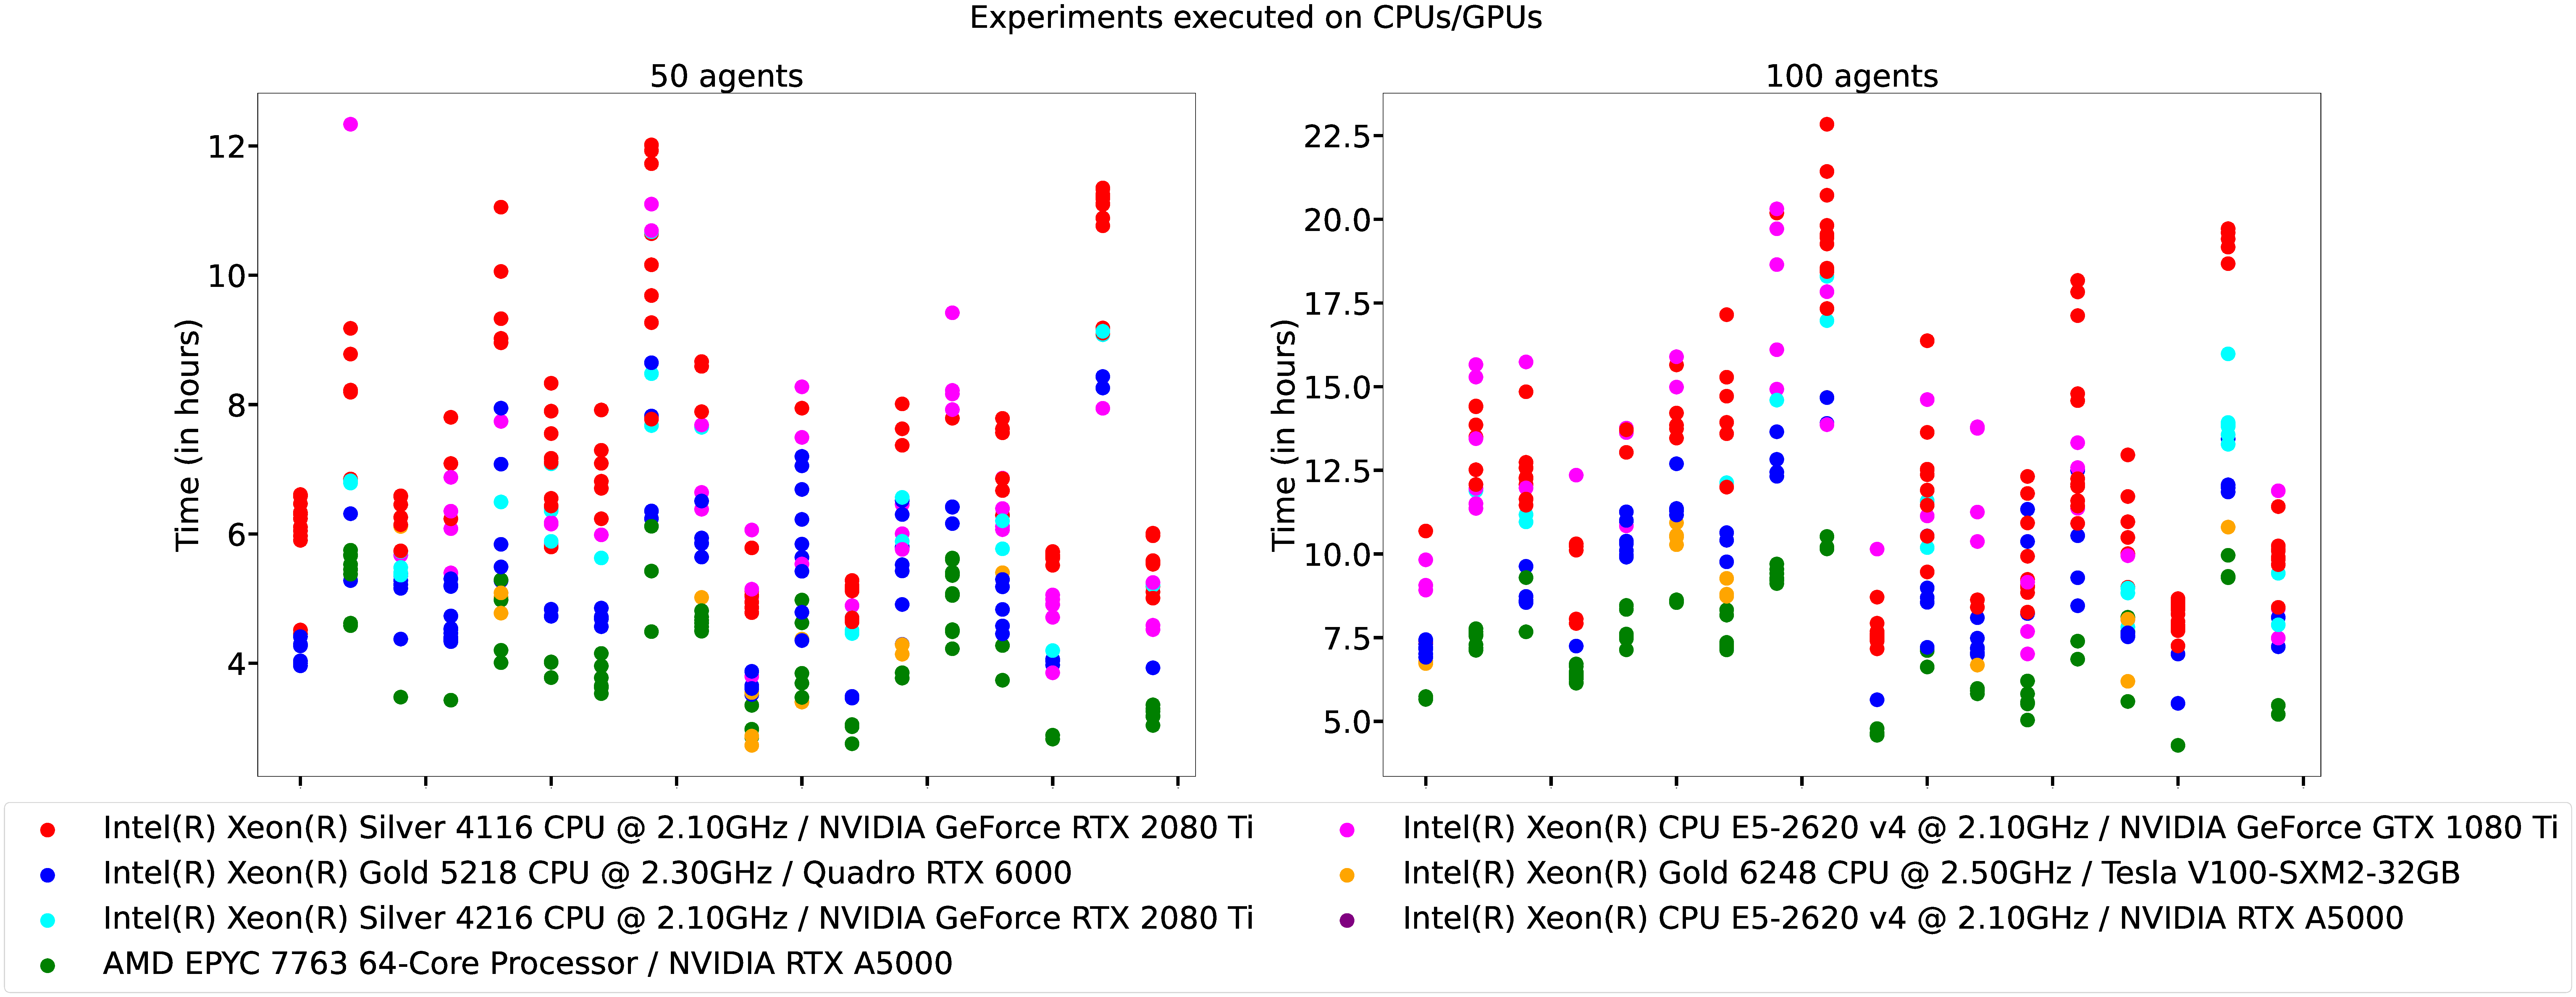
\includegraphics[width=\textwidth]{tex_thesis/figures/ch5/training_time_gpu.pdf}
    \caption{Training duration for experiments with $n>=50$ performed on CPUs and GPUs.}
    \label{fig:training_time_gpu}
\end{figure}

\begin{figure}
    \centering
    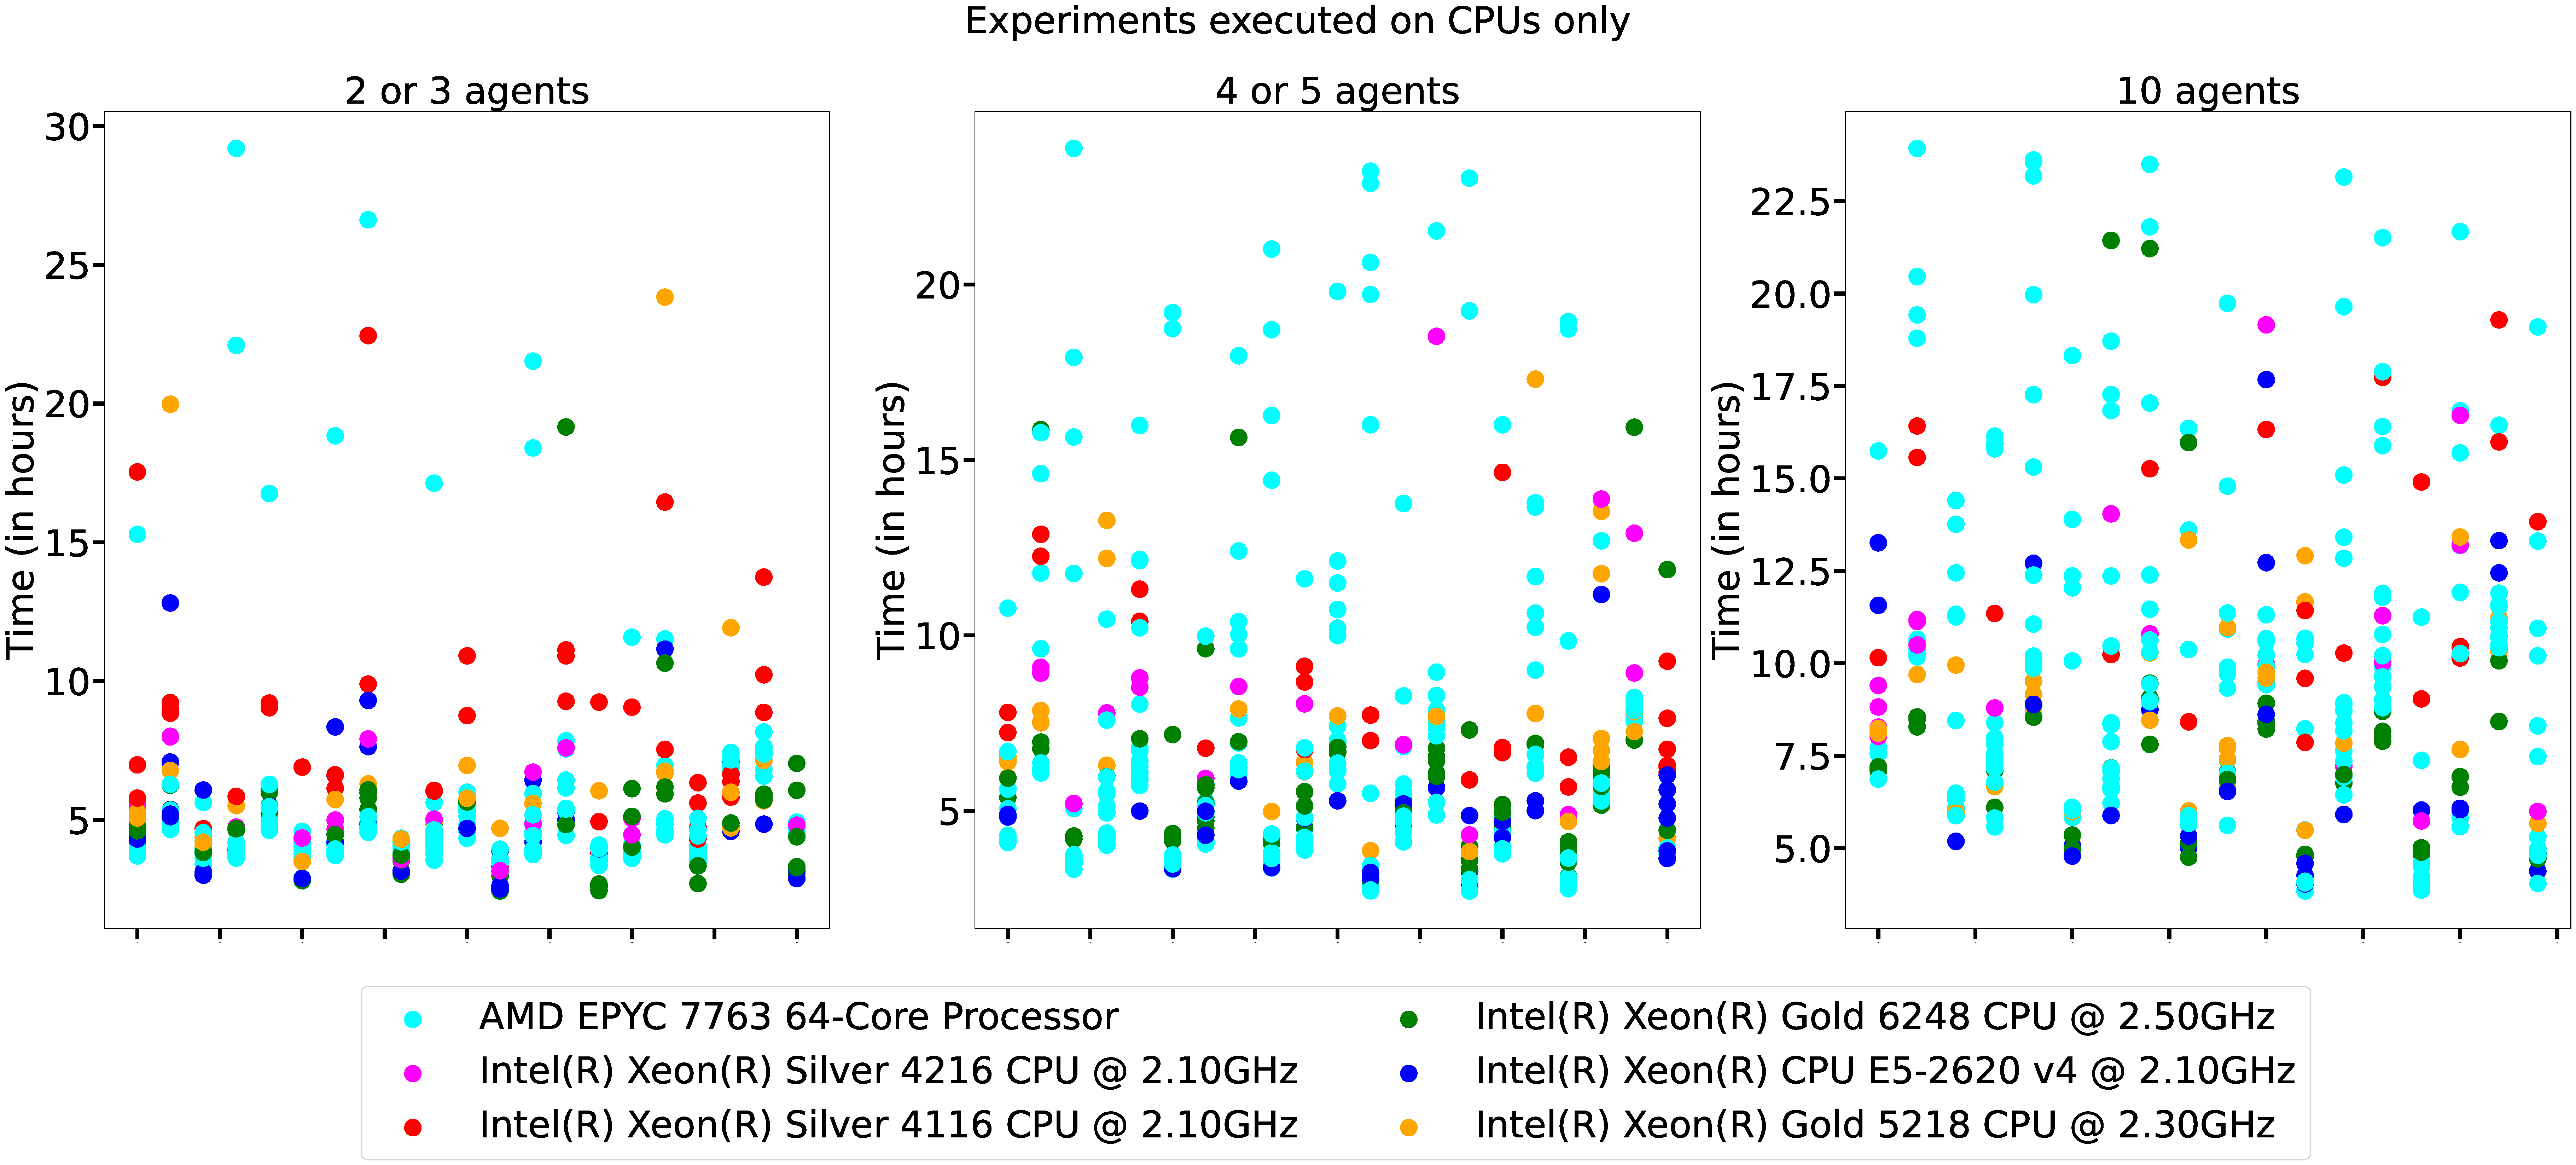
\includegraphics[width=\textwidth]{tex_thesis/figures/ch5/testing_time_cpu.pdf}
    \caption{Testing duration for experiments with $n<=10$ performed on only CPUs.}
    \label{fig:testing_time_cpu}
\end{figure}

\begin{figure}
    \centering
    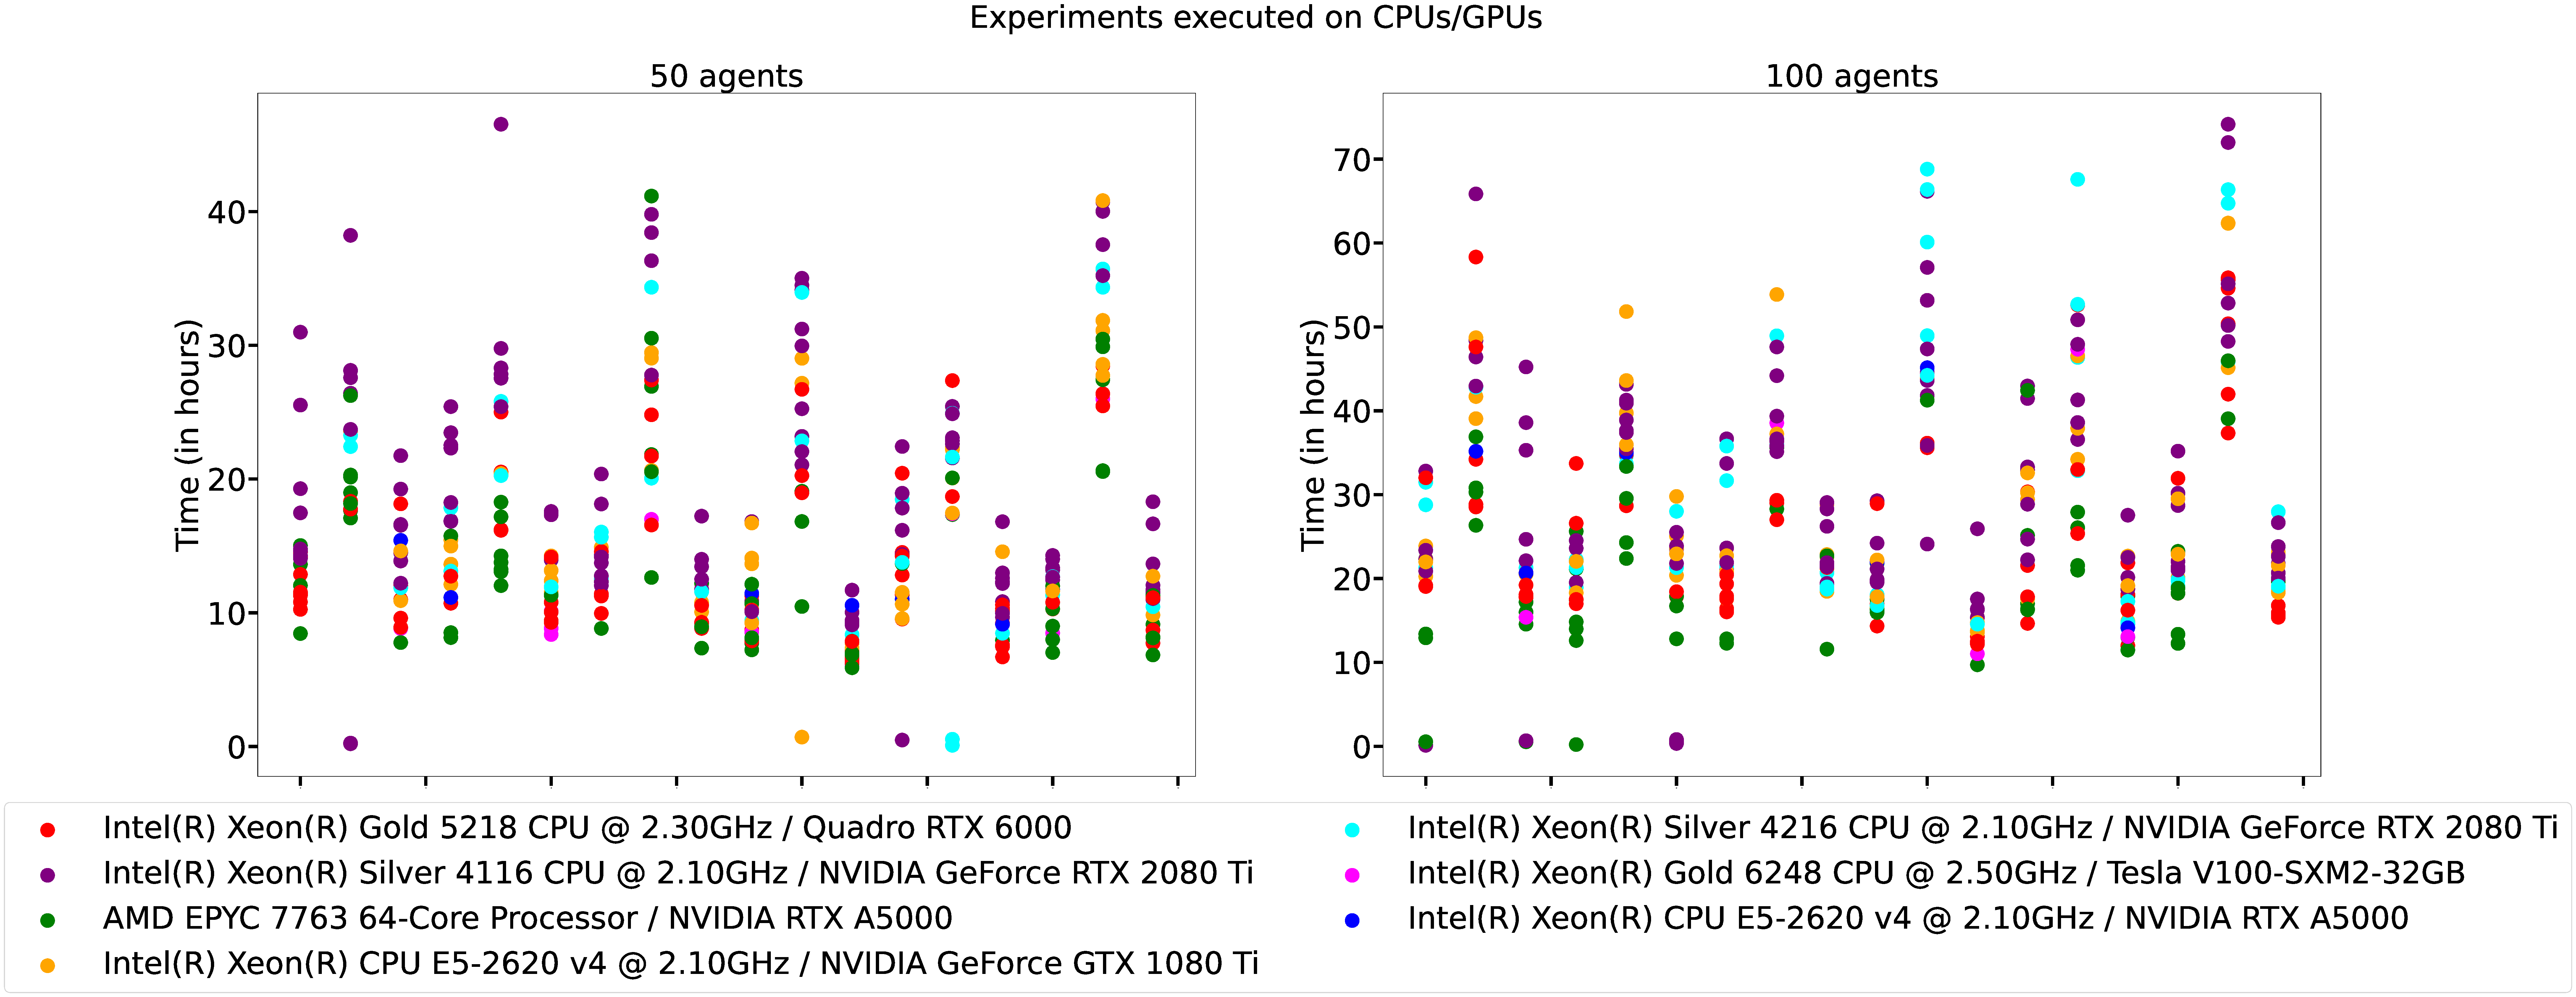
\includegraphics[width=\textwidth]{tex_thesis/figures/ch5/testing_time_gpu.pdf}
    \caption{Testing duration for experiments with $n>=50$ performed on CPUs and GPUs.}
    \label{fig:testing_time_gpu}
\end{figure}

The first observation that may be addressed is the resulting high variance. 
The variation across runs is logical because of the specific performance of the CPU/GPU models employed, but also due to the additional activity of clusters at the time of our experiments.
With respect to the computational time required for training, testing episodes are not executed and we can see that, by running the experiments on only CPUs, we manage to train the agents in less than $10$ hours, except for some occasional outliers.
For experiments with $50$ agents, and also relying on GPUs, the computational time is overall very similar to those previously mentioned, requiring less than $10$ hours, yet a longer time is needed for those with $100$ agents.
The fastest training results correspond to COMA because we are running four environments in parallel, instead of one during training.
We can see that IQL and QMIX follow closely, but QVMix, QPLEX, and FACMAC require additional computational time due to their architecture complexity.
Naturally, the testing stage needs more time compared to training for all experiments because it executes $10,000$ test episodes per stored network.
The correlated k-out-of-n environment slightly requires more time than the others because the correlation information is updated at every inspection step.


\begin{figure}
    \centering
    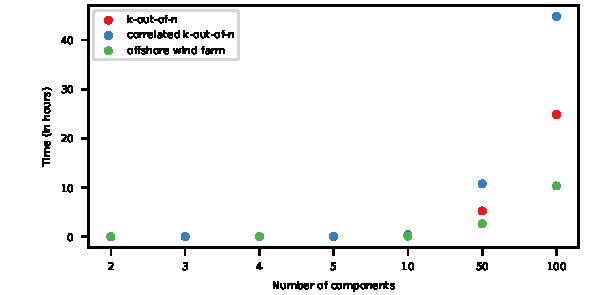
\includegraphics{tex_thesis/figures/ch5/heur_cpu_time.pdf}
    \caption{Computational time required for executing expert-based heuristic policies as a function of the number of components. The experiments are run on 2 AMD EPYC Rome 7542 CPUs @ 2.9GHz.}
    \label{fig:heur_time_cpu}
\end{figure}
Furthermore, we represent in Figure \ref{fig:heur_time_cpu} the time required for the computation of expert-based heuristic policies. The experiments are plotted as a function of the number of components and coloured based on their corresponding environment. In this case, all experiments are run on CPUs. We can see that heuristic policies can be efficiently computed for environments with less than 50 components, yet the computational time significantly increases for experiments with 50 or 100 components. This result is logical since the combination of evaluated parameters includes the number of components to be inspected at each inspection interval. Besides, the overall computation time is directly influenced by the time needed to run an episode, with the k-out-of-n environments taking longer compared to the offshore wind farm ones because the episode's finite horizon spans over 10 additional time steps. 

\subsection{Statistical analysis of the variance associated with the number of test episodes}
\label{app:variance_env}

\begin{figure}
\centering
    
\includegraphics[width=\textwidth]{tex_thesis/figures/ch5/variance_analysis.pdf}
\caption{
Variance analysis of a given set of neural networks.
We report the standard deviation of the sum of discounted rewards obtained during the test phase.
Each curve represents an entire test experiment when executing 100, 1,000, or 10,000 test episodes.
}
\label{fig:variance_details}
\end{figure}

As previously explained, we conduct 10,000 test episodes to reduce the variance related to the expected sum of discounted rewards within a given environment.
The choice is motivated by the direct relationship between the variance associated with $\mathbb{E}[R_{0}]$ and the number of test episodes. 
In our experiments, we average over 10,000 policy realisations, but here, we show that the standard deviation associated with $\mathbb{E}[R_{0}]$ for each trainig time step can vary significantly if an insufficient number of test episodes is simulated.
Figure \ref{fig:variance_details} illustrates the standard deviations observed when executing with 100, 1,000, and 10,000 test episodes.
To produce this figure, we take the neural networks obtained with one FACMAC training run.
These networks are trained over time in the offshore wind farm environment with 100 components.
From this single set of networks, we execute 10 times the 100, 1,000, and 10,000 test episodes to observe how the variance evolves with this number of test episodes.
We observe that the standard deviations of $\mathbb{E}[R_{0}]$ obtained with 100 test episodes significantly vary over the investigated test runs.
Naturally, the variation of the standard deviation is reduced with an increasing number of test episodes, obtaining very similar standard deviations when testing with 10,000 episodes.

Moreover, one can also compute the largest difference that is observed between these 10 test runs at a specific time step i.e., the absolute difference of the estimated $\mathbb{E}[R_{0}]$ at a given time step.
When testing 100 episodes, the absolute difference is $231.89$ at a time step where the maximum of the 10 provided $\mathbb{E}[R_{0}]$ is $ -2786.1$.
If 1000 episodes are tested, the absolute difference is $99.8$ where the maximum is $-2757.2$ at this time step, whereas by testing 10,000 episodes, the difference equals $24.8$ with a maximum of $-2622.8$.
These numbers represent only a trained set of networks over $1920$ training runs, and thus a final conclusion cannot be claimed, yet it motivates the need of simulating 10,000 test episodes, as with only 100 test episodes, the absolute difference can reach up to 10 \%.
\cleardoublepage
\chapter{Two-team Markov game supplementary materials} \label{ch:ch7_appendix}
\section{Training parameters}
\label{app:train_param}
The learning parameters of the three methods were determined by default configurations provided by their different authors.
They are the same as the ones used in QVMix implementation \citep{leroy2020qvmix}.
We hereafter provide a description of some of these training parameters.

Individual networks are 64 cells GRU enclosed with fully connected layers (see Fig \ref{fig:indivQ}).
The mixer network is the same as in \citep{Rashid2018} with an embedded size of 32.
The individual and mixer networks are the same for the three methods.
We used the default parameters of MAVEN policy networks provided by \citep{Mahajan2019MAVEN:Exploration}.
For QVMix, the $V$ network is a copy of the QMIX network with only one output for each $V$ network.

For each learning scenario, networks are updated regardless of how episodes have been generated.
Networks are updated from a replay buffer that collects the $5000$ latest played episodes and $32$ of them are sampled from it to update the network.
The network update is performed every eight episodes in the $3m$ map and every episode in the $3s5z$ map.
The difference is justified by the desire to increase the number of network updates for $3s5$ to improve performances, especially against the heuristic.
The epsilon greedy exploration starts with an epsilon equal to $1$ decreasing linearly to $0.05$ during $2$ million timesteps.
This is perhaps the main difference between the provided parameters, which decrease the epsilon only during $0.5$ million timesteps.
The discount factor is $\gamma = 0.99$ and the learning rate is $0.0005$.
Target networks are updated every $200$ episode.
We refer the reader to \citep{Mahajan2019MAVEN:Exploration} for further parameter definitions for MAVEN optimisation.

\section{Training time}
\label{app:train_time}

\begin{figure}[ht]
    \centering
    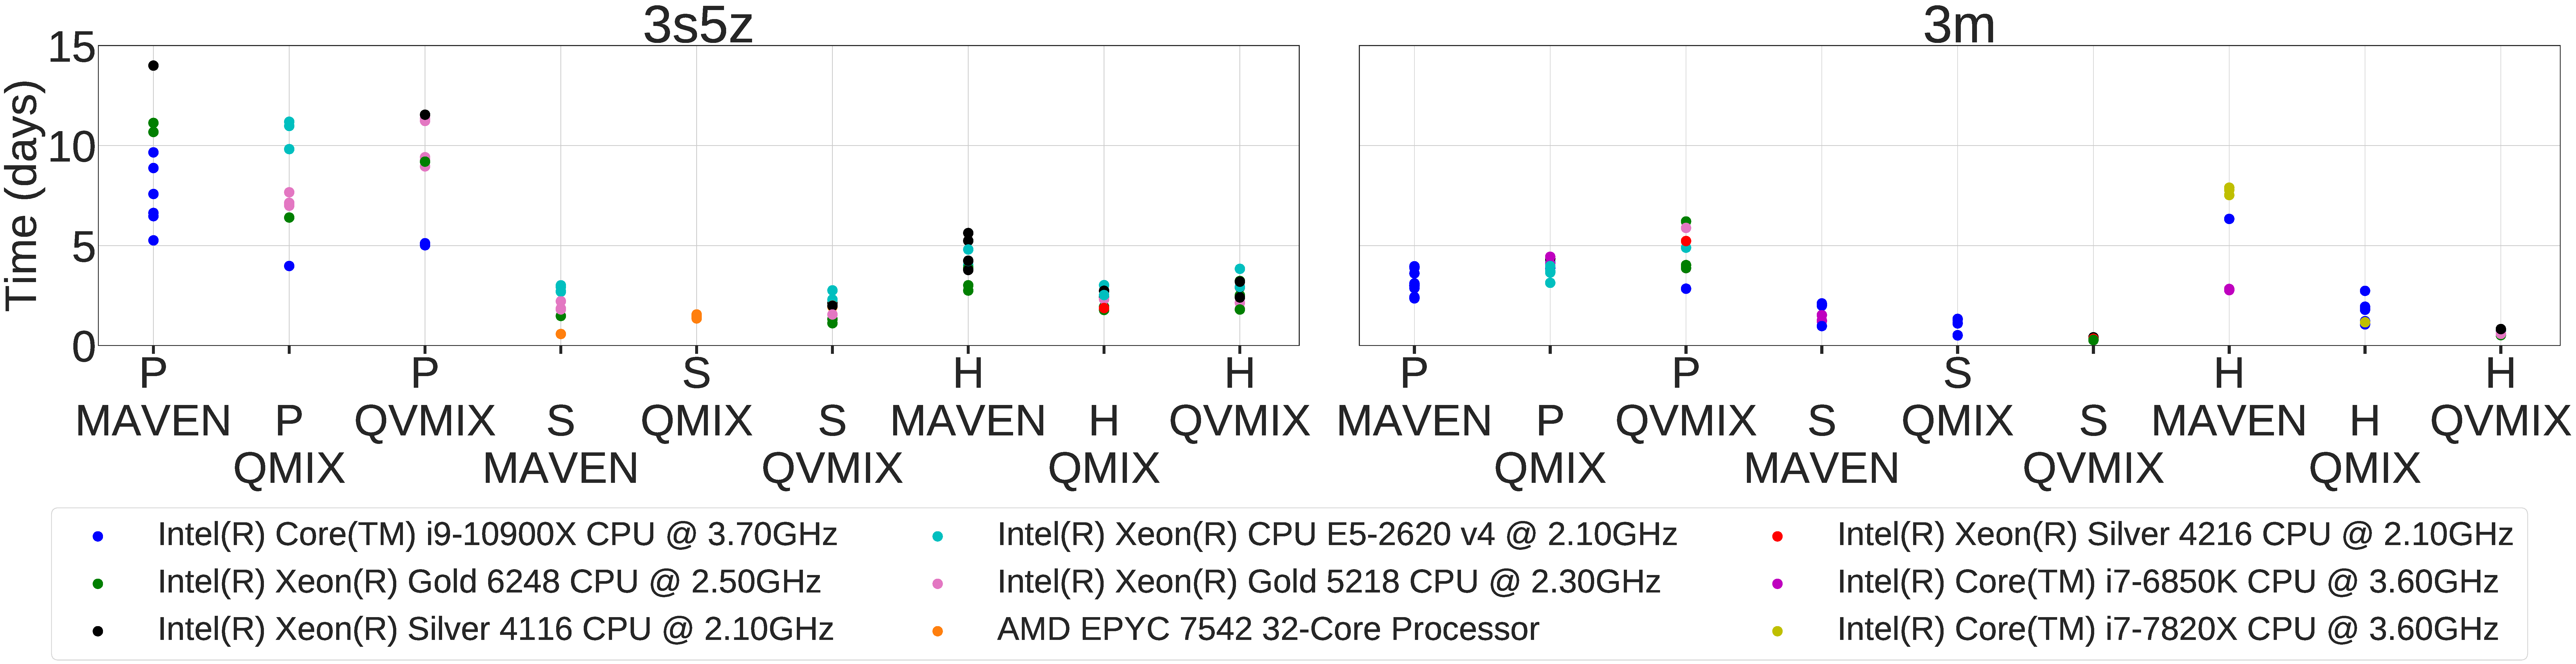
\includegraphics[width=\textwidth]{tex_thesis/figures/ch7/training_time.pdf}
    \caption{Training duration, in days, for the different learning scenarios tested in this paper.
    The different colours represent the different CPUs that have been used to perform the experiments.}
    \label{fig:training_time}
\end{figure}

Experiments were performed with CPUs only because small recurrent neural networks do not arguably benefit from GPU.
We had access to several types of computers, with different numbers of CPUs accessible at the same time.
Training times for each experiment performed are presented in Figure \ref{fig:training_time}.
With all these different hardware configurations, it is not possible to rigorously compare the times of the experiments.
However, it is possible to present the time complexity.
As explained in Section \ref{sec:experiments}, training in self-play requires five times fewer environment timesteps than training within a population but also five times fewer network updates.
Furthermore, when training a population, networks are updated sequentially, which also increases the time.
Finally, SC2 processes are prone to errors and, therefore, sometimes need to be restarted.
As the actions of all agents in the different running environments are performed simultaneously, these restarts are time-consuming operations as the processes have to wait for the faulty one.
\cleardoublepage
% \cleardoublepage% Notations ====================================================================

\chapter{Notations}

\begin{tabularx}{\textwidth}{ l X }

\end{tabularx}

\cleardoublepage% Bibliography ================================================================

\chapter{References}

\begingroup
    \def\chapter*#1{}
    \bibliographystyle{abbrvnat}
    \renewcommand{\bibname}{}
    \label{app:bibliography}
    \bibliography{bibliography}
\endgroup



\end{document}
